\documentclass[twoside]{book}

% Packages required by doxygen
\usepackage{calc}
\usepackage{doxygen}
\usepackage{graphicx}
\usepackage[utf8]{inputenc}
\usepackage{makeidx}
\usepackage{multicol}
\usepackage{multirow}
\usepackage{textcomp}
\usepackage[table]{xcolor}

% NLS support packages
\usepackage{polski}
\usepackage[T1]{fontenc}

% Font selection
\usepackage[T1]{fontenc}
\usepackage{mathptmx}
\usepackage[scaled=.90]{helvet}
\usepackage{courier}
\usepackage{amssymb}
\usepackage{sectsty}
\renewcommand{\familydefault}{\sfdefault}
\allsectionsfont{%
  \fontseries{bc}\selectfont%
  \color{darkgray}%
}
\renewcommand{\DoxyLabelFont}{%
  \fontseries{bc}\selectfont%
  \color{darkgray}%
}

% Page & text layout
\usepackage{geometry}
\geometry{%
  a4paper,%
  top=2.5cm,%
  bottom=2.5cm,%
  left=2.5cm,%
  right=2.5cm%
}
\tolerance=750
\hfuzz=15pt
\hbadness=750
\setlength{\emergencystretch}{15pt}
\setlength{\parindent}{0cm}
\setlength{\parskip}{0.2cm}
\makeatletter
\renewcommand{\paragraph}{%
  \@startsection{paragraph}{4}{0ex}{-1.0ex}{1.0ex}{%
    \normalfont\normalsize\bfseries\SS@parafont%
  }%
}
\renewcommand{\subparagraph}{%
  \@startsection{subparagraph}{5}{0ex}{-1.0ex}{1.0ex}{%
    \normalfont\normalsize\bfseries\SS@subparafont%
  }%
}
\makeatother

% Headers & footers
\usepackage{fancyhdr}
\pagestyle{fancyplain}
\fancyhead[LE]{\fancyplain{}{\bfseries\thepage}}
\fancyhead[CE]{\fancyplain{}{}}
\fancyhead[RE]{\fancyplain{}{\bfseries\leftmark}}
\fancyhead[LO]{\fancyplain{}{\bfseries\rightmark}}
\fancyhead[CO]{\fancyplain{}{}}
\fancyhead[RO]{\fancyplain{}{\bfseries\thepage}}
\fancyfoot[LE]{\fancyplain{}{}}
\fancyfoot[CE]{\fancyplain{}{}}
\fancyfoot[RE]{\fancyplain{}{\bfseries\scriptsize Wygenerowano Śr, 22 kwi 2015 23\-:00\-:56 dla lab6 programem Doxygen }}
\fancyfoot[LO]{\fancyplain{}{\bfseries\scriptsize Wygenerowano Śr, 22 kwi 2015 23\-:00\-:56 dla lab6 programem Doxygen }}
\fancyfoot[CO]{\fancyplain{}{}}
\fancyfoot[RO]{\fancyplain{}{}}
\renewcommand{\footrulewidth}{0.4pt}
\renewcommand{\chaptermark}[1]{%
  \markboth{#1}{}%
}
\renewcommand{\sectionmark}[1]{%
  \markright{\thesection\ #1}%
}

% Indices & bibliography
\usepackage{natbib}
\usepackage[titles]{tocloft}
\setcounter{tocdepth}{3}
\setcounter{secnumdepth}{5}
\makeindex

% Hyperlinks (required, but should be loaded last)
\usepackage{ifpdf}
\ifpdf
  \usepackage[pdftex,pagebackref=true]{hyperref}
\else
  \usepackage[ps2pdf,pagebackref=true]{hyperref}
\fi
\hypersetup{%
  colorlinks=true,%
  linkcolor=blue,%
  citecolor=blue,%
  unicode%
}

% Custom commands
\newcommand{\clearemptydoublepage}{%
  \newpage{\pagestyle{empty}\cleardoublepage}%
}


%===== C O N T E N T S =====

\begin{document}

% Titlepage & ToC
\hypersetup{pageanchor=false}
\pagenumbering{roman}
\begin{titlepage}
\vspace*{7cm}
\begin{center}%
{\Large lab6 \\[1ex]\large 0.\-0006 }\\
\vspace*{1cm}
{\large Wygenerowano przez Doxygen 1.8.6}\\
\vspace*{0.5cm}
{\small Śr, 22 kwi 2015 23:00:56}\\
\end{center}
\end{titlepage}
\clearemptydoublepage
\tableofcontents
\clearemptydoublepage
\pagenumbering{arabic}
\hypersetup{pageanchor=true}

%--- Begin generated contents ---
\chapter{Laboratorium 6}
\label{index}\hypertarget{index}{}\begin{DoxyAuthor}{Autor}
Filip Malinowski 
\end{DoxyAuthor}
\begin{DoxyDate}{Data}
22.\-04.\-2015 
\end{DoxyDate}
\begin{DoxyVersion}{Wersja}
0.\-0005
\end{DoxyVersion}
Program sluzacy do uruchamiania algorytmow i badania ich szybkosci dzialania.\par
W programie zaimplementowane sa algorytmy\-:\par

\begin{DoxyItemize}
\item sortowania szybkiego stosu\par

\item sortowania szybkiego po optymalizacji pivot stosu\par

\item sortowania przez scalanie stosu\par

\item sortowania przez kopcowanie stosu
\end{DoxyItemize}

Do wykonania podanych powyzej trzech ostatnich algorytmow zostaly zaimplementowane potrzebne struktury danych (stos, kolejka, lista oraz lista tablicowa, lista asocjacyjna, tablica z haszowaniem).\par
\par
Ciala klas znajduja sie w folderze ./prj/inc\par
Definicje metod znajduja sie w folderze ./prj/src\par
Sprawozdanie znajduje sie w folderze ./prj/doc/sprawozdanie\par
\par
Format wywolania\-:\par

\begin{DoxyCode}
./prj/make clean\(\backslash\)n
./prj/make\(\backslash\)n
\end{DoxyCode}
 
\chapter{Indeks hierarchiczny}
\section{Hierarchia klas}
Ta lista dziedziczenia posortowana jest z grubsza, choć nie całkowicie, alfabetycznie\-:\begin{DoxyCompactList}
\item \contentsline{section}{Benchmark}{\pageref{class_benchmark}}{}
\begin{DoxyCompactList}
\item \contentsline{section}{Mnozenie}{\pageref{class_mnozenie}}{}
\end{DoxyCompactList}
\end{DoxyCompactList}

\chapter{Indeks klas}
\section{Lista klas}
Tutaj znajdują się klasy, struktury, unie i interfejsy wraz z ich krótkimi opisami\-:\begin{DoxyCompactList}
\item\contentsline{section}{\hyperlink{class_algorithm_kolejka}{Algorithm\-Kolejka} \\*Klasa \hyperlink{class_algorithm_kolejka}{Algorithm\-Kolejka} modelujaca algorytm wczytywania do kolejki. Obiekt tego typu reprezentuje algorytm wykonujacy wykonujacy wczytywanie zadanej ilosci elementow do kolejki }{\pageref{class_algorithm_kolejka}}{}
\item\contentsline{section}{\hyperlink{class_algorithm_lista}{Algorithm\-Lista} \\*Klasa \hyperlink{class_algorithm_lista}{Algorithm\-Lista} modelujaca algorytm wczytywania do kolejki. Obiekt tego typu reprezentuje algorytm wykonujacy wykonujacy wczytywanie zadanej ilosci elementow do listy }{\pageref{class_algorithm_lista}}{}
\item\contentsline{section}{\hyperlink{class_algorithm_stos}{Algorithm\-Stos} \\*Klasa \hyperlink{class_algorithm_stos}{Algorithm\-Stos} modelujaca algorytm wczytywania do stosu. Obiekt tego typu reprezentuje algorytm wykonujacy wykonujacy wczytywanie zadanej ilosci elementow do stosu }{\pageref{class_algorithm_stos}}{}
\item\contentsline{section}{\hyperlink{class_benchmark}{Benchmark} \\*Klasa \hyperlink{class_benchmark}{Benchmark} modelujaca program benchmarkujacy. Obiekt tego typu reprezentuje program sprawdzajacy szybkosc wykonywania algorytmow }{\pageref{class_benchmark}}{}
\item\contentsline{section}{\hyperlink{class_kolejka}{Kolejka} \\*Klasa \hyperlink{class_kolejka}{Kolejka} modelujaca strukture danych typu kolejka. Obiekt tego typu reprezentuje strukture danych typu kolejka wraz z operacjami mozliwymi do wykonania na tej strukturze }{\pageref{class_kolejka}}{}
\item\contentsline{section}{\hyperlink{struct_lista_1_1_komorka}{Lista\-::\-Komorka} \\*Struktura \hyperlink{struct_lista_1_1_komorka}{Komorka}. Obiekt tego typu reprezentuje pojedyncza komorke wraz ze wskaznikiem na nastepna komorke listy }{\pageref{struct_lista_1_1_komorka}}{}
\item\contentsline{section}{\hyperlink{class_lista}{Lista} \\*Klasa \hyperlink{class_lista}{Lista} modelujaca strukture danych typu lista. Obiekt tego typu reprezentuje strukture danych typu lista wraz z operacjami mozliwymi do wykonania na tej strukturze }{\pageref{class_lista}}{}
\item\contentsline{section}{\hyperlink{class_mnozenie}{Mnozenie} \\*Klasa \hyperlink{class_mnozenie}{Mnozenie} modelujaca algorytm mnozenia. Obiekt tego typu reprezentuje algorytm wykonujacy dzialanie mnozenia kazdego elementu tablicy tab przez 2 }{\pageref{class_mnozenie}}{}
\item\contentsline{section}{\hyperlink{class_stos}{Stos} \\*Klasa \hyperlink{class_stos}{Stos} modelujaca strukture danych typu stos. Obiekt tego typu reprezentuje strukture danych typu stos wraz z operacjami mozliwymi do wykonania na tej strukturze }{\pageref{class_stos}}{}
\end{DoxyCompactList}

\chapter{Indeks plików}
\section{Lista plików}
Tutaj znajduje się lista wszystkich plików z ich krótkimi opisami\-:\begin{DoxyCompactList}
\item\contentsline{section}{\hyperlink{algorithm2_8cpp}{algorithm2.\-cpp} }{\pageref{algorithm2_8cpp}}{}
\item\contentsline{section}{\hyperlink{algorithm2_8hh}{algorithm2.\-hh} }{\pageref{algorithm2_8hh}}{}
\item\contentsline{section}{\hyperlink{algorithm__kolejka_8cpp}{algorithm\-\_\-kolejka.\-cpp} }{\pageref{algorithm__kolejka_8cpp}}{}
\item\contentsline{section}{\hyperlink{algorithm__kolejka_8hh}{algorithm\-\_\-kolejka.\-hh} }{\pageref{algorithm__kolejka_8hh}}{}
\item\contentsline{section}{\hyperlink{algorithm__lista_8cpp}{algorithm\-\_\-lista.\-cpp} }{\pageref{algorithm__lista_8cpp}}{}
\item\contentsline{section}{\hyperlink{algorithm__lista_8hh}{algorithm\-\_\-lista.\-hh} }{\pageref{algorithm__lista_8hh}}{}
\item\contentsline{section}{\hyperlink{algorithm__stos_8cpp}{algorithm\-\_\-stos.\-cpp} }{\pageref{algorithm__stos_8cpp}}{}
\item\contentsline{section}{\hyperlink{algorithm__stos_8hh}{algorithm\-\_\-stos.\-hh} }{\pageref{algorithm__stos_8hh}}{}
\item\contentsline{section}{\hyperlink{benchmark_8cpp}{benchmark.\-cpp} }{\pageref{benchmark_8cpp}}{}
\item\contentsline{section}{\hyperlink{benchmark_8hh}{benchmark.\-hh} }{\pageref{benchmark_8hh}}{}
\item\contentsline{section}{\hyperlink{generate_8cpp}{generate.\-cpp} }{\pageref{generate_8cpp}}{}
\item\contentsline{section}{\hyperlink{kolejka_8cpp}{kolejka.\-cpp} }{\pageref{kolejka_8cpp}}{}
\item\contentsline{section}{\hyperlink{kolejka_8hh}{kolejka.\-hh} }{\pageref{kolejka_8hh}}{}
\item\contentsline{section}{\hyperlink{lista_8cpp}{lista.\-cpp} }{\pageref{lista_8cpp}}{}
\item\contentsline{section}{\hyperlink{lista_8hh}{lista.\-hh} }{\pageref{lista_8hh}}{}
\item\contentsline{section}{\hyperlink{main_8cpp}{main.\-cpp} }{\pageref{main_8cpp}}{}
\item\contentsline{section}{\hyperlink{stos_8cpp}{stos.\-cpp} }{\pageref{stos_8cpp}}{}
\item\contentsline{section}{\hyperlink{stos_8hh}{stos.\-hh} }{\pageref{stos_8hh}}{}
\item\contentsline{section}{\hyperlink{tab__lista_8cpp}{tab\-\_\-lista.\-cpp} }{\pageref{tab__lista_8cpp}}{}
\item\contentsline{section}{\hyperlink{tab__lista_8hh}{tab\-\_\-lista.\-hh} }{\pageref{tab__lista_8hh}}{}
\end{DoxyCompactList}

\chapter{Dokumentacja klas}
\hypertarget{class_algorithm1}{\section{Dokumentacja klasy Algorithm1}
\label{class_algorithm1}\index{Algorithm1@{Algorithm1}}
}


Klasa \hyperlink{class_algorithm1}{Algorithm1} modelujaca algorytm sortowania stosu. Obiekt tego typu reprezentuje algorytm wykonujacy sortowanie szybkie na elementach stosu.  




{\ttfamily \#include $<$algorithm1.\-hh$>$}



Diagram dziedziczenia dla Algorithm1\nopagebreak
\begin{figure}[H]
\begin{center}
\leavevmode
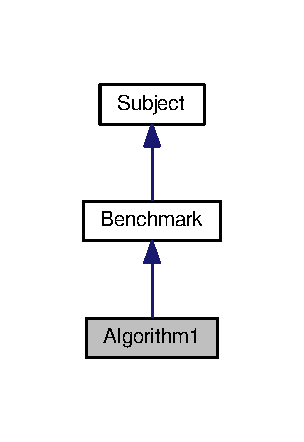
\includegraphics[width=146pt]{class_algorithm1__inherit__graph}
\end{center}
\end{figure}


Diagram współpracy dla Algorithm1\-:\nopagebreak
\begin{figure}[H]
\begin{center}
\leavevmode
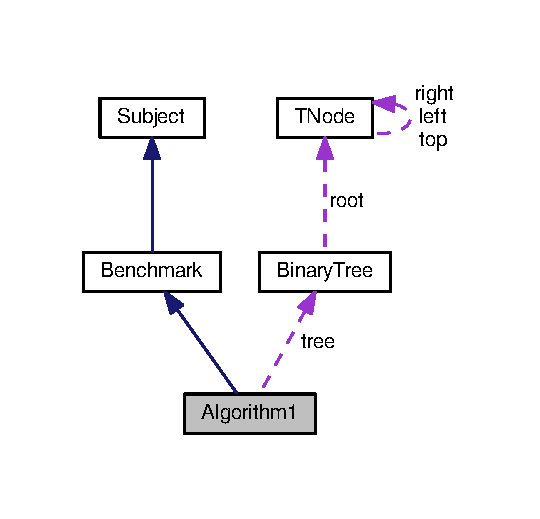
\includegraphics[width=201pt]{class_algorithm1__coll__graph}
\end{center}
\end{figure}
\subsection*{Metody publiczne}
\begin{DoxyCompactItemize}
\item 
\hyperlink{class_algorithm1_ad2b1593378788a36b954b65d1c2af8ff}{Algorithm1} ()
\begin{DoxyCompactList}\small\item\em Konstruktor obiektu \hyperlink{class_algorithm1}{Algorithm1}. \end{DoxyCompactList}\item 
\hyperlink{class_algorithm1_ad2976b6058bd8886cfd20307e79b6042}{Algorithm1} (int $\ast$\-\_\-tab)
\begin{DoxyCompactList}\small\item\em Konstruktor parametryczny obiektu \hyperlink{class_algorithm1}{Algorithm1}. \end{DoxyCompactList}\item 
\hyperlink{class_algorithm1_afbd4d69811879472fcadb25a1c3c5262}{$\sim$\-Algorithm1} ()
\begin{DoxyCompactList}\small\item\em Destruktor obiektu \hyperlink{class_algorithm1}{Algorithm1}. \end{DoxyCompactList}\item 
virtual void \hyperlink{class_algorithm1_a35260610f8093c3812a6f146147955e6}{test\-Algorithm} (\hyperlink{class_benchmark}{Benchmark} $\ast$\-\_\-algorithm)
\begin{DoxyCompactList}\small\item\em Metoda testowania algorytmu. Metoda sluzy do testowania szybkosci dzialania algorytmu. W klasie \hyperlink{class_algorithm1}{Algorithm1} nie ma konkretnego dzialania. \end{DoxyCompactList}\item 
virtual void \hyperlink{class_algorithm1_a008c8fdd07c39219099afe14e63e447a}{load} (int \-\_\-border)
\begin{DoxyCompactList}\small\item\em Metoda przygotowywania algorytmu. Metoda sluzy do przygotowania warunkow do przeprowadzenia testu. \end{DoxyCompactList}\item 
virtual void \hyperlink{class_algorithm1_a135dd26c6c741812d75cd7f2f270592d}{unload} (int \-\_\-border)
\begin{DoxyCompactList}\small\item\em Metoda sprzatania. Metoda sluzy do oproznienia struktury. \end{DoxyCompactList}\item 
virtual void \hyperlink{class_algorithm1_a671a2162843b588704044420c9a5dfa9}{run\-Algorithm} (int \-\_\-border)
\begin{DoxyCompactList}\small\item\em Metoda uruchamiania algorytmu. Metoda sluzy do wykonywania danego algorytmu. Sortuje elementy stosu. \end{DoxyCompactList}\end{DoxyCompactItemize}
\subsection*{Atrybuty prywatne}
\begin{DoxyCompactItemize}
\item 
int $\ast$ \hyperlink{class_algorithm1_a696e1e45bff4a0510dfb76274321583f}{tab}
\begin{DoxyCompactList}\small\item\em Wskaznik na tablice elementow z danymi wejsciowymi. \end{DoxyCompactList}\item 
\hyperlink{class_stos}{Stos} \hyperlink{class_algorithm1_a3fb7f66d1e4aae77a49c6f7c241f47c9}{stos}
\begin{DoxyCompactList}\small\item\em Zmienna przechowujaca stos. \end{DoxyCompactList}\end{DoxyCompactItemize}


\subsection{Opis szczegółowy}


Definicja w linii 9 pliku algorithm1.\-hh.



\subsection{Dokumentacja konstruktora i destruktora}
\hypertarget{class_algorithm1_ad2b1593378788a36b954b65d1c2af8ff}{\index{Algorithm1@{Algorithm1}!Algorithm1@{Algorithm1}}
\index{Algorithm1@{Algorithm1}!Algorithm1@{Algorithm1}}
\subsubsection[{Algorithm1}]{\setlength{\rightskip}{0pt plus 5cm}Algorithm1\-::\-Algorithm1 (
\begin{DoxyParamCaption}
{}
\end{DoxyParamCaption}
)\hspace{0.3cm}{\ttfamily [inline]}}}\label{class_algorithm1_ad2b1593378788a36b954b65d1c2af8ff}


Definicja w linii 24 pliku algorithm1.\-hh.

\hypertarget{class_algorithm1_ad2976b6058bd8886cfd20307e79b6042}{\index{Algorithm1@{Algorithm1}!Algorithm1@{Algorithm1}}
\index{Algorithm1@{Algorithm1}!Algorithm1@{Algorithm1}}
\subsubsection[{Algorithm1}]{\setlength{\rightskip}{0pt plus 5cm}Algorithm1\-::\-Algorithm1 (
\begin{DoxyParamCaption}
\item[{int $\ast$}]{\-\_\-tab}
\end{DoxyParamCaption}
)\hspace{0.3cm}{\ttfamily [inline]}}}\label{class_algorithm1_ad2976b6058bd8886cfd20307e79b6042}

\begin{DoxyParams}[1]{Parametry}
\mbox{\tt in}  & {\em \-\_\-tab} & -\/ tablica przechowujaca dane wejsciowe. \\
\hline
\end{DoxyParams}


Definicja w linii 30 pliku algorithm1.\-hh.

\hypertarget{class_algorithm1_afbd4d69811879472fcadb25a1c3c5262}{\index{Algorithm1@{Algorithm1}!$\sim$\-Algorithm1@{$\sim$\-Algorithm1}}
\index{$\sim$\-Algorithm1@{$\sim$\-Algorithm1}!Algorithm1@{Algorithm1}}
\subsubsection[{$\sim$\-Algorithm1}]{\setlength{\rightskip}{0pt plus 5cm}Algorithm1\-::$\sim$\-Algorithm1 (
\begin{DoxyParamCaption}
{}
\end{DoxyParamCaption}
)\hspace{0.3cm}{\ttfamily [inline]}}}\label{class_algorithm1_afbd4d69811879472fcadb25a1c3c5262}


Definicja w linii 35 pliku algorithm1.\-hh.



\subsection{Dokumentacja funkcji składowych}
\hypertarget{class_algorithm1_a008c8fdd07c39219099afe14e63e447a}{\index{Algorithm1@{Algorithm1}!load@{load}}
\index{load@{load}!Algorithm1@{Algorithm1}}
\subsubsection[{load}]{\setlength{\rightskip}{0pt plus 5cm}void Algorithm1\-::load (
\begin{DoxyParamCaption}
\item[{int}]{\-\_\-border}
\end{DoxyParamCaption}
)\hspace{0.3cm}{\ttfamily [virtual]}}}\label{class_algorithm1_a008c8fdd07c39219099afe14e63e447a}

\begin{DoxyParams}[1]{Parametry}
\mbox{\tt in}  & {\em \-\_\-border} & -\/ ilosc elementow dla ktorych metoda ma wykonac swoje dzialanie. \\
\hline
\end{DoxyParams}


Reimplementowana z \hyperlink{class_benchmark_a935c57201a5d0b9589a898df38b8b5a3}{Benchmark}.



Definicja w linii 15 pliku algorithm1.\-cpp.



Oto graf wywołań dla tej funkcji\-:\nopagebreak
\begin{figure}[H]
\begin{center}
\leavevmode
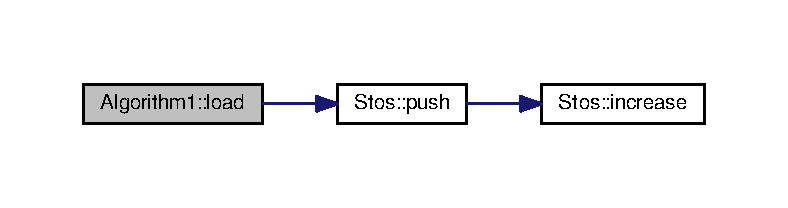
\includegraphics[width=350pt]{class_algorithm1_a008c8fdd07c39219099afe14e63e447a_cgraph}
\end{center}
\end{figure}


\hypertarget{class_algorithm1_a671a2162843b588704044420c9a5dfa9}{\index{Algorithm1@{Algorithm1}!run\-Algorithm@{run\-Algorithm}}
\index{run\-Algorithm@{run\-Algorithm}!Algorithm1@{Algorithm1}}
\subsubsection[{run\-Algorithm}]{\setlength{\rightskip}{0pt plus 5cm}void Algorithm1\-::run\-Algorithm (
\begin{DoxyParamCaption}
\item[{int}]{\-\_\-border}
\end{DoxyParamCaption}
)\hspace{0.3cm}{\ttfamily [virtual]}}}\label{class_algorithm1_a671a2162843b588704044420c9a5dfa9}

\begin{DoxyParams}[1]{Parametry}
\mbox{\tt in}  & {\em \-\_\-border} & -\/ ilosc elementow dla ktorych algorytm ma wykonac swoje dzialanie. \\
\hline
\end{DoxyParams}


Reimplementowana z \hyperlink{class_benchmark_a6363894c058e8bfe146de09d7126b29c}{Benchmark}.



Definicja w linii 9 pliku algorithm1.\-cpp.



Oto graf wywołań dla tej funkcji\-:\nopagebreak
\begin{figure}[H]
\begin{center}
\leavevmode
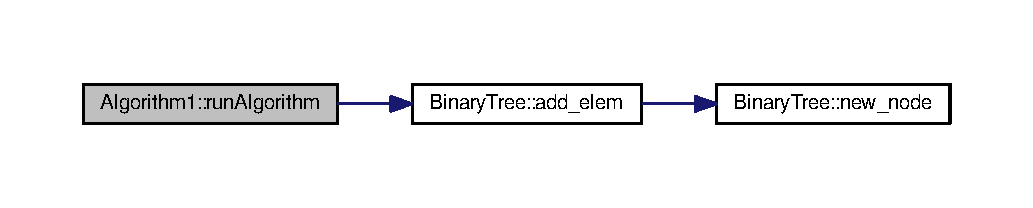
\includegraphics[width=320pt]{class_algorithm1_a671a2162843b588704044420c9a5dfa9_cgraph}
\end{center}
\end{figure}


\hypertarget{class_algorithm1_a35260610f8093c3812a6f146147955e6}{\index{Algorithm1@{Algorithm1}!test\-Algorithm@{test\-Algorithm}}
\index{test\-Algorithm@{test\-Algorithm}!Algorithm1@{Algorithm1}}
\subsubsection[{test\-Algorithm}]{\setlength{\rightskip}{0pt plus 5cm}virtual void Algorithm1\-::test\-Algorithm (
\begin{DoxyParamCaption}
\item[{{\bf Benchmark} $\ast$}]{\-\_\-algorithm}
\end{DoxyParamCaption}
)\hspace{0.3cm}{\ttfamily [inline]}, {\ttfamily [virtual]}}}\label{class_algorithm1_a35260610f8093c3812a6f146147955e6}

\begin{DoxyParams}[1]{Parametry}
\mbox{\tt in}  & {\em \-\_\-algorithm} & -\/ testowany algorytm. \\
\hline
\end{DoxyParams}


Definicja w linii 43 pliku algorithm1.\-hh.

\hypertarget{class_algorithm1_a135dd26c6c741812d75cd7f2f270592d}{\index{Algorithm1@{Algorithm1}!unload@{unload}}
\index{unload@{unload}!Algorithm1@{Algorithm1}}
\subsubsection[{unload}]{\setlength{\rightskip}{0pt plus 5cm}void Algorithm1\-::unload (
\begin{DoxyParamCaption}
\item[{int}]{\-\_\-border}
\end{DoxyParamCaption}
)\hspace{0.3cm}{\ttfamily [virtual]}}}\label{class_algorithm1_a135dd26c6c741812d75cd7f2f270592d}

\begin{DoxyParams}[1]{Parametry}
\mbox{\tt in}  & {\em \-\_\-border} & -\/ ilosc elementow dla ktorych metoda ma wykonac swoje dzialanie. \\
\hline
\end{DoxyParams}


Reimplementowana z \hyperlink{class_benchmark_aafd856205ecb699568533fff0be01209}{Benchmark}.



Definicja w linii 21 pliku algorithm1.\-cpp.



Oto graf wywołań dla tej funkcji\-:\nopagebreak
\begin{figure}[H]
\begin{center}
\leavevmode
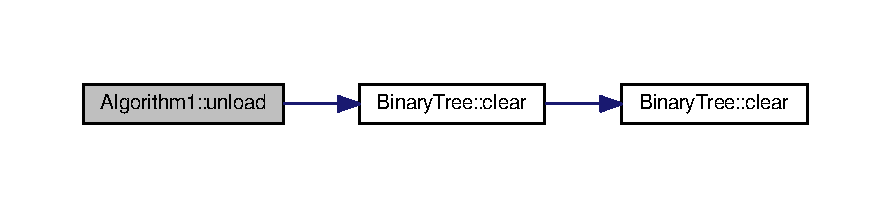
\includegraphics[width=350pt]{class_algorithm1_a135dd26c6c741812d75cd7f2f270592d_cgraph}
\end{center}
\end{figure}




\subsection{Dokumentacja atrybutów składowych}
\hypertarget{class_algorithm1_a3fb7f66d1e4aae77a49c6f7c241f47c9}{\index{Algorithm1@{Algorithm1}!stos@{stos}}
\index{stos@{stos}!Algorithm1@{Algorithm1}}
\subsubsection[{stos}]{\setlength{\rightskip}{0pt plus 5cm}{\bf Stos} Algorithm1\-::stos\hspace{0.3cm}{\ttfamily [private]}}}\label{class_algorithm1_a3fb7f66d1e4aae77a49c6f7c241f47c9}


Definicja w linii 18 pliku algorithm1.\-hh.

\hypertarget{class_algorithm1_a696e1e45bff4a0510dfb76274321583f}{\index{Algorithm1@{Algorithm1}!tab@{tab}}
\index{tab@{tab}!Algorithm1@{Algorithm1}}
\subsubsection[{tab}]{\setlength{\rightskip}{0pt plus 5cm}int$\ast$ Algorithm1\-::tab\hspace{0.3cm}{\ttfamily [private]}}}\label{class_algorithm1_a696e1e45bff4a0510dfb76274321583f}


Definicja w linii 14 pliku algorithm1.\-hh.



Dokumentacja dla tej klasy została wygenerowana z plików\-:\begin{DoxyCompactItemize}
\item 
\hyperlink{algorithm1_8hh}{algorithm1.\-hh}\item 
\hyperlink{algorithm1_8cpp}{algorithm1.\-cpp}\end{DoxyCompactItemize}

\hypertarget{class_algorithm2}{\section{Dokumentacja klasy Algorithm2}
\label{class_algorithm2}\index{Algorithm2@{Algorithm2}}
}


Klasa \hyperlink{class_algorithm2}{Algorithm2} modelujaca algorytm sortowania stosu. Obiekt tego typu reprezentuje algorytm wykonujacy sortowanie szybkie na elementach stosu. Dziedziczy po klasie \hyperlink{class_benchmark}{Benchmark}.  




{\ttfamily \#include $<$algorithm2.\-hh$>$}



Diagram dziedziczenia dla Algorithm2\nopagebreak
\begin{figure}[H]
\begin{center}
\leavevmode
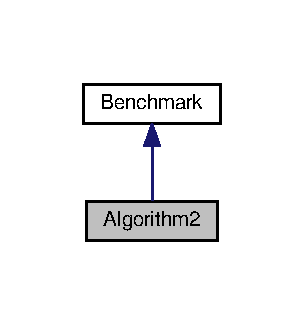
\includegraphics[width=146pt]{class_algorithm2__inherit__graph}
\end{center}
\end{figure}


Diagram współpracy dla Algorithm2\-:\nopagebreak
\begin{figure}[H]
\begin{center}
\leavevmode
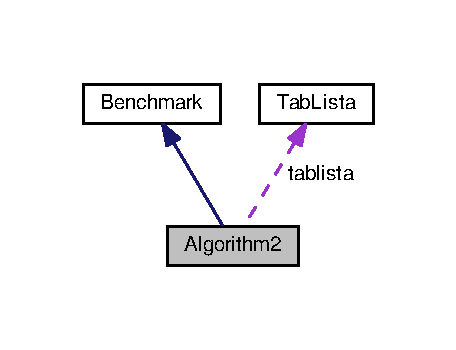
\includegraphics[width=259pt]{class_algorithm2__coll__graph}
\end{center}
\end{figure}
\subsection*{Metody publiczne}
\begin{DoxyCompactItemize}
\item 
\hyperlink{class_algorithm2_ad77a51433815456eca8139444e78b49b}{Algorithm2} ()
\begin{DoxyCompactList}\small\item\em Konstruktor obiektu \hyperlink{class_algorithm2}{Algorithm2}. \end{DoxyCompactList}\item 
\hyperlink{class_algorithm2_a63a761a11070a07905229137034b3cb9}{Algorithm2} (unsigned short $\ast$\-\_\-tab, int \-\_\-id)
\begin{DoxyCompactList}\small\item\em Konstruktor parametryczny obiektu \hyperlink{class_algorithm2}{Algorithm2}. \end{DoxyCompactList}\item 
\hyperlink{class_algorithm2_ab2c630f56f5d2e90f62a13fdaf0cd954}{$\sim$\-Algorithm2} ()
\begin{DoxyCompactList}\small\item\em Destruktor obiektu \hyperlink{class_algorithm2}{Algorithm2}. \end{DoxyCompactList}\item 
virtual void \hyperlink{class_algorithm2_a50bbb4421660c4200dba66e9da9d7969}{load} (int \-\_\-border)
\begin{DoxyCompactList}\small\item\em Metoda przygotowywania algorytmu. Metoda sluzy do przygotowania warunkow do przeprowadzenia testu. \end{DoxyCompactList}\item 
virtual void \hyperlink{class_algorithm2_a3d7e4d0c9308d0b97250cb5596a73165}{unload} (int \-\_\-border)
\begin{DoxyCompactList}\small\item\em Metoda sprzatania. Metoda sluzy do oproznienia struktury. \end{DoxyCompactList}\item 
virtual void \hyperlink{class_algorithm2_a409e58d5fb0b6d2407cc986cf163703b}{run\-Algorithm} (int \-\_\-border)
\begin{DoxyCompactList}\small\item\em Metoda uruchamiania algorytmu. Metoda sluzy do wykonywania danego algorytmu. Sortuje elementy stosu. \end{DoxyCompactList}\end{DoxyCompactItemize}
\subsection*{Atrybuty prywatne}
\begin{DoxyCompactItemize}
\item 
\hyperlink{struct_binary_tree}{Binary\-Tree} \hyperlink{class_algorithm2_aff7c12a2dc0294d120a36ae0efc4af6a}{tree}
\begin{DoxyCompactList}\small\item\em Zmienna przechowujaca drzewo binarne. \end{DoxyCompactList}\end{DoxyCompactItemize}
\subsection*{Dodatkowe Dziedziczone Składowe}


\subsection{Opis szczegółowy}


Definicja w linii 10 pliku algorithm2.\-hh.



\subsection{Dokumentacja konstruktora i destruktora}
\hypertarget{class_algorithm2_ad77a51433815456eca8139444e78b49b}{\index{Algorithm2@{Algorithm2}!Algorithm2@{Algorithm2}}
\index{Algorithm2@{Algorithm2}!Algorithm2@{Algorithm2}}
\subsubsection[{Algorithm2}]{\setlength{\rightskip}{0pt plus 5cm}Algorithm2\-::\-Algorithm2 (
\begin{DoxyParamCaption}
{}
\end{DoxyParamCaption}
)\hspace{0.3cm}{\ttfamily [inline]}}}\label{class_algorithm2_ad77a51433815456eca8139444e78b49b}


Definicja w linii 20 pliku algorithm2.\-hh.

\hypertarget{class_algorithm2_a63a761a11070a07905229137034b3cb9}{\index{Algorithm2@{Algorithm2}!Algorithm2@{Algorithm2}}
\index{Algorithm2@{Algorithm2}!Algorithm2@{Algorithm2}}
\subsubsection[{Algorithm2}]{\setlength{\rightskip}{0pt plus 5cm}Algorithm2\-::\-Algorithm2 (
\begin{DoxyParamCaption}
\item[{unsigned short $\ast$}]{\-\_\-tab, }
\item[{int}]{\-\_\-id}
\end{DoxyParamCaption}
)}}\label{class_algorithm2_a63a761a11070a07905229137034b3cb9}

\begin{DoxyParams}[1]{Parametry}
\mbox{\tt in}  & {\em \-\_\-tab} & -\/ tablica przechowujaca dane wejsciowe. \\
\hline
\mbox{\tt in}  & {\em \-\_\-id} & -\/ identyfikator algorytmu. \\
\hline
\end{DoxyParams}


Definicja w linii 10 pliku algorithm2.\-cpp.

\hypertarget{class_algorithm2_ab2c630f56f5d2e90f62a13fdaf0cd954}{\index{Algorithm2@{Algorithm2}!$\sim$\-Algorithm2@{$\sim$\-Algorithm2}}
\index{$\sim$\-Algorithm2@{$\sim$\-Algorithm2}!Algorithm2@{Algorithm2}}
\subsubsection[{$\sim$\-Algorithm2}]{\setlength{\rightskip}{0pt plus 5cm}Algorithm2\-::$\sim$\-Algorithm2 (
\begin{DoxyParamCaption}
{}
\end{DoxyParamCaption}
)}}\label{class_algorithm2_ab2c630f56f5d2e90f62a13fdaf0cd954}


Definicja w linii 17 pliku algorithm2.\-cpp.



\subsection{Dokumentacja funkcji składowych}
\hypertarget{class_algorithm2_a50bbb4421660c4200dba66e9da9d7969}{\index{Algorithm2@{Algorithm2}!load@{load}}
\index{load@{load}!Algorithm2@{Algorithm2}}
\subsubsection[{load}]{\setlength{\rightskip}{0pt plus 5cm}void Algorithm2\-::load (
\begin{DoxyParamCaption}
\item[{int}]{\-\_\-border}
\end{DoxyParamCaption}
)\hspace{0.3cm}{\ttfamily [virtual]}}}\label{class_algorithm2_a50bbb4421660c4200dba66e9da9d7969}

\begin{DoxyParams}[1]{Parametry}
\mbox{\tt in}  & {\em \-\_\-border} & -\/ ilosc elementow dla ktorych metoda ma wykonac swoje dzialanie. \\
\hline
\end{DoxyParams}


Implementuje \hyperlink{class_benchmark_a41f66d36949f1488facb8e3d49c99f67}{Benchmark}.



Definicja w linii 28 pliku algorithm2.\-cpp.



Oto graf wywołań dla tej funkcji\-:\nopagebreak
\begin{figure}[H]
\begin{center}
\leavevmode
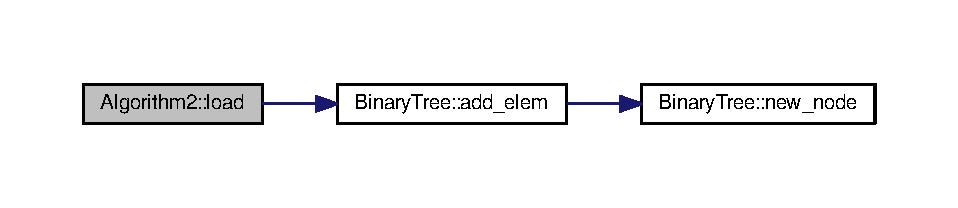
\includegraphics[width=350pt]{class_algorithm2_a50bbb4421660c4200dba66e9da9d7969_cgraph}
\end{center}
\end{figure}


\hypertarget{class_algorithm2_a409e58d5fb0b6d2407cc986cf163703b}{\index{Algorithm2@{Algorithm2}!run\-Algorithm@{run\-Algorithm}}
\index{run\-Algorithm@{run\-Algorithm}!Algorithm2@{Algorithm2}}
\subsubsection[{run\-Algorithm}]{\setlength{\rightskip}{0pt plus 5cm}void Algorithm2\-::run\-Algorithm (
\begin{DoxyParamCaption}
\item[{int}]{\-\_\-border}
\end{DoxyParamCaption}
)\hspace{0.3cm}{\ttfamily [virtual]}}}\label{class_algorithm2_a409e58d5fb0b6d2407cc986cf163703b}

\begin{DoxyParams}[1]{Parametry}
\mbox{\tt in}  & {\em \-\_\-border} & -\/ ilosc elementow dla ktorych algorytm ma wykonac swoje dzialanie. \\
\hline
\end{DoxyParams}


Implementuje \hyperlink{class_benchmark_a33e60395b1e126ca65c3aea3abf6debf}{Benchmark}.



Definicja w linii 22 pliku algorithm2.\-cpp.



Oto graf wywołań dla tej funkcji\-:\nopagebreak
\begin{figure}[H]
\begin{center}
\leavevmode
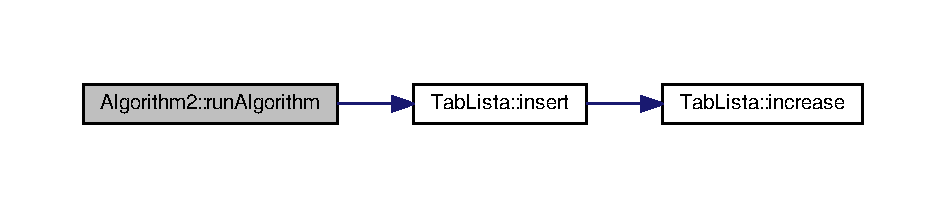
\includegraphics[width=350pt]{class_algorithm2_a409e58d5fb0b6d2407cc986cf163703b_cgraph}
\end{center}
\end{figure}


\hypertarget{class_algorithm2_a3d7e4d0c9308d0b97250cb5596a73165}{\index{Algorithm2@{Algorithm2}!unload@{unload}}
\index{unload@{unload}!Algorithm2@{Algorithm2}}
\subsubsection[{unload}]{\setlength{\rightskip}{0pt plus 5cm}void Algorithm2\-::unload (
\begin{DoxyParamCaption}
\item[{int}]{\-\_\-border}
\end{DoxyParamCaption}
)\hspace{0.3cm}{\ttfamily [virtual]}}}\label{class_algorithm2_a3d7e4d0c9308d0b97250cb5596a73165}

\begin{DoxyParams}[1]{Parametry}
\mbox{\tt in}  & {\em \-\_\-border} & -\/ ilosc elementow dla ktorych metoda ma wykonac swoje dzialanie. \\
\hline
\end{DoxyParams}


Implementuje \hyperlink{class_benchmark_a2dcfb6ee9e648ae88d8c131b2b191bed}{Benchmark}.



Definicja w linii 35 pliku algorithm2.\-cpp.



Oto graf wywołań dla tej funkcji\-:\nopagebreak
\begin{figure}[H]
\begin{center}
\leavevmode
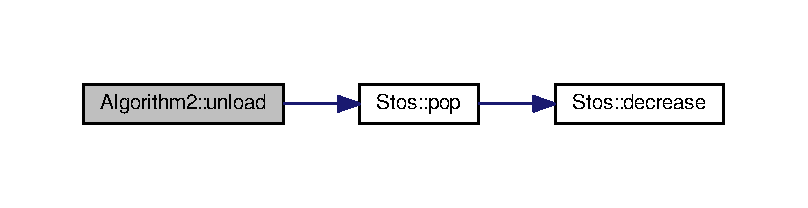
\includegraphics[width=350pt]{class_algorithm2_a3d7e4d0c9308d0b97250cb5596a73165_cgraph}
\end{center}
\end{figure}




\subsection{Dokumentacja atrybutów składowych}
\hypertarget{class_algorithm2_aff7c12a2dc0294d120a36ae0efc4af6a}{\index{Algorithm2@{Algorithm2}!tree@{tree}}
\index{tree@{tree}!Algorithm2@{Algorithm2}}
\subsubsection[{tree}]{\setlength{\rightskip}{0pt plus 5cm}{\bf Binary\-Tree} Algorithm2\-::tree\hspace{0.3cm}{\ttfamily [private]}}}\label{class_algorithm2_aff7c12a2dc0294d120a36ae0efc4af6a}


Definicja w linii 14 pliku algorithm2.\-hh.



Dokumentacja dla tej klasy została wygenerowana z plików\-:\begin{DoxyCompactItemize}
\item 
\hyperlink{algorithm2_8hh}{algorithm2.\-hh}\item 
\hyperlink{algorithm2_8cpp}{algorithm2.\-cpp}\end{DoxyCompactItemize}

\hypertarget{class_algorithm3}{\section{Dokumentacja klasy Algorithm3}
\label{class_algorithm3}\index{Algorithm3@{Algorithm3}}
}


Klasa \hyperlink{class_algorithm3}{Algorithm3} modelujaca algorytm sortowania stosu. Obiekt tego typu reprezentuje algorytm wykonujacy sortowanie szybkie na elementach stosu. Dziedziczy po klasie \hyperlink{class_benchmark}{Benchmark}.  




{\ttfamily \#include $<$algorithm3.\-hh$>$}



Diagram dziedziczenia dla Algorithm3
\nopagebreak
\begin{figure}[H]
\begin{center}
\leavevmode
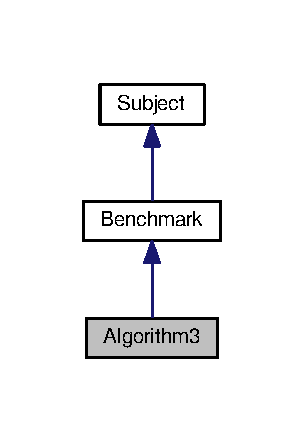
\includegraphics[width=146pt]{class_algorithm3__inherit__graph}
\end{center}
\end{figure}


Diagram współpracy dla Algorithm3\-:
\nopagebreak
\begin{figure}[H]
\begin{center}
\leavevmode
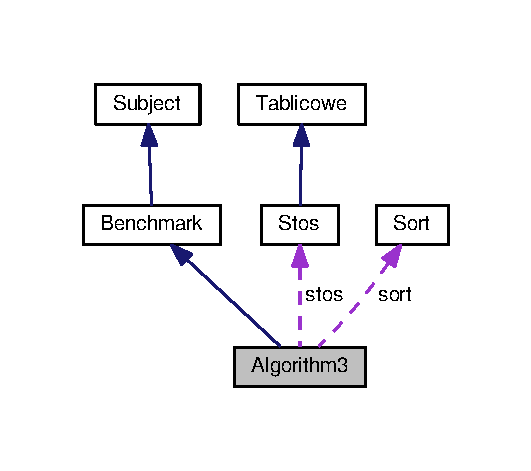
\includegraphics[width=255pt]{class_algorithm3__coll__graph}
\end{center}
\end{figure}
\subsection*{Metody publiczne}
\begin{DoxyCompactItemize}
\item 
\hyperlink{class_algorithm3_a88d9f8567616fd898bf202602726600d}{Algorithm3} ()
\begin{DoxyCompactList}\small\item\em Konstruktor obiektu \hyperlink{class_algorithm3}{Algorithm3}. \end{DoxyCompactList}\item 
\hyperlink{class_algorithm3_a71f0a79b028ae3c867321bcf19a45188}{Algorithm3} (unsigned short $\ast$\-\_\-tab, int \-\_\-id)
\begin{DoxyCompactList}\small\item\em Konstruktor parametryczny obiektu \hyperlink{class_algorithm3}{Algorithm3}. \end{DoxyCompactList}\item 
\hyperlink{class_algorithm3_ae9d1f5425fce3fc93d356fe8bf103e28}{$\sim$\-Algorithm3} ()
\begin{DoxyCompactList}\small\item\em Destruktor obiektu \hyperlink{class_algorithm3}{Algorithm3}. \end{DoxyCompactList}\item 
virtual void \hyperlink{class_algorithm3_a92b082327e99863c82981cdaec9a45a1}{load} (int \-\_\-border)
\begin{DoxyCompactList}\small\item\em Metoda przygotowywania algorytmu. Metoda sluzy do przygotowania warunkow do przeprowadzenia testu. \end{DoxyCompactList}\item 
virtual void \hyperlink{class_algorithm3_a170d77ee28866741214e65da7efcf533}{unload} (int \-\_\-border)
\begin{DoxyCompactList}\small\item\em Metoda sprzatania. Metoda sluzy do oproznienia struktury. \end{DoxyCompactList}\item 
virtual void \hyperlink{class_algorithm3_ac5c80b248190a12fa770e0386f694570}{run\-Algorithm} (int \-\_\-border)
\begin{DoxyCompactList}\small\item\em Metoda uruchamiania algorytmu. Metoda sluzy do wykonywania danego algorytmu. Sortuje elementy stosu. \end{DoxyCompactList}\end{DoxyCompactItemize}
\subsection*{Atrybuty prywatne}
\begin{DoxyCompactItemize}
\item 
\hyperlink{class_r_b_tree}{R\-B\-Tree} \hyperlink{class_algorithm3_a258233c4774afd7d6e6d5a1198955556}{tree}
\begin{DoxyCompactList}\small\item\em Zmienna przechowujaca drzewo czerwono-\/czarne. \end{DoxyCompactList}\end{DoxyCompactItemize}
\subsection*{Dodatkowe Dziedziczone Składowe}


\subsection{Opis szczegółowy}


Definicja w linii 10 pliku algorithm3.\-hh.



\subsection{Dokumentacja konstruktora i destruktora}
\hypertarget{class_algorithm3_a88d9f8567616fd898bf202602726600d}{\index{Algorithm3@{Algorithm3}!Algorithm3@{Algorithm3}}
\index{Algorithm3@{Algorithm3}!Algorithm3@{Algorithm3}}
\subsubsection[{Algorithm3}]{\setlength{\rightskip}{0pt plus 5cm}Algorithm3\-::\-Algorithm3 (
\begin{DoxyParamCaption}
{}
\end{DoxyParamCaption}
)\hspace{0.3cm}{\ttfamily [inline]}}}\label{class_algorithm3_a88d9f8567616fd898bf202602726600d}


Definicja w linii 20 pliku algorithm3.\-hh.

\hypertarget{class_algorithm3_a71f0a79b028ae3c867321bcf19a45188}{\index{Algorithm3@{Algorithm3}!Algorithm3@{Algorithm3}}
\index{Algorithm3@{Algorithm3}!Algorithm3@{Algorithm3}}
\subsubsection[{Algorithm3}]{\setlength{\rightskip}{0pt plus 5cm}Algorithm3\-::\-Algorithm3 (
\begin{DoxyParamCaption}
\item[{unsigned short $\ast$}]{\-\_\-tab, }
\item[{int}]{\-\_\-id}
\end{DoxyParamCaption}
)}}\label{class_algorithm3_a71f0a79b028ae3c867321bcf19a45188}

\begin{DoxyParams}[1]{Parametry}
\mbox{\tt in}  & {\em \-\_\-tab} & -\/ tablica przechowujaca dane wejsciowe. \\
\hline
\mbox{\tt in}  & {\em \-\_\-id} & -\/ identyfikator algorytmu. \\
\hline
\end{DoxyParams}


Definicja w linii 10 pliku algorithm3.\-cpp.

\hypertarget{class_algorithm3_ae9d1f5425fce3fc93d356fe8bf103e28}{\index{Algorithm3@{Algorithm3}!$\sim$\-Algorithm3@{$\sim$\-Algorithm3}}
\index{$\sim$\-Algorithm3@{$\sim$\-Algorithm3}!Algorithm3@{Algorithm3}}
\subsubsection[{$\sim$\-Algorithm3}]{\setlength{\rightskip}{0pt plus 5cm}Algorithm3\-::$\sim$\-Algorithm3 (
\begin{DoxyParamCaption}
{}
\end{DoxyParamCaption}
)}}\label{class_algorithm3_ae9d1f5425fce3fc93d356fe8bf103e28}


Definicja w linii 17 pliku algorithm3.\-cpp.



\subsection{Dokumentacja funkcji składowych}
\hypertarget{class_algorithm3_a92b082327e99863c82981cdaec9a45a1}{\index{Algorithm3@{Algorithm3}!load@{load}}
\index{load@{load}!Algorithm3@{Algorithm3}}
\subsubsection[{load}]{\setlength{\rightskip}{0pt plus 5cm}void Algorithm3\-::load (
\begin{DoxyParamCaption}
\item[{int}]{\-\_\-border}
\end{DoxyParamCaption}
)\hspace{0.3cm}{\ttfamily [virtual]}}}\label{class_algorithm3_a92b082327e99863c82981cdaec9a45a1}

\begin{DoxyParams}[1]{Parametry}
\mbox{\tt in}  & {\em \-\_\-border} & -\/ ilosc elementow dla ktorych metoda ma wykonac swoje dzialanie. \\
\hline
\end{DoxyParams}


Implementuje \hyperlink{class_benchmark_a41f66d36949f1488facb8e3d49c99f67}{Benchmark}.



Definicja w linii 29 pliku algorithm3.\-cpp.

\hypertarget{class_algorithm3_ac5c80b248190a12fa770e0386f694570}{\index{Algorithm3@{Algorithm3}!run\-Algorithm@{run\-Algorithm}}
\index{run\-Algorithm@{run\-Algorithm}!Algorithm3@{Algorithm3}}
\subsubsection[{run\-Algorithm}]{\setlength{\rightskip}{0pt plus 5cm}void Algorithm3\-::run\-Algorithm (
\begin{DoxyParamCaption}
\item[{int}]{\-\_\-border}
\end{DoxyParamCaption}
)\hspace{0.3cm}{\ttfamily [virtual]}}}\label{class_algorithm3_ac5c80b248190a12fa770e0386f694570}

\begin{DoxyParams}[1]{Parametry}
\mbox{\tt in}  & {\em \-\_\-border} & -\/ ilosc elementow dla ktorych algorytm ma wykonac swoje dzialanie. \\
\hline
\end{DoxyParams}


Implementuje \hyperlink{class_benchmark_a33e60395b1e126ca65c3aea3abf6debf}{Benchmark}.



Definicja w linii 22 pliku algorithm3.\-cpp.



Oto graf wywołań dla tej funkcji\-:
\nopagebreak
\begin{figure}[H]
\begin{center}
\leavevmode
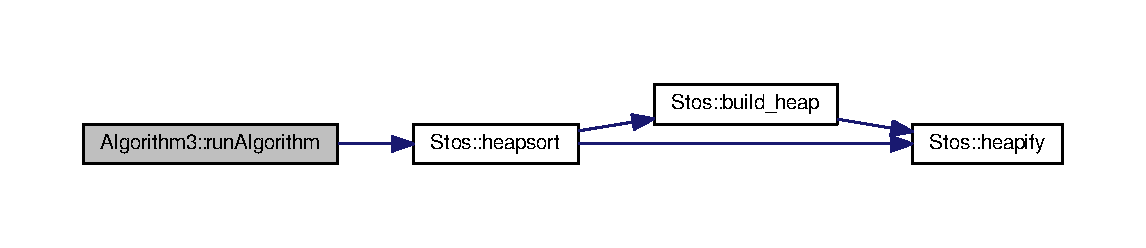
\includegraphics[width=350pt]{class_algorithm3_ac5c80b248190a12fa770e0386f694570_cgraph}
\end{center}
\end{figure}


\hypertarget{class_algorithm3_a170d77ee28866741214e65da7efcf533}{\index{Algorithm3@{Algorithm3}!unload@{unload}}
\index{unload@{unload}!Algorithm3@{Algorithm3}}
\subsubsection[{unload}]{\setlength{\rightskip}{0pt plus 5cm}void Algorithm3\-::unload (
\begin{DoxyParamCaption}
\item[{int}]{\-\_\-border}
\end{DoxyParamCaption}
)\hspace{0.3cm}{\ttfamily [virtual]}}}\label{class_algorithm3_a170d77ee28866741214e65da7efcf533}

\begin{DoxyParams}[1]{Parametry}
\mbox{\tt in}  & {\em \-\_\-border} & -\/ ilosc elementow dla ktorych metoda ma wykonac swoje dzialanie. \\
\hline
\end{DoxyParams}


Implementuje \hyperlink{class_benchmark_a2dcfb6ee9e648ae88d8c131b2b191bed}{Benchmark}.



Definicja w linii 34 pliku algorithm3.\-cpp.



Oto graf wywołań dla tej funkcji\-:
\nopagebreak
\begin{figure}[H]
\begin{center}
\leavevmode
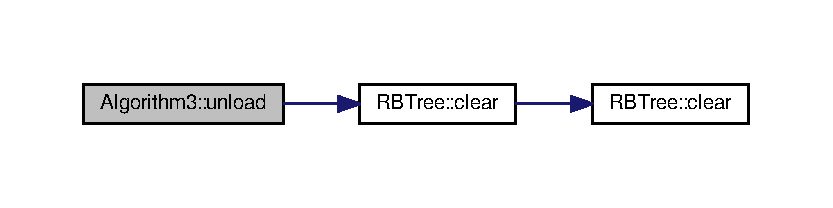
\includegraphics[width=350pt]{class_algorithm3_a170d77ee28866741214e65da7efcf533_cgraph}
\end{center}
\end{figure}




\subsection{Dokumentacja atrybutów składowych}
\hypertarget{class_algorithm3_a258233c4774afd7d6e6d5a1198955556}{\index{Algorithm3@{Algorithm3}!tree@{tree}}
\index{tree@{tree}!Algorithm3@{Algorithm3}}
\subsubsection[{tree}]{\setlength{\rightskip}{0pt plus 5cm}{\bf R\-B\-Tree} Algorithm3\-::tree\hspace{0.3cm}{\ttfamily [private]}}}\label{class_algorithm3_a258233c4774afd7d6e6d5a1198955556}


Definicja w linii 14 pliku algorithm3.\-hh.



Dokumentacja dla tej klasy została wygenerowana z plików\-:\begin{DoxyCompactItemize}
\item 
\hyperlink{algorithm3_8hh}{algorithm3.\-hh}\item 
\hyperlink{algorithm3_8cpp}{algorithm3.\-cpp}\end{DoxyCompactItemize}

\hypertarget{class_algorithm4}{\section{Dokumentacja klasy Algorithm4}
\label{class_algorithm4}\index{Algorithm4@{Algorithm4}}
}


Klasa \hyperlink{class_algorithm4}{Algorithm4} modelujaca algorytm sortowania stosu. Obiekt tego typu reprezentuje algorytm wykonujacy sortowanie szybkie po optymalizacji na elementach stosu. Dziedziczy po klasie \hyperlink{class_benchmark}{Benchmark}.  




{\ttfamily \#include $<$algorithm4.\-hh$>$}



Diagram dziedziczenia dla Algorithm4\nopagebreak
\begin{figure}[H]
\begin{center}
\leavevmode
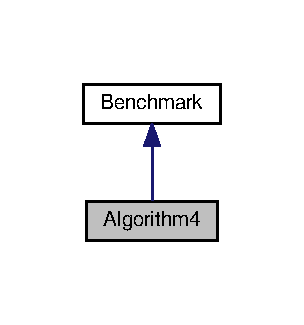
\includegraphics[width=146pt]{class_algorithm4__inherit__graph}
\end{center}
\end{figure}


Diagram współpracy dla Algorithm4\-:\nopagebreak
\begin{figure}[H]
\begin{center}
\leavevmode
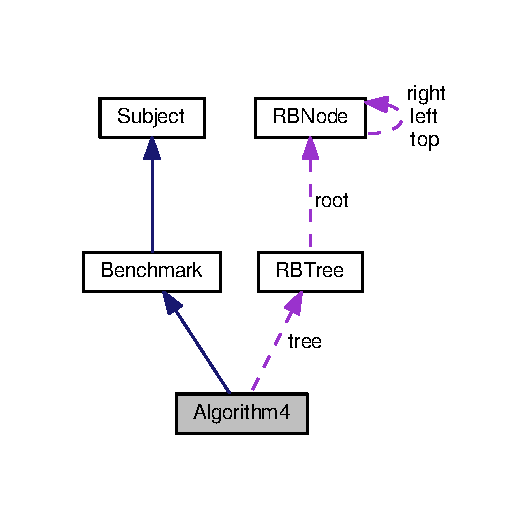
\includegraphics[width=255pt]{class_algorithm4__coll__graph}
\end{center}
\end{figure}
\subsection*{Metody publiczne}
\begin{DoxyCompactItemize}
\item 
\hyperlink{class_algorithm4_a79f0bdede29ae14437031022b7a32278}{Algorithm4} ()
\begin{DoxyCompactList}\small\item\em Konstruktor obiektu \hyperlink{class_algorithm4}{Algorithm4}. \end{DoxyCompactList}\item 
\hyperlink{class_algorithm4_a7e9812499c980dfc9e2032d1a3728b09}{Algorithm4} (unsigned short $\ast$\-\_\-tab, int \-\_\-id)
\begin{DoxyCompactList}\small\item\em Konstruktor parametryczny obiektu \hyperlink{class_algorithm4}{Algorithm4}. \end{DoxyCompactList}\item 
\hyperlink{class_algorithm4_ad73b6bd1ca2b289db737e3e4f5b40abf}{$\sim$\-Algorithm4} ()
\begin{DoxyCompactList}\small\item\em Destruktor obiektu \hyperlink{class_algorithm4}{Algorithm4}. \end{DoxyCompactList}\item 
virtual void \hyperlink{class_algorithm4_aa86adbf6be3052692f885c1be28b2300}{load} (int \-\_\-border)
\begin{DoxyCompactList}\small\item\em Metoda przygotowywania algorytmu. Metoda sluzy do przygotowania warunkow do przeprowadzenia testu. \end{DoxyCompactList}\item 
virtual void \hyperlink{class_algorithm4_a673e2d2373378ab01a7f0378d978f162}{unload} (int \-\_\-border)
\begin{DoxyCompactList}\small\item\em Metoda sprzatania. Metoda sluzy do oproznienia struktury. \end{DoxyCompactList}\item 
virtual void \hyperlink{class_algorithm4_ad1e715e2d6ddec7607f3cafa77443cd2}{run\-Algorithm} (int \-\_\-border)
\begin{DoxyCompactList}\small\item\em Metoda uruchamiania algorytmu. Metoda sluzy do wykonywania danego algorytmu. Sortuje elementy stosu. \end{DoxyCompactList}\end{DoxyCompactItemize}
\subsection*{Atrybuty prywatne}
\begin{DoxyCompactItemize}
\item 
\hyperlink{struct_stos}{Stos} \hyperlink{class_algorithm4_aa9946110dc906caed6ddc49c60f7a3c8}{stos}
\begin{DoxyCompactList}\small\item\em Zmienna przechowujaca stos. \end{DoxyCompactList}\item 
\hyperlink{class_sort}{Sort} \hyperlink{class_algorithm4_afbc43ff18fc5837d95e5746353bfc54a}{sort}
\begin{DoxyCompactList}\small\item\em Zmienna przechowujaca klase sortujaca. \end{DoxyCompactList}\end{DoxyCompactItemize}
\subsection*{Dodatkowe Dziedziczone Składowe}


\subsection{Opis szczegółowy}


Definicja w linii 10 pliku algorithm4.\-hh.



\subsection{Dokumentacja konstruktora i destruktora}
\hypertarget{class_algorithm4_a79f0bdede29ae14437031022b7a32278}{\index{Algorithm4@{Algorithm4}!Algorithm4@{Algorithm4}}
\index{Algorithm4@{Algorithm4}!Algorithm4@{Algorithm4}}
\subsubsection[{Algorithm4}]{\setlength{\rightskip}{0pt plus 5cm}Algorithm4\-::\-Algorithm4 (
\begin{DoxyParamCaption}
{}
\end{DoxyParamCaption}
)\hspace{0.3cm}{\ttfamily [inline]}}}\label{class_algorithm4_a79f0bdede29ae14437031022b7a32278}


Definicja w linii 24 pliku algorithm4.\-hh.

\hypertarget{class_algorithm4_a7e9812499c980dfc9e2032d1a3728b09}{\index{Algorithm4@{Algorithm4}!Algorithm4@{Algorithm4}}
\index{Algorithm4@{Algorithm4}!Algorithm4@{Algorithm4}}
\subsubsection[{Algorithm4}]{\setlength{\rightskip}{0pt plus 5cm}Algorithm4\-::\-Algorithm4 (
\begin{DoxyParamCaption}
\item[{unsigned short $\ast$}]{\-\_\-tab, }
\item[{int}]{\-\_\-id}
\end{DoxyParamCaption}
)}}\label{class_algorithm4_a7e9812499c980dfc9e2032d1a3728b09}

\begin{DoxyParams}[1]{Parametry}
\mbox{\tt in}  & {\em \-\_\-tab} & -\/ tablica przechowujaca dane wejsciowe. \\
\hline
\mbox{\tt in}  & {\em \-\_\-id} & -\/ identyfikator algorytmu. \\
\hline
\end{DoxyParams}


Definicja w linii 12 pliku algorithm4.\-cpp.

\hypertarget{class_algorithm4_ad73b6bd1ca2b289db737e3e4f5b40abf}{\index{Algorithm4@{Algorithm4}!$\sim$\-Algorithm4@{$\sim$\-Algorithm4}}
\index{$\sim$\-Algorithm4@{$\sim$\-Algorithm4}!Algorithm4@{Algorithm4}}
\subsubsection[{$\sim$\-Algorithm4}]{\setlength{\rightskip}{0pt plus 5cm}Algorithm4\-::$\sim$\-Algorithm4 (
\begin{DoxyParamCaption}
{}
\end{DoxyParamCaption}
)}}\label{class_algorithm4_ad73b6bd1ca2b289db737e3e4f5b40abf}


Definicja w linii 19 pliku algorithm4.\-cpp.



\subsection{Dokumentacja funkcji składowych}
\hypertarget{class_algorithm4_aa86adbf6be3052692f885c1be28b2300}{\index{Algorithm4@{Algorithm4}!load@{load}}
\index{load@{load}!Algorithm4@{Algorithm4}}
\subsubsection[{load}]{\setlength{\rightskip}{0pt plus 5cm}void Algorithm4\-::load (
\begin{DoxyParamCaption}
\item[{int}]{\-\_\-border}
\end{DoxyParamCaption}
)\hspace{0.3cm}{\ttfamily [virtual]}}}\label{class_algorithm4_aa86adbf6be3052692f885c1be28b2300}

\begin{DoxyParams}[1]{Parametry}
\mbox{\tt in}  & {\em \-\_\-border} & -\/ ilosc elementow dla ktorych metoda ma wykonac swoje dzialanie. \\
\hline
\end{DoxyParams}


Implementuje \hyperlink{class_benchmark_a41f66d36949f1488facb8e3d49c99f67}{Benchmark}.



Definicja w linii 30 pliku algorithm4.\-cpp.



Oto graf wywołań dla tej funkcji\-:\nopagebreak
\begin{figure}[H]
\begin{center}
\leavevmode
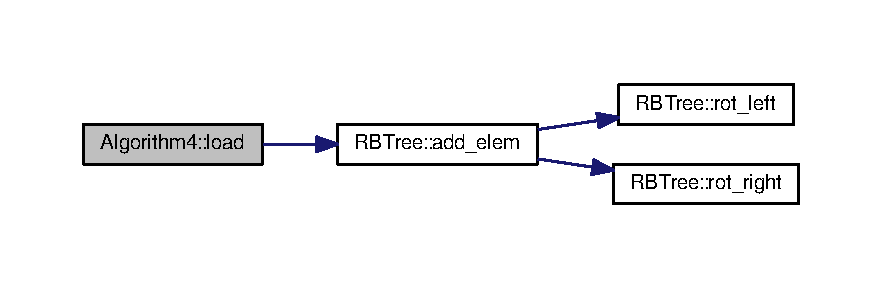
\includegraphics[width=350pt]{class_algorithm4_aa86adbf6be3052692f885c1be28b2300_cgraph}
\end{center}
\end{figure}


\hypertarget{class_algorithm4_ad1e715e2d6ddec7607f3cafa77443cd2}{\index{Algorithm4@{Algorithm4}!run\-Algorithm@{run\-Algorithm}}
\index{run\-Algorithm@{run\-Algorithm}!Algorithm4@{Algorithm4}}
\subsubsection[{run\-Algorithm}]{\setlength{\rightskip}{0pt plus 5cm}void Algorithm4\-::run\-Algorithm (
\begin{DoxyParamCaption}
\item[{int}]{\-\_\-border}
\end{DoxyParamCaption}
)\hspace{0.3cm}{\ttfamily [virtual]}}}\label{class_algorithm4_ad1e715e2d6ddec7607f3cafa77443cd2}

\begin{DoxyParams}[1]{Parametry}
\mbox{\tt in}  & {\em \-\_\-border} & -\/ ilosc elementow dla ktorych algorytm ma wykonac swoje dzialanie. \\
\hline
\end{DoxyParams}


Implementuje \hyperlink{class_benchmark_a33e60395b1e126ca65c3aea3abf6debf}{Benchmark}.



Definicja w linii 24 pliku algorithm4.\-cpp.



Oto graf wywołań dla tej funkcji\-:\nopagebreak
\begin{figure}[H]
\begin{center}
\leavevmode
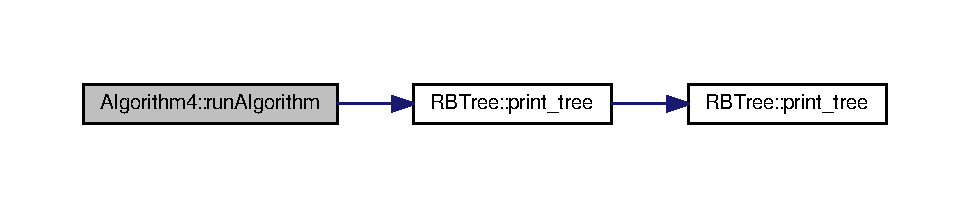
\includegraphics[width=322pt]{class_algorithm4_ad1e715e2d6ddec7607f3cafa77443cd2_cgraph}
\end{center}
\end{figure}


\hypertarget{class_algorithm4_a673e2d2373378ab01a7f0378d978f162}{\index{Algorithm4@{Algorithm4}!unload@{unload}}
\index{unload@{unload}!Algorithm4@{Algorithm4}}
\subsubsection[{unload}]{\setlength{\rightskip}{0pt plus 5cm}void Algorithm4\-::unload (
\begin{DoxyParamCaption}
\item[{int}]{\-\_\-border}
\end{DoxyParamCaption}
)\hspace{0.3cm}{\ttfamily [virtual]}}}\label{class_algorithm4_a673e2d2373378ab01a7f0378d978f162}

\begin{DoxyParams}[1]{Parametry}
\mbox{\tt in}  & {\em \-\_\-border} & -\/ ilosc elementow dla ktorych metoda ma wykonac swoje dzialanie. \\
\hline
\end{DoxyParams}


Implementuje \hyperlink{class_benchmark_a2dcfb6ee9e648ae88d8c131b2b191bed}{Benchmark}.



Definicja w linii 36 pliku algorithm4.\-cpp.



Oto graf wywołań dla tej funkcji\-:\nopagebreak
\begin{figure}[H]
\begin{center}
\leavevmode
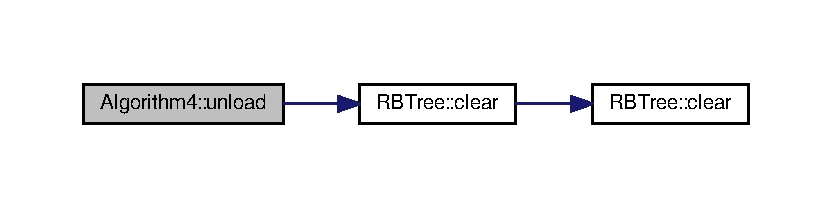
\includegraphics[width=350pt]{class_algorithm4_a673e2d2373378ab01a7f0378d978f162_cgraph}
\end{center}
\end{figure}




\subsection{Dokumentacja atrybutów składowych}
\hypertarget{class_algorithm4_afbc43ff18fc5837d95e5746353bfc54a}{\index{Algorithm4@{Algorithm4}!sort@{sort}}
\index{sort@{sort}!Algorithm4@{Algorithm4}}
\subsubsection[{sort}]{\setlength{\rightskip}{0pt plus 5cm}{\bf Sort} Algorithm4\-::sort\hspace{0.3cm}{\ttfamily [private]}}}\label{class_algorithm4_afbc43ff18fc5837d95e5746353bfc54a}


Definicja w linii 18 pliku algorithm4.\-hh.

\hypertarget{class_algorithm4_aa9946110dc906caed6ddc49c60f7a3c8}{\index{Algorithm4@{Algorithm4}!stos@{stos}}
\index{stos@{stos}!Algorithm4@{Algorithm4}}
\subsubsection[{stos}]{\setlength{\rightskip}{0pt plus 5cm}{\bf Stos} Algorithm4\-::stos\hspace{0.3cm}{\ttfamily [private]}}}\label{class_algorithm4_aa9946110dc906caed6ddc49c60f7a3c8}


Definicja w linii 14 pliku algorithm4.\-hh.



Dokumentacja dla tej klasy została wygenerowana z plików\-:\begin{DoxyCompactItemize}
\item 
\hyperlink{algorithm4_8hh}{algorithm4.\-hh}\item 
\hyperlink{algorithm4_8cpp}{algorithm4.\-cpp}\end{DoxyCompactItemize}

\hypertarget{struct_a_node}{\section{Dokumentacja struktury A\-Node}
\label{struct_a_node}\index{A\-Node@{A\-Node}}
}


Struktura \hyperlink{struct_a_node}{A\-Node}. Obiekt tego typu reprezentuje pojedyncza komorke wraz ze wskaznikiem na nastepna komorke listy.  




{\ttfamily \#include $<$asocjacyjna.\-hh$>$}



Diagram współpracy dla A\-Node\-:
\nopagebreak
\begin{figure}[H]
\begin{center}
\leavevmode
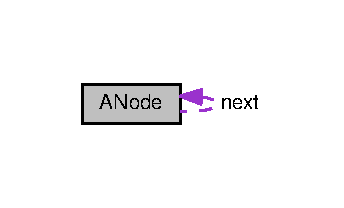
\includegraphics[width=165pt]{struct_a_node__coll__graph}
\end{center}
\end{figure}
\subsection*{Metody publiczne}
\begin{DoxyCompactItemize}
\item 
\hyperlink{struct_a_node_ad12f3f4440ad56e7e90d5ac927ba096a}{A\-Node} (const char $\ast$\-\_\-k)
\begin{DoxyCompactList}\small\item\em Konstruktor paramteryczny struktury \hyperlink{struct_a_node}{A\-Node}. \end{DoxyCompactList}\item 
\hyperlink{struct_a_node_a8fd9487184ba1af2150456919869cd60}{A\-Node} (const \hyperlink{struct_a_node}{A\-Node} \&\-\_\-s)
\begin{DoxyCompactList}\small\item\em Konstruktor paramteryczny struktury \hyperlink{struct_a_node}{A\-Node}. \end{DoxyCompactList}\item 
\hyperlink{struct_a_node_aec880ec60e95396aba5ffdc6ce0a4e8d}{$\sim$\-A\-Node} ()
\begin{DoxyCompactList}\small\item\em Destruktor struktury node. \end{DoxyCompactList}\end{DoxyCompactItemize}
\subsection*{Atrybuty publiczne}
\begin{DoxyCompactItemize}
\item 
\hyperlink{struct_a_node}{A\-Node} $\ast$ \hyperlink{struct_a_node_a97878d7354cd6beff5963e4fd0799805}{next}
\begin{DoxyCompactList}\small\item\em Wskaznik na nastepna komorke. \end{DoxyCompactList}\item 
char $\ast$ \hyperlink{struct_a_node_a3601f1eb35c094a209e3eab174f4afd4}{key}
\begin{DoxyCompactList}\small\item\em Wskaznik na klucz. \end{DoxyCompactList}\item 
int \hyperlink{struct_a_node_a4dbd8d8f9c7082fef7bc7f9113163301}{val}
\begin{DoxyCompactList}\small\item\em Wartosc klucza. \end{DoxyCompactList}\end{DoxyCompactItemize}
\subsection*{Metody prywatne}
\begin{DoxyCompactItemize}
\item 
\hyperlink{struct_a_node}{A\-Node} \& \hyperlink{struct_a_node_a96160014f2ca78c2b7baf21051752dbc}{operator=} (const \hyperlink{struct_a_node}{A\-Node} \&)
\begin{DoxyCompactList}\small\item\em Przeladowanie operatora przypisania. Zabezpieczenie przed automatycznym operatorem przypisania. \end{DoxyCompactList}\end{DoxyCompactItemize}


\subsection{Opis szczegółowy}


Definicja w linii 11 pliku asocjacyjna.\-hh.



\subsection{Dokumentacja konstruktora i destruktora}
\hypertarget{struct_a_node_ad12f3f4440ad56e7e90d5ac927ba096a}{\index{A\-Node@{A\-Node}!A\-Node@{A\-Node}}
\index{A\-Node@{A\-Node}!ANode@{A\-Node}}
\subsubsection[{A\-Node}]{\setlength{\rightskip}{0pt plus 5cm}A\-Node\-::\-A\-Node (
\begin{DoxyParamCaption}
\item[{const char $\ast$}]{\-\_\-k}
\end{DoxyParamCaption}
)}}\label{struct_a_node_ad12f3f4440ad56e7e90d5ac927ba096a}

\begin{DoxyParams}[1]{Parametry}
\mbox{\tt in}  & {\em \-\_\-k} & -\/ wskaznik na klucz. \\
\hline
\end{DoxyParams}


Definicja w linii 8 pliku asocjacyjna.\-cpp.

\hypertarget{struct_a_node_a8fd9487184ba1af2150456919869cd60}{\index{A\-Node@{A\-Node}!A\-Node@{A\-Node}}
\index{A\-Node@{A\-Node}!ANode@{A\-Node}}
\subsubsection[{A\-Node}]{\setlength{\rightskip}{0pt plus 5cm}A\-Node\-::\-A\-Node (
\begin{DoxyParamCaption}
\item[{const {\bf A\-Node} \&}]{\-\_\-s}
\end{DoxyParamCaption}
)}}\label{struct_a_node_a8fd9487184ba1af2150456919869cd60}

\begin{DoxyParams}[1]{Parametry}
\mbox{\tt in}  & {\em \-\_\-s} & -\/ referencja do pary klucz-\/wartosc. \\
\hline
\end{DoxyParams}


Definicja w linii 15 pliku asocjacyjna.\-cpp.

\hypertarget{struct_a_node_aec880ec60e95396aba5ffdc6ce0a4e8d}{\index{A\-Node@{A\-Node}!$\sim$\-A\-Node@{$\sim$\-A\-Node}}
\index{$\sim$\-A\-Node@{$\sim$\-A\-Node}!ANode@{A\-Node}}
\subsubsection[{$\sim$\-A\-Node}]{\setlength{\rightskip}{0pt plus 5cm}A\-Node\-::$\sim$\-A\-Node (
\begin{DoxyParamCaption}
{}
\end{DoxyParamCaption}
)}}\label{struct_a_node_aec880ec60e95396aba5ffdc6ce0a4e8d}


Definicja w linii 29 pliku asocjacyjna.\-cpp.



\subsection{Dokumentacja funkcji składowych}
\hypertarget{struct_a_node_a96160014f2ca78c2b7baf21051752dbc}{\index{A\-Node@{A\-Node}!operator=@{operator=}}
\index{operator=@{operator=}!ANode@{A\-Node}}
\subsubsection[{operator=}]{\setlength{\rightskip}{0pt plus 5cm}{\bf A\-Node}\& A\-Node\-::operator= (
\begin{DoxyParamCaption}
\item[{const {\bf A\-Node} \&}]{}
\end{DoxyParamCaption}
)\hspace{0.3cm}{\ttfamily [private]}}}\label{struct_a_node_a96160014f2ca78c2b7baf21051752dbc}


\subsection{Dokumentacja atrybutów składowych}
\hypertarget{struct_a_node_a3601f1eb35c094a209e3eab174f4afd4}{\index{A\-Node@{A\-Node}!key@{key}}
\index{key@{key}!ANode@{A\-Node}}
\subsubsection[{key}]{\setlength{\rightskip}{0pt plus 5cm}char$\ast$ A\-Node\-::key}}\label{struct_a_node_a3601f1eb35c094a209e3eab174f4afd4}


Definicja w linii 19 pliku asocjacyjna.\-hh.

\hypertarget{struct_a_node_a97878d7354cd6beff5963e4fd0799805}{\index{A\-Node@{A\-Node}!next@{next}}
\index{next@{next}!ANode@{A\-Node}}
\subsubsection[{next}]{\setlength{\rightskip}{0pt plus 5cm}{\bf A\-Node}$\ast$ A\-Node\-::next}}\label{struct_a_node_a97878d7354cd6beff5963e4fd0799805}


Definicja w linii 15 pliku asocjacyjna.\-hh.

\hypertarget{struct_a_node_a4dbd8d8f9c7082fef7bc7f9113163301}{\index{A\-Node@{A\-Node}!val@{val}}
\index{val@{val}!ANode@{A\-Node}}
\subsubsection[{val}]{\setlength{\rightskip}{0pt plus 5cm}int A\-Node\-::val}}\label{struct_a_node_a4dbd8d8f9c7082fef7bc7f9113163301}


Definicja w linii 23 pliku asocjacyjna.\-hh.



Dokumentacja dla tej struktury została wygenerowana z plików\-:\begin{DoxyCompactItemize}
\item 
\hyperlink{asocjacyjna_8hh}{asocjacyjna.\-hh}\item 
\hyperlink{asocjacyjna_8cpp}{asocjacyjna.\-cpp}\end{DoxyCompactItemize}

\hypertarget{class_asocjacyjna}{\section{Dokumentacja klasy Asocjacyjna}
\label{class_asocjacyjna}\index{Asocjacyjna@{Asocjacyjna}}
}


Klasa \hyperlink{class_asocjacyjna}{Asocjacyjna}. Obiekt tego typu reprezentuje strukture danych typu lista asocjacyjna wraz z operacjami mozliwymi do wykonania na tej strukturze.  




{\ttfamily \#include $<$asocjacyjna.\-hh$>$}



Diagram współpracy dla Asocjacyjna\-:\nopagebreak
\begin{figure}[H]
\begin{center}
\leavevmode
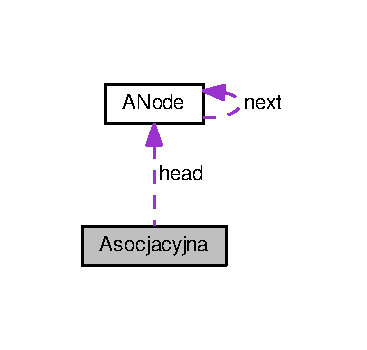
\includegraphics[width=176pt]{class_asocjacyjna__coll__graph}
\end{center}
\end{figure}
\subsection*{Metody publiczne}
\begin{DoxyCompactItemize}
\item 
\hyperlink{class_asocjacyjna_a1c65a8bcfb084dcdfa205b052fefd141}{Asocjacyjna} ()
\begin{DoxyCompactList}\small\item\em Konstruktor bezparametryczny obiektu \hyperlink{class_asocjacyjna}{Asocjacyjna}. \end{DoxyCompactList}\item 
\hyperlink{class_asocjacyjna_a4dfb11269865e38b988dbacf1cc44409}{Asocjacyjna} (const \hyperlink{class_asocjacyjna}{Asocjacyjna} \&l)
\begin{DoxyCompactList}\small\item\em Konstruktor paramteryczny obiektu \hyperlink{class_asocjacyjna}{Asocjacyjna}. \end{DoxyCompactList}\item 
\hyperlink{class_asocjacyjna}{Asocjacyjna} \& \hyperlink{class_asocjacyjna_add65b5482b856404b130b69b71a5cb9b}{operator=} (const \hyperlink{class_asocjacyjna}{Asocjacyjna} \&l)
\begin{DoxyCompactList}\small\item\em Przeladowanie operatora przypisania. Sluzy do wstawiania do klasy elementow innego obiektu tego samego typu. \end{DoxyCompactList}\item 
\hyperlink{class_asocjacyjna_aa33745fa9b42796199d58f29fa0cd8f0}{$\sim$\-Asocjacyjna} ()
\begin{DoxyCompactList}\small\item\em Destruktor obiektu Komorka. \end{DoxyCompactList}\item 
int \& \hyperlink{class_asocjacyjna_a517bf91bf5550a58669c61ec4e209a8a}{operator\mbox{[}$\,$\mbox{]}} (const char $\ast$key)
\begin{DoxyCompactList}\small\item\em Przeladowanie operatora nawiasu kwadratowego. Sluzy do wpisywania klucza oraz wartosci. \end{DoxyCompactList}\end{DoxyCompactItemize}
\subsection*{Metody chronione}
\begin{DoxyCompactItemize}
\item 
void \hyperlink{class_asocjacyjna_a9209f79af7b566f327c8c83f6b879f8b}{clear} ()
\begin{DoxyCompactList}\small\item\em Metoda usuwania zawartosci listy. \end{DoxyCompactList}\item 
\hyperlink{struct_a_node}{A\-Node} $\ast$ \hyperlink{class_asocjacyjna_a98eefccd8a668d6589d35bea37a811a1}{find} (const char $\ast$key) const 
\begin{DoxyCompactList}\small\item\em Metoda wyszukiwania elementu o podanym kluczu. \end{DoxyCompactList}\item 
void \hyperlink{class_asocjacyjna_a0c4f5e81b3998cde7c677c658c949d83}{insert} (const char $\ast$key, int value)
\begin{DoxyCompactList}\small\item\em Metoda wstawiania nowej pary klucz-\/wartosc. \end{DoxyCompactList}\item 
void \hyperlink{class_asocjacyjna_a92d60b9a27bddb7e13ea358db62f684e}{swap} (\hyperlink{class_asocjacyjna}{Asocjacyjna} \&l)
\begin{DoxyCompactList}\small\item\em Metoda zamiany dwoch list. \end{DoxyCompactList}\end{DoxyCompactItemize}
\subsection*{Atrybuty prywatne}
\begin{DoxyCompactItemize}
\item 
\hyperlink{struct_a_node}{A\-Node} $\ast$ \hyperlink{class_asocjacyjna_adf1a2a6a5b0b6254122050bbe8c69046}{head}
\begin{DoxyCompactList}\small\item\em Wskaznik na pierwsza pare klucz-\/wartosc. \end{DoxyCompactList}\end{DoxyCompactItemize}
\subsection*{Przyjaciele}
\begin{DoxyCompactItemize}
\item 
std\-::ostream \& \hyperlink{class_asocjacyjna_ac80cff774adfcde4838393e913a2c059}{operator$<$$<$} (std\-::ostream \&stream, \hyperlink{class_asocjacyjna}{Asocjacyjna} \&l)
\begin{DoxyCompactList}\small\item\em Przeladowanie operatora przesuniecia bitowego. Sluzy do wypisywania zawartosci listy na strumien wyjsciowy. \end{DoxyCompactList}\end{DoxyCompactItemize}


\subsection{Opis szczegółowy}


Definicja w linii 74 pliku asocjacyjna.\-hh.



\subsection{Dokumentacja konstruktora i destruktora}
\hypertarget{class_asocjacyjna_a1c65a8bcfb084dcdfa205b052fefd141}{\index{Asocjacyjna@{Asocjacyjna}!Asocjacyjna@{Asocjacyjna}}
\index{Asocjacyjna@{Asocjacyjna}!Asocjacyjna@{Asocjacyjna}}
\subsubsection[{Asocjacyjna}]{\setlength{\rightskip}{0pt plus 5cm}Asocjacyjna\-::\-Asocjacyjna (
\begin{DoxyParamCaption}
{}
\end{DoxyParamCaption}
)}}\label{class_asocjacyjna_a1c65a8bcfb084dcdfa205b052fefd141}


Definicja w linii 8 pliku asocjacyjna.\-cpp.

\hypertarget{class_asocjacyjna_a4dfb11269865e38b988dbacf1cc44409}{\index{Asocjacyjna@{Asocjacyjna}!Asocjacyjna@{Asocjacyjna}}
\index{Asocjacyjna@{Asocjacyjna}!Asocjacyjna@{Asocjacyjna}}
\subsubsection[{Asocjacyjna}]{\setlength{\rightskip}{0pt plus 5cm}Asocjacyjna\-::\-Asocjacyjna (
\begin{DoxyParamCaption}
\item[{const {\bf Asocjacyjna} \&}]{l}
\end{DoxyParamCaption}
)}}\label{class_asocjacyjna_a4dfb11269865e38b988dbacf1cc44409}

\begin{DoxyParams}[1]{Parametry}
\mbox{\tt in}  & {\em l} & -\/ referencja do listy. \\
\hline
\end{DoxyParams}


Definicja w linii 14 pliku asocjacyjna.\-cpp.



Oto graf wywołań dla tej funkcji\-:\nopagebreak
\begin{figure}[H]
\begin{center}
\leavevmode
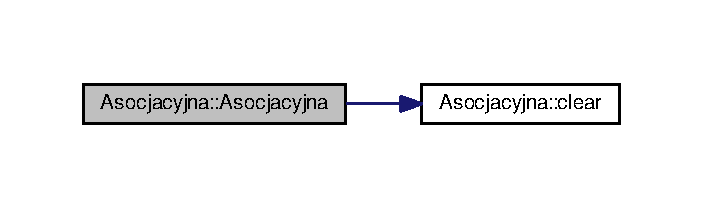
\includegraphics[width=338pt]{class_asocjacyjna_a4dfb11269865e38b988dbacf1cc44409_cgraph}
\end{center}
\end{figure}


\hypertarget{class_asocjacyjna_aa33745fa9b42796199d58f29fa0cd8f0}{\index{Asocjacyjna@{Asocjacyjna}!$\sim$\-Asocjacyjna@{$\sim$\-Asocjacyjna}}
\index{$\sim$\-Asocjacyjna@{$\sim$\-Asocjacyjna}!Asocjacyjna@{Asocjacyjna}}
\subsubsection[{$\sim$\-Asocjacyjna}]{\setlength{\rightskip}{0pt plus 5cm}Asocjacyjna\-::$\sim$\-Asocjacyjna (
\begin{DoxyParamCaption}
{}
\end{DoxyParamCaption}
)}}\label{class_asocjacyjna_aa33745fa9b42796199d58f29fa0cd8f0}


Definicja w linii 38 pliku asocjacyjna.\-cpp.



Oto graf wywołań dla tej funkcji\-:\nopagebreak
\begin{figure}[H]
\begin{center}
\leavevmode
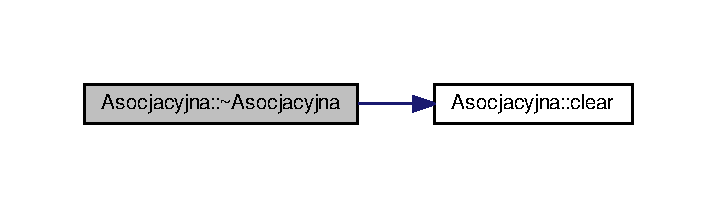
\includegraphics[width=344pt]{class_asocjacyjna_aa33745fa9b42796199d58f29fa0cd8f0_cgraph}
\end{center}
\end{figure}




\subsection{Dokumentacja funkcji składowych}
\hypertarget{class_asocjacyjna_a9209f79af7b566f327c8c83f6b879f8b}{\index{Asocjacyjna@{Asocjacyjna}!clear@{clear}}
\index{clear@{clear}!Asocjacyjna@{Asocjacyjna}}
\subsubsection[{clear}]{\setlength{\rightskip}{0pt plus 5cm}void Asocjacyjna\-::clear (
\begin{DoxyParamCaption}
{}
\end{DoxyParamCaption}
)\hspace{0.3cm}{\ttfamily [protected]}}}\label{class_asocjacyjna_a9209f79af7b566f327c8c83f6b879f8b}


Definicja w linii 73 pliku asocjacyjna.\-cpp.



Oto graf wywoływań tej funkcji\-:\nopagebreak
\begin{figure}[H]
\begin{center}
\leavevmode
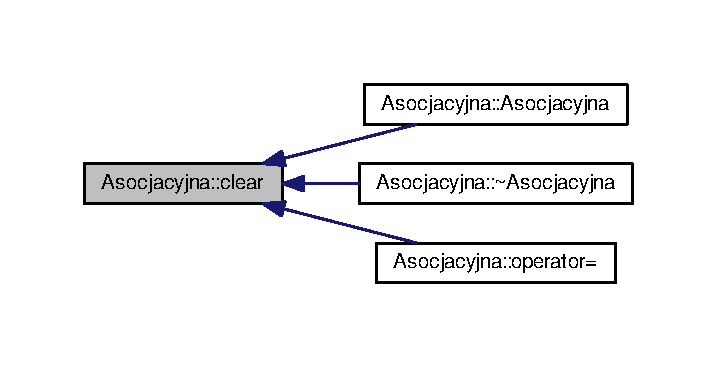
\includegraphics[width=344pt]{class_asocjacyjna_a9209f79af7b566f327c8c83f6b879f8b_icgraph}
\end{center}
\end{figure}


\hypertarget{class_asocjacyjna_a98eefccd8a668d6589d35bea37a811a1}{\index{Asocjacyjna@{Asocjacyjna}!find@{find}}
\index{find@{find}!Asocjacyjna@{Asocjacyjna}}
\subsubsection[{find}]{\setlength{\rightskip}{0pt plus 5cm}{\bf A\-Node} $\ast$ Asocjacyjna\-::find (
\begin{DoxyParamCaption}
\item[{const char $\ast$}]{key}
\end{DoxyParamCaption}
) const\hspace{0.3cm}{\ttfamily [protected]}}}\label{class_asocjacyjna_a98eefccd8a668d6589d35bea37a811a1}

\begin{DoxyParams}[1]{Parametry}
\mbox{\tt in}  & {\em key} & -\/ wskaznik na wyszukiwany klucz. \\
\hline
\end{DoxyParams}
\begin{DoxyReturn}{Zwraca}
wskaznik na szukana pare klucz-\/wartosc, nullprt gdy nie znalezniono klucza. 
\end{DoxyReturn}


Definicja w linii 101 pliku asocjacyjna.\-cpp.



Oto graf wywoływań tej funkcji\-:\nopagebreak
\begin{figure}[H]
\begin{center}
\leavevmode
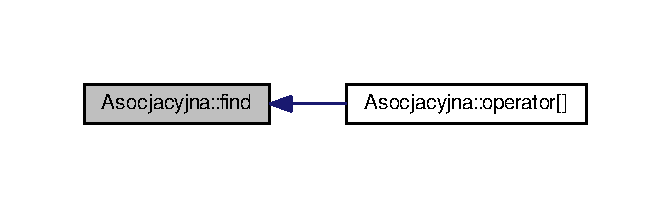
\includegraphics[width=322pt]{class_asocjacyjna_a98eefccd8a668d6589d35bea37a811a1_icgraph}
\end{center}
\end{figure}


\hypertarget{class_asocjacyjna_a0c4f5e81b3998cde7c677c658c949d83}{\index{Asocjacyjna@{Asocjacyjna}!insert@{insert}}
\index{insert@{insert}!Asocjacyjna@{Asocjacyjna}}
\subsubsection[{insert}]{\setlength{\rightskip}{0pt plus 5cm}void Asocjacyjna\-::insert (
\begin{DoxyParamCaption}
\item[{const char $\ast$}]{key, }
\item[{int}]{value}
\end{DoxyParamCaption}
)\hspace{0.3cm}{\ttfamily [protected]}}}\label{class_asocjacyjna_a0c4f5e81b3998cde7c677c658c949d83}

\begin{DoxyParams}[1]{Parametry}
\mbox{\tt in}  & {\em key} & -\/ wskaznik na klucz. \\
\hline
\mbox{\tt in}  & {\em value} & -\/ wartosc klucza. \\
\hline
\end{DoxyParams}


Definicja w linii 84 pliku asocjacyjna.\-cpp.



Oto graf wywoływań tej funkcji\-:\nopagebreak
\begin{figure}[H]
\begin{center}
\leavevmode
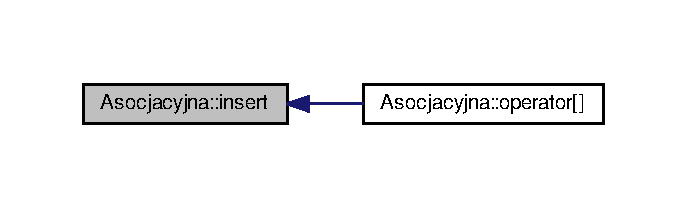
\includegraphics[width=330pt]{class_asocjacyjna_a0c4f5e81b3998cde7c677c658c949d83_icgraph}
\end{center}
\end{figure}


\hypertarget{class_asocjacyjna_add65b5482b856404b130b69b71a5cb9b}{\index{Asocjacyjna@{Asocjacyjna}!operator=@{operator=}}
\index{operator=@{operator=}!Asocjacyjna@{Asocjacyjna}}
\subsubsection[{operator=}]{\setlength{\rightskip}{0pt plus 5cm}{\bf Asocjacyjna} \& Asocjacyjna\-::operator= (
\begin{DoxyParamCaption}
\item[{const {\bf Asocjacyjna} \&}]{l}
\end{DoxyParamCaption}
)}}\label{class_asocjacyjna_add65b5482b856404b130b69b71a5cb9b}

\begin{DoxyParams}[1]{Parametry}
\mbox{\tt in}  & {\em l} & -\/ referencja do listy. \\
\hline
\end{DoxyParams}


Definicja w linii 44 pliku asocjacyjna.\-cpp.



Oto graf wywołań dla tej funkcji\-:\nopagebreak
\begin{figure}[H]
\begin{center}
\leavevmode
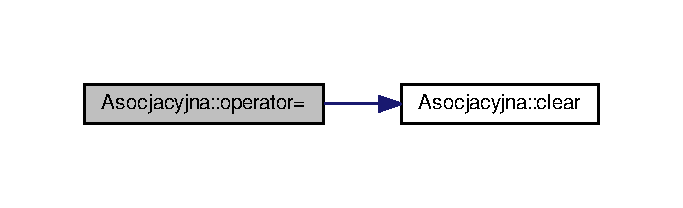
\includegraphics[width=328pt]{class_asocjacyjna_add65b5482b856404b130b69b71a5cb9b_cgraph}
\end{center}
\end{figure}


\hypertarget{class_asocjacyjna_a517bf91bf5550a58669c61ec4e209a8a}{\index{Asocjacyjna@{Asocjacyjna}!operator\mbox{[}$\,$\mbox{]}@{operator[]}}
\index{operator\mbox{[}$\,$\mbox{]}@{operator[]}!Asocjacyjna@{Asocjacyjna}}
\subsubsection[{operator[]}]{\setlength{\rightskip}{0pt plus 5cm}int \& Asocjacyjna\-::operator\mbox{[}$\,$\mbox{]} (
\begin{DoxyParamCaption}
\item[{const char $\ast$}]{key}
\end{DoxyParamCaption}
)}}\label{class_asocjacyjna_a517bf91bf5550a58669c61ec4e209a8a}

\begin{DoxyParams}[1]{Parametry}
\mbox{\tt in}  & {\em key} & -\/ wskaznik na klucz. \\
\hline
\end{DoxyParams}
\begin{DoxyReturn}{Zwraca}
wartosc klucza. 
\end{DoxyReturn}


Definicja w linii 114 pliku asocjacyjna.\-cpp.



Oto graf wywołań dla tej funkcji\-:\nopagebreak
\begin{figure}[H]
\begin{center}
\leavevmode
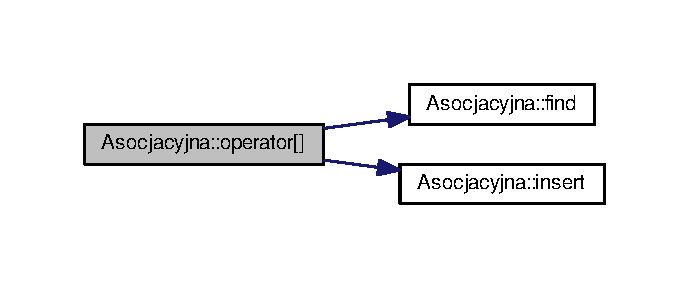
\includegraphics[width=330pt]{class_asocjacyjna_a517bf91bf5550a58669c61ec4e209a8a_cgraph}
\end{center}
\end{figure}


\hypertarget{class_asocjacyjna_a92d60b9a27bddb7e13ea358db62f684e}{\index{Asocjacyjna@{Asocjacyjna}!swap@{swap}}
\index{swap@{swap}!Asocjacyjna@{Asocjacyjna}}
\subsubsection[{swap}]{\setlength{\rightskip}{0pt plus 5cm}void Asocjacyjna\-::swap (
\begin{DoxyParamCaption}
\item[{{\bf Asocjacyjna} \&}]{l}
\end{DoxyParamCaption}
)\hspace{0.3cm}{\ttfamily [protected]}}}\label{class_asocjacyjna_a92d60b9a27bddb7e13ea358db62f684e}

\begin{DoxyParams}[1]{Parametry}
\mbox{\tt in}  & {\em l} & -\/ referencja do listy. \\
\hline
\end{DoxyParams}


Definicja w linii 93 pliku asocjacyjna.\-cpp.



\subsection{Dokumentacja przyjaciół i funkcji związanych}
\hypertarget{class_asocjacyjna_ac80cff774adfcde4838393e913a2c059}{\index{Asocjacyjna@{Asocjacyjna}!operator$<$$<$@{operator$<$$<$}}
\index{operator$<$$<$@{operator$<$$<$}!Asocjacyjna@{Asocjacyjna}}
\subsubsection[{operator$<$$<$}]{\setlength{\rightskip}{0pt plus 5cm}std\-::ostream\& operator$<$$<$ (
\begin{DoxyParamCaption}
\item[{std\-::ostream \&}]{stream, }
\item[{{\bf Asocjacyjna} \&}]{l}
\end{DoxyParamCaption}
)\hspace{0.3cm}{\ttfamily [friend]}}}\label{class_asocjacyjna_ac80cff774adfcde4838393e913a2c059}

\begin{DoxyParams}[1]{Parametry}
\mbox{\tt in}  & {\em stream} & -\/ referencja do strumienia wyjsciowego. \\
\hline
\mbox{\tt in}  & {\em l} & -\/ referencja do listy. \\
\hline
\end{DoxyParams}
\begin{DoxyReturn}{Zwraca}
strumien wyjsciowy. 
\end{DoxyReturn}


Definicja w linii 141 pliku asocjacyjna.\-hh.



\subsection{Dokumentacja atrybutów składowych}
\hypertarget{class_asocjacyjna_adf1a2a6a5b0b6254122050bbe8c69046}{\index{Asocjacyjna@{Asocjacyjna}!head@{head}}
\index{head@{head}!Asocjacyjna@{Asocjacyjna}}
\subsubsection[{head}]{\setlength{\rightskip}{0pt plus 5cm}{\bf A\-Node}$\ast$ Asocjacyjna\-::head\hspace{0.3cm}{\ttfamily [private]}}}\label{class_asocjacyjna_adf1a2a6a5b0b6254122050bbe8c69046}


Definicja w linii 79 pliku asocjacyjna.\-hh.



Dokumentacja dla tej klasy została wygenerowana z plików\-:\begin{DoxyCompactItemize}
\item 
\hyperlink{asocjacyjna_8hh}{asocjacyjna.\-hh}\item 
\hyperlink{asocjacyjna_8cpp}{asocjacyjna.\-cpp}\end{DoxyCompactItemize}

\hypertarget{class_benchmark}{\section{Dokumentacja klasy Benchmark}
\label{class_benchmark}\index{Benchmark@{Benchmark}}
}


Klasa \hyperlink{class_benchmark}{Benchmark} modelujaca program benchmarkujacy. Obiekt tego typu reprezentuje program sprawdzajacy szybkosc wykonywania algorytmow.  




{\ttfamily \#include $<$benchmark.\-hh$>$}



Diagram dziedziczenia dla Benchmark\nopagebreak
\begin{figure}[H]
\begin{center}
\leavevmode
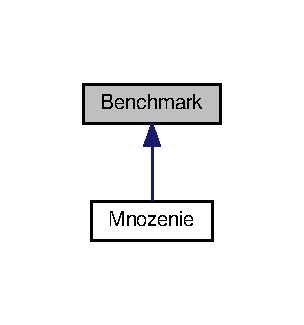
\includegraphics[width=350pt]{class_benchmark__inherit__graph}
\end{center}
\end{figure}
\subsection*{Metody publiczne}
\begin{DoxyCompactItemize}
\item 
\hyperlink{class_benchmark_acfca497989836a688d44477802e822d8}{Benchmark} ()
\begin{DoxyCompactList}\small\item\em Konstrukor obiektu \hyperlink{class_benchmark}{Benchmark}. \end{DoxyCompactList}\item 
\hyperlink{class_benchmark_a20476e07f09e2b20ed3e9a7f13a570e6}{$\sim$\-Benchmark} ()
\begin{DoxyCompactList}\small\item\em Destruktor obiektu \hyperlink{class_benchmark}{Benchmark}. \end{DoxyCompactList}\item 
virtual void \hyperlink{class_benchmark_a900bc0d26c2ed6aa45afe4d5b295ccd1}{test\-Algorithm} (\hyperlink{class_benchmark}{Benchmark} $\ast$\-\_\-algorithm, int \-\_\-n) const 
\begin{DoxyCompactList}\small\item\em Metoda testowania algorytmu. Metoda sluzy to testowania szybkosci dzialania algorytmu. Wykonuje testowany algorytm dla 5 kolejnych ilosci elementow. Wykonanie algorytmu dla danego zestawu liczb powtarza dwa razy i usrednia wynik. Otrzymany czas wraz z iloscia testowanych danych zapisuje w pliku ret\-\_\-data.\-txt. \end{DoxyCompactList}\item 
virtual void \hyperlink{class_benchmark_a6363894c058e8bfe146de09d7126b29c}{run\-Algorithm} (int \-\_\-border)
\begin{DoxyCompactList}\small\item\em Metoda uruchamiania algorytmu. Metoda sluzy do wykonywania danego algorytmu. W klasie \hyperlink{class_benchmark}{Benchmark} nie ma konkretnego dzialania. \end{DoxyCompactList}\end{DoxyCompactItemize}
\subsection*{Atrybuty prywatne}
\begin{DoxyCompactItemize}
\item 
std\-::string \hyperlink{class_benchmark_aee0beda65009e7334d34c5957f78c49a}{nazwy} \mbox{[}4\mbox{]} = \{\char`\"{}ret\-\_\-data1.\-txt\char`\"{}, \char`\"{}ret\-\_\-data2.\-txt\char`\"{}, \char`\"{}ret\-\_\-data3.\-txt\char`\"{}, \char`\"{}ret\-\_\-data4.\-txt\char`\"{}\}
\begin{DoxyCompactList}\small\item\em Tablica stringow przechowujaca nazwy plikow do zapisu. \end{DoxyCompactList}\end{DoxyCompactItemize}


\subsection{Opis szczegółowy}


Definicja w linii 11 pliku benchmark.\-hh.



\subsection{Dokumentacja konstruktora i destruktora}
\hypertarget{class_benchmark_acfca497989836a688d44477802e822d8}{\index{Benchmark@{Benchmark}!Benchmark@{Benchmark}}
\index{Benchmark@{Benchmark}!Benchmark@{Benchmark}}
\subsubsection[{Benchmark}]{\setlength{\rightskip}{0pt plus 5cm}Benchmark\-::\-Benchmark (
\begin{DoxyParamCaption}
{}
\end{DoxyParamCaption}
)\hspace{0.3cm}{\ttfamily [inline]}}}\label{class_benchmark_acfca497989836a688d44477802e822d8}


Definicja w linii 23 pliku benchmark.\-hh.

\hypertarget{class_benchmark_a20476e07f09e2b20ed3e9a7f13a570e6}{\index{Benchmark@{Benchmark}!$\sim$\-Benchmark@{$\sim$\-Benchmark}}
\index{$\sim$\-Benchmark@{$\sim$\-Benchmark}!Benchmark@{Benchmark}}
\subsubsection[{$\sim$\-Benchmark}]{\setlength{\rightskip}{0pt plus 5cm}Benchmark\-::$\sim$\-Benchmark (
\begin{DoxyParamCaption}
{}
\end{DoxyParamCaption}
)\hspace{0.3cm}{\ttfamily [inline]}}}\label{class_benchmark_a20476e07f09e2b20ed3e9a7f13a570e6}


Definicja w linii 28 pliku benchmark.\-hh.



\subsection{Dokumentacja funkcji składowych}
\hypertarget{class_benchmark_a6363894c058e8bfe146de09d7126b29c}{\index{Benchmark@{Benchmark}!run\-Algorithm@{run\-Algorithm}}
\index{run\-Algorithm@{run\-Algorithm}!Benchmark@{Benchmark}}
\subsubsection[{run\-Algorithm}]{\setlength{\rightskip}{0pt plus 5cm}virtual void Benchmark\-::run\-Algorithm (
\begin{DoxyParamCaption}
\item[{int}]{\-\_\-border}
\end{DoxyParamCaption}
)\hspace{0.3cm}{\ttfamily [inline]}, {\ttfamily [virtual]}}}\label{class_benchmark_a6363894c058e8bfe146de09d7126b29c}

\begin{DoxyParams}[1]{Parametry}
\mbox{\tt in}  & {\em \-\_\-border} & -\/ ilosc elementow dla ktorych algorytm ma wykonac swoje dzialanie. \\
\hline
\end{DoxyParams}


Reimplementowana w \hyperlink{class_algorithm2_a409e58d5fb0b6d2407cc986cf163703b}{Algorithm2}, \hyperlink{class_algorithm_kolejka_ae9da3f1862fd90feb4a3c1d6b4f3dd8d}{Algorithm\-Kolejka}, \hyperlink{class_algorithm_lista_a5c41dbbd3ae7a9ac34edec1a51bc8eb1}{Algorithm\-Lista} i \hyperlink{class_algorithm_stos_a889f7150ae3651b40e5acca7542dbbd1}{Algorithm\-Stos}.



Definicja w linii 48 pliku benchmark.\-hh.



Oto graf wywoływań tej funkcji\-:\nopagebreak
\begin{figure}[H]
\begin{center}
\leavevmode
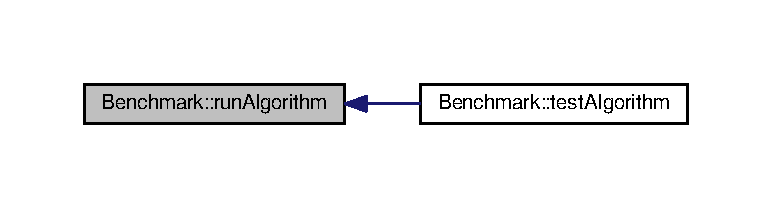
\includegraphics[width=350pt]{class_benchmark_a6363894c058e8bfe146de09d7126b29c_icgraph}
\end{center}
\end{figure}


\hypertarget{class_benchmark_a900bc0d26c2ed6aa45afe4d5b295ccd1}{\index{Benchmark@{Benchmark}!test\-Algorithm@{test\-Algorithm}}
\index{test\-Algorithm@{test\-Algorithm}!Benchmark@{Benchmark}}
\subsubsection[{test\-Algorithm}]{\setlength{\rightskip}{0pt plus 5cm}void Benchmark\-::test\-Algorithm (
\begin{DoxyParamCaption}
\item[{{\bf Benchmark} $\ast$}]{\-\_\-algorithm, }
\item[{int}]{\-\_\-n}
\end{DoxyParamCaption}
) const\hspace{0.3cm}{\ttfamily [virtual]}}}\label{class_benchmark_a900bc0d26c2ed6aa45afe4d5b295ccd1}

\begin{DoxyParams}[1]{Parametry}
\mbox{\tt in}  & {\em \-\_\-algorithm} & -\/ testowany algorytm. \\
\hline
\mbox{\tt in}  & {\em \-\_\-n} & -\/ indeks nazwy pliku \\
\hline
\end{DoxyParams}


Definicja w linii 12 pliku benchmark.\-cpp.



Oto graf wywołań dla tej funkcji\-:\nopagebreak
\begin{figure}[H]
\begin{center}
\leavevmode
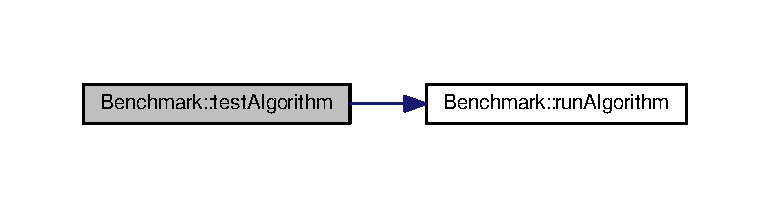
\includegraphics[width=350pt]{class_benchmark_a900bc0d26c2ed6aa45afe4d5b295ccd1_cgraph}
\end{center}
\end{figure}




\subsection{Dokumentacja atrybutów składowych}
\hypertarget{class_benchmark_aee0beda65009e7334d34c5957f78c49a}{\index{Benchmark@{Benchmark}!nazwy@{nazwy}}
\index{nazwy@{nazwy}!Benchmark@{Benchmark}}
\subsubsection[{nazwy}]{\setlength{\rightskip}{0pt plus 5cm}std\-::string Benchmark\-::nazwy\mbox{[}4\mbox{]} = \{\char`\"{}ret\-\_\-data1.\-txt\char`\"{}, \char`\"{}ret\-\_\-data2.\-txt\char`\"{}, \char`\"{}ret\-\_\-data3.\-txt\char`\"{}, \char`\"{}ret\-\_\-data4.\-txt\char`\"{}\}\hspace{0.3cm}{\ttfamily [private]}}}\label{class_benchmark_aee0beda65009e7334d34c5957f78c49a}


Definicja w linii 16 pliku benchmark.\-hh.



Dokumentacja dla tej klasy została wygenerowana z plików\-:\begin{DoxyCompactItemize}
\item 
\hyperlink{benchmark_8hh}{benchmark.\-hh}\item 
\hyperlink{benchmark_8cpp}{benchmark.\-cpp}\end{DoxyCompactItemize}

\hypertarget{class_kolejka}{\section{Dokumentacja klasy Kolejka}
\label{class_kolejka}\index{Kolejka@{Kolejka}}
}


Klasa \hyperlink{class_kolejka}{Kolejka} modelujaca strukture danych typu kolejka. Obiekt tego typu reprezentuje strukture danych typu kolejka wraz z operacjami mozliwymi do wykonania na tej strukturze. Dziedziczy po klasie \hyperlink{class_tablicowe}{Tablicowe}.  




{\ttfamily \#include $<$kolejka.\-hh$>$}



Diagram dziedziczenia dla Kolejka\nopagebreak
\begin{figure}[H]
\begin{center}
\leavevmode
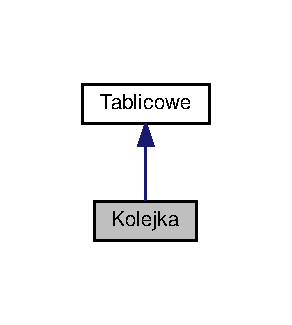
\includegraphics[width=140pt]{class_kolejka__inherit__graph}
\end{center}
\end{figure}


Diagram współpracy dla Kolejka\-:\nopagebreak
\begin{figure}[H]
\begin{center}
\leavevmode
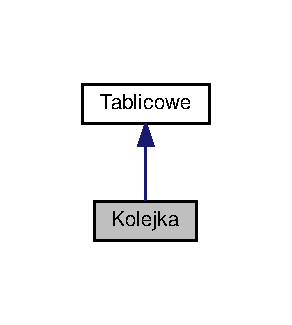
\includegraphics[width=140pt]{class_kolejka__coll__graph}
\end{center}
\end{figure}
\subsection*{Metody publiczne}
\begin{DoxyCompactItemize}
\item 
\hyperlink{class_kolejka_a37c886fdc73dce62b04da0381dec5484}{Kolejka} ()
\begin{DoxyCompactList}\small\item\em Konstruktor obiektu \hyperlink{class_kolejka}{Kolejka}. Tworzy kolejke o domyslnym rozmiarze rownym 8. \end{DoxyCompactList}\item 
\hyperlink{class_kolejka_ac942cc97bf0d2c30d11611c406acc5a8}{Kolejka} (long \-\_\-size)
\begin{DoxyCompactList}\small\item\em Konstruktor parametryczny obiektu \hyperlink{class_kolejka}{Kolejka}. Tworzy kolejke o zadanym rozmiarze rownym \-\_\-size. \end{DoxyCompactList}\item 
\hyperlink{class_kolejka_a352f86ff08cd47be6c35c60bb0f873a6}{$\sim$\-Kolejka} ()
\begin{DoxyCompactList}\small\item\em Destruktor obiektu \hyperlink{class_kolejka}{Kolejka}. \end{DoxyCompactList}\item 
void \hyperlink{class_kolejka_a8f3b0111e85f517d9eadb8ce996d4471}{enqueue} (int \-\_\-elem)
\begin{DoxyCompactList}\small\item\em Metoda dodawnia elementu. Metoda sluzy do dodawania elementu do kolejki. \end{DoxyCompactList}\item 
int \hyperlink{class_kolejka_af23261614bcf242a1934a99688a2debc}{dequeue} ()
\begin{DoxyCompactList}\small\item\em Metoda usuwania elementu. Metoda sluzy do usuwania elementu z kolejki. \end{DoxyCompactList}\end{DoxyCompactItemize}
\subsection*{Metody prywatne}
\begin{DoxyCompactItemize}
\item 
void \hyperlink{class_kolejka_ab4f51f0ec7fef36a85af6cfd1c257427}{increase} ()
\begin{DoxyCompactList}\small\item\em Metoda powiekszania kolejki. Metoda ta zwieksza ilosc pol w kolejce dwukrotnie. \end{DoxyCompactList}\item 
int \hyperlink{class_kolejka_acff09ebfbec69b06c91203bab30d815d}{decrease} ()
\begin{DoxyCompactList}\small\item\em Metoda pomniejszania kolejki. Metoda ta odejmuje od kolejki jedno pole. \end{DoxyCompactList}\end{DoxyCompactItemize}
\subsection*{Dodatkowe Dziedziczone Składowe}


\subsection{Opis szczegółowy}


Definicja w linii 10 pliku kolejka.\-hh.



\subsection{Dokumentacja konstruktora i destruktora}
\hypertarget{class_kolejka_a37c886fdc73dce62b04da0381dec5484}{\index{Kolejka@{Kolejka}!Kolejka@{Kolejka}}
\index{Kolejka@{Kolejka}!Kolejka@{Kolejka}}
\subsubsection[{Kolejka}]{\setlength{\rightskip}{0pt plus 5cm}Kolejka\-::\-Kolejka (
\begin{DoxyParamCaption}
{}
\end{DoxyParamCaption}
)}}\label{class_kolejka_a37c886fdc73dce62b04da0381dec5484}


Definicja w linii 7 pliku kolejka.\-cpp.

\hypertarget{class_kolejka_ac942cc97bf0d2c30d11611c406acc5a8}{\index{Kolejka@{Kolejka}!Kolejka@{Kolejka}}
\index{Kolejka@{Kolejka}!Kolejka@{Kolejka}}
\subsubsection[{Kolejka}]{\setlength{\rightskip}{0pt plus 5cm}Kolejka\-::\-Kolejka (
\begin{DoxyParamCaption}
\item[{long}]{\-\_\-size}
\end{DoxyParamCaption}
)}}\label{class_kolejka_ac942cc97bf0d2c30d11611c406acc5a8}

\begin{DoxyParams}[1]{Parametry}
\mbox{\tt in}  & {\em \-\_\-size} & -\/ startowy rozmiar struktury. \\
\hline
\end{DoxyParams}


Definicja w linii 17 pliku kolejka.\-cpp.

\hypertarget{class_kolejka_a352f86ff08cd47be6c35c60bb0f873a6}{\index{Kolejka@{Kolejka}!$\sim$\-Kolejka@{$\sim$\-Kolejka}}
\index{$\sim$\-Kolejka@{$\sim$\-Kolejka}!Kolejka@{Kolejka}}
\subsubsection[{$\sim$\-Kolejka}]{\setlength{\rightskip}{0pt plus 5cm}Kolejka\-::$\sim$\-Kolejka (
\begin{DoxyParamCaption}
{}
\end{DoxyParamCaption}
)}}\label{class_kolejka_a352f86ff08cd47be6c35c60bb0f873a6}


Definicja w linii 27 pliku kolejka.\-cpp.



\subsection{Dokumentacja funkcji składowych}
\hypertarget{class_kolejka_acff09ebfbec69b06c91203bab30d815d}{\index{Kolejka@{Kolejka}!decrease@{decrease}}
\index{decrease@{decrease}!Kolejka@{Kolejka}}
\subsubsection[{decrease}]{\setlength{\rightskip}{0pt plus 5cm}int Kolejka\-::decrease (
\begin{DoxyParamCaption}
{}
\end{DoxyParamCaption}
)\hspace{0.3cm}{\ttfamily [private]}}}\label{class_kolejka_acff09ebfbec69b06c91203bab30d815d}


Definicja w linii 45 pliku kolejka.\-cpp.



Oto graf wywoływań tej funkcji\-:\nopagebreak
\begin{figure}[H]
\begin{center}
\leavevmode
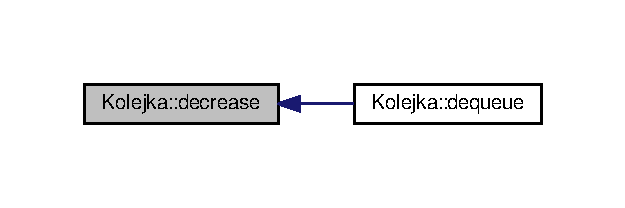
\includegraphics[width=300pt]{class_kolejka_acff09ebfbec69b06c91203bab30d815d_icgraph}
\end{center}
\end{figure}


\hypertarget{class_kolejka_af23261614bcf242a1934a99688a2debc}{\index{Kolejka@{Kolejka}!dequeue@{dequeue}}
\index{dequeue@{dequeue}!Kolejka@{Kolejka}}
\subsubsection[{dequeue}]{\setlength{\rightskip}{0pt plus 5cm}int Kolejka\-::dequeue (
\begin{DoxyParamCaption}
{}
\end{DoxyParamCaption}
)}}\label{class_kolejka_af23261614bcf242a1934a99688a2debc}
\begin{DoxyReturn}{Zwraca}
usuwany element. 
\end{DoxyReturn}


Definicja w linii 69 pliku kolejka.\-cpp.



Oto graf wywołań dla tej funkcji\-:\nopagebreak
\begin{figure}[H]
\begin{center}
\leavevmode
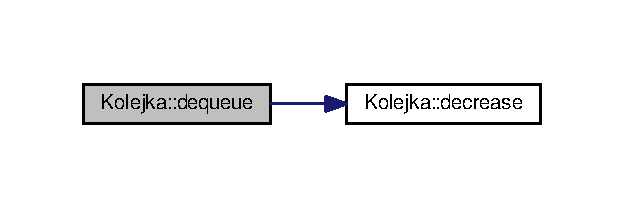
\includegraphics[width=300pt]{class_kolejka_af23261614bcf242a1934a99688a2debc_cgraph}
\end{center}
\end{figure}


\hypertarget{class_kolejka_a8f3b0111e85f517d9eadb8ce996d4471}{\index{Kolejka@{Kolejka}!enqueue@{enqueue}}
\index{enqueue@{enqueue}!Kolejka@{Kolejka}}
\subsubsection[{enqueue}]{\setlength{\rightskip}{0pt plus 5cm}void Kolejka\-::enqueue (
\begin{DoxyParamCaption}
\item[{int}]{\-\_\-elem}
\end{DoxyParamCaption}
)}}\label{class_kolejka_a8f3b0111e85f517d9eadb8ce996d4471}

\begin{DoxyParams}[1]{Parametry}
\mbox{\tt in}  & {\em \-\_\-elem} & -\/ dodawany element. \\
\hline
\end{DoxyParams}


Definicja w linii 60 pliku kolejka.\-cpp.



Oto graf wywołań dla tej funkcji\-:\nopagebreak
\begin{figure}[H]
\begin{center}
\leavevmode
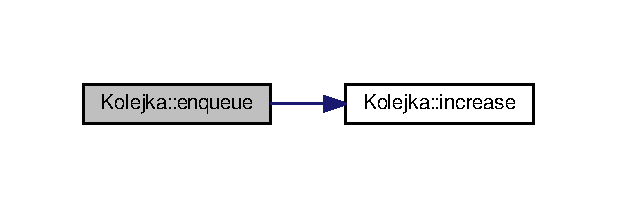
\includegraphics[width=296pt]{class_kolejka_a8f3b0111e85f517d9eadb8ce996d4471_cgraph}
\end{center}
\end{figure}


\hypertarget{class_kolejka_ab4f51f0ec7fef36a85af6cfd1c257427}{\index{Kolejka@{Kolejka}!increase@{increase}}
\index{increase@{increase}!Kolejka@{Kolejka}}
\subsubsection[{increase}]{\setlength{\rightskip}{0pt plus 5cm}void Kolejka\-::increase (
\begin{DoxyParamCaption}
{}
\end{DoxyParamCaption}
)\hspace{0.3cm}{\ttfamily [private]}}}\label{class_kolejka_ab4f51f0ec7fef36a85af6cfd1c257427}


Definicja w linii 33 pliku kolejka.\-cpp.



Oto graf wywoływań tej funkcji\-:\nopagebreak
\begin{figure}[H]
\begin{center}
\leavevmode
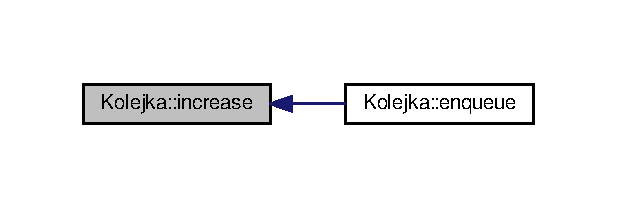
\includegraphics[width=296pt]{class_kolejka_ab4f51f0ec7fef36a85af6cfd1c257427_icgraph}
\end{center}
\end{figure}




Dokumentacja dla tej klasy została wygenerowana z plików\-:\begin{DoxyCompactItemize}
\item 
\hyperlink{kolejka_8hh}{kolejka.\-hh}\item 
\hyperlink{kolejka_8cpp}{kolejka.\-cpp}\end{DoxyCompactItemize}

\hypertarget{struct_lista_1_1_komorka}{\section{Dokumentacja struktury Lista\-:\-:Komorka}
\label{struct_lista_1_1_komorka}\index{Lista\-::\-Komorka@{Lista\-::\-Komorka}}
}


Struktura \hyperlink{struct_lista_1_1_komorka}{Komorka}. Obiekt tego typu reprezentuje pojedyncza komorke wraz ze wskaznikiem na nastepna komorke listy.  




Diagram współpracy dla Lista\-:\-:Komorka\-:\nopagebreak
\begin{figure}[H]
\begin{center}
\leavevmode
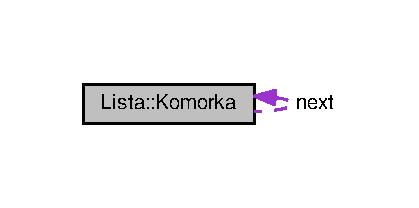
\includegraphics[width=201pt]{struct_lista_1_1_komorka__coll__graph}
\end{center}
\end{figure}
\subsection*{Metody publiczne}
\begin{DoxyCompactItemize}
\item 
\hyperlink{struct_lista_1_1_komorka_a1843c3c4ae9752cea90cfa21076f3e9c}{Komorka} (int \-\_\-elem)
\begin{DoxyCompactList}\small\item\em Konstruktor paramteryczny obiektu \hyperlink{struct_lista_1_1_komorka}{Komorka}. \end{DoxyCompactList}\item 
\hyperlink{struct_lista_1_1_komorka_a91f3a7f9bd8ebe05fa0821e1d989c506}{$\sim$\-Komorka} ()
\end{DoxyCompactItemize}
\subsection*{Atrybuty publiczne}
\begin{DoxyCompactItemize}
\item 
int \hyperlink{struct_lista_1_1_komorka_aeb683e1dce8a8c096cc54a6645137411}{elem}
\begin{DoxyCompactList}\small\item\em Wartosc elementu w pojedynczej komorce. \end{DoxyCompactList}\item 
\hyperlink{struct_lista_1_1_komorka}{Komorka} $\ast$ \hyperlink{struct_lista_1_1_komorka_aa04e9d2ed0260f2adbff6855f7bcd77e}{next}
\begin{DoxyCompactList}\small\item\em Wskaznik na nastepna komorke listy. \end{DoxyCompactList}\end{DoxyCompactItemize}


\subsection{Opis szczegółowy}


Definicja w linii 16 pliku lista.\-hh.



\subsection{Dokumentacja konstruktora i destruktora}
\hypertarget{struct_lista_1_1_komorka_a1843c3c4ae9752cea90cfa21076f3e9c}{\index{Lista\-::\-Komorka@{Lista\-::\-Komorka}!Komorka@{Komorka}}
\index{Komorka@{Komorka}!Lista::Komorka@{Lista\-::\-Komorka}}
\subsubsection[{Komorka}]{\setlength{\rightskip}{0pt plus 5cm}Lista\-::\-Komorka\-::\-Komorka (
\begin{DoxyParamCaption}
\item[{int}]{\-\_\-elem}
\end{DoxyParamCaption}
)\hspace{0.3cm}{\ttfamily [inline]}}}\label{struct_lista_1_1_komorka_a1843c3c4ae9752cea90cfa21076f3e9c}

\begin{DoxyParams}[1]{Parametry}
\mbox{\tt in}  & {\em \-\_\-elem} & -\/ wartosc przechowywanego elementu. \\
\hline
\end{DoxyParams}


Definicja w linii 29 pliku lista.\-hh.

\hypertarget{struct_lista_1_1_komorka_a91f3a7f9bd8ebe05fa0821e1d989c506}{\index{Lista\-::\-Komorka@{Lista\-::\-Komorka}!$\sim$\-Komorka@{$\sim$\-Komorka}}
\index{$\sim$\-Komorka@{$\sim$\-Komorka}!Lista::Komorka@{Lista\-::\-Komorka}}
\subsubsection[{$\sim$\-Komorka}]{\setlength{\rightskip}{0pt plus 5cm}Lista\-::\-Komorka\-::$\sim$\-Komorka (
\begin{DoxyParamCaption}
{}
\end{DoxyParamCaption}
)\hspace{0.3cm}{\ttfamily [inline]}}}\label{struct_lista_1_1_komorka_a91f3a7f9bd8ebe05fa0821e1d989c506}


Definicja w linii 33 pliku lista.\-hh.



\subsection{Dokumentacja atrybutów składowych}
\hypertarget{struct_lista_1_1_komorka_aeb683e1dce8a8c096cc54a6645137411}{\index{Lista\-::\-Komorka@{Lista\-::\-Komorka}!elem@{elem}}
\index{elem@{elem}!Lista::Komorka@{Lista\-::\-Komorka}}
\subsubsection[{elem}]{\setlength{\rightskip}{0pt plus 5cm}int Lista\-::\-Komorka\-::elem}}\label{struct_lista_1_1_komorka_aeb683e1dce8a8c096cc54a6645137411}


Definicja w linii 20 pliku lista.\-hh.

\hypertarget{struct_lista_1_1_komorka_aa04e9d2ed0260f2adbff6855f7bcd77e}{\index{Lista\-::\-Komorka@{Lista\-::\-Komorka}!next@{next}}
\index{next@{next}!Lista::Komorka@{Lista\-::\-Komorka}}
\subsubsection[{next}]{\setlength{\rightskip}{0pt plus 5cm}{\bf Komorka}$\ast$ Lista\-::\-Komorka\-::next}}\label{struct_lista_1_1_komorka_aa04e9d2ed0260f2adbff6855f7bcd77e}


Definicja w linii 24 pliku lista.\-hh.



Dokumentacja dla tej struktury została wygenerowana z pliku\-:\begin{DoxyCompactItemize}
\item 
\hyperlink{lista_8hh}{lista.\-hh}\end{DoxyCompactItemize}

\hypertarget{class_lista}{\section{Dokumentacja klasy Lista}
\label{class_lista}\index{Lista@{Lista}}
}


Klasa \hyperlink{class_lista}{Lista} modelujaca strukture danych typu lista. Obiekt tego typu reprezentuje strukture danych typu lista wraz z operacjami mozliwymi do wykonania na tej strukturze.  




{\ttfamily \#include $<$lista.\-hh$>$}



Diagram współpracy dla Lista\-:\nopagebreak
\begin{figure}[H]
\begin{center}
\leavevmode
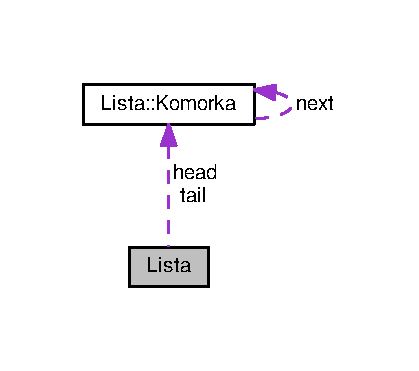
\includegraphics[width=201pt]{class_lista__coll__graph}
\end{center}
\end{figure}
\subsection*{Komponenty}
\begin{DoxyCompactItemize}
\item 
struct \hyperlink{struct_lista_1_1_komorka}{Komorka}
\begin{DoxyCompactList}\small\item\em Struktura \hyperlink{struct_lista_1_1_komorka}{Komorka}. Obiekt tego typu reprezentuje pojedyncza komorke wraz ze wskaznikiem na nastepna komorke listy. \end{DoxyCompactList}\end{DoxyCompactItemize}
\subsection*{Metody publiczne}
\begin{DoxyCompactItemize}
\item 
\hyperlink{class_lista_a1f668b36909182ef1360b48503529a31}{Lista} ()
\begin{DoxyCompactList}\small\item\em Konstruktor obiektu \hyperlink{class_lista}{Lista}. \end{DoxyCompactList}\item 
\hyperlink{class_lista_a4d7394b2728a00ad8404965b2e15d096}{$\sim$\-Lista} ()
\begin{DoxyCompactList}\small\item\em Destruktor obiektu \hyperlink{class_lista}{Lista}. \end{DoxyCompactList}\item 
void \hyperlink{class_lista_acec8ac807da644d8250c3c6043a208e1}{insert} (int \-\_\-elem)
\begin{DoxyCompactList}\small\item\em Metoda dodawnia elementu. Metoda sluzy do dodawania elementu do konca listy. \end{DoxyCompactList}\item 
void \hyperlink{class_lista_aa30ec43a5b51a0e37ffe8f098c5dcaa8}{remove} (int \-\_\-f)
\begin{DoxyCompactList}\small\item\em Metoda usuwania elementu. Metoda sluzy do usuwania elementu o wskazanym indeksie. \end{DoxyCompactList}\end{DoxyCompactItemize}
\subsection*{Atrybuty prywatne}
\begin{DoxyCompactItemize}
\item 
\hyperlink{struct_lista_1_1_komorka}{Komorka} $\ast$ \hyperlink{class_lista_aeba20505030183d334971bd44c3c8b95}{head}
\begin{DoxyCompactList}\small\item\em Wskaznik na poczatek listy. \end{DoxyCompactList}\item 
\hyperlink{struct_lista_1_1_komorka}{Komorka} $\ast$ \hyperlink{class_lista_a7d42e5f99e945d97c29d6f764f71f4e7}{tail}
\begin{DoxyCompactList}\small\item\em Wskaznik na koniec listy. \end{DoxyCompactList}\end{DoxyCompactItemize}


\subsection{Opis szczegółowy}


Definicja w linii 9 pliku lista.\-hh.



\subsection{Dokumentacja konstruktora i destruktora}
\hypertarget{class_lista_a1f668b36909182ef1360b48503529a31}{\index{Lista@{Lista}!Lista@{Lista}}
\index{Lista@{Lista}!Lista@{Lista}}
\subsubsection[{Lista}]{\setlength{\rightskip}{0pt plus 5cm}Lista\-::\-Lista (
\begin{DoxyParamCaption}
{}
\end{DoxyParamCaption}
)\hspace{0.3cm}{\ttfamily [inline]}}}\label{class_lista_a1f668b36909182ef1360b48503529a31}


Definicja w linii 49 pliku lista.\-hh.

\hypertarget{class_lista_a4d7394b2728a00ad8404965b2e15d096}{\index{Lista@{Lista}!$\sim$\-Lista@{$\sim$\-Lista}}
\index{$\sim$\-Lista@{$\sim$\-Lista}!Lista@{Lista}}
\subsubsection[{$\sim$\-Lista}]{\setlength{\rightskip}{0pt plus 5cm}Lista\-::$\sim$\-Lista (
\begin{DoxyParamCaption}
{}
\end{DoxyParamCaption}
)\hspace{0.3cm}{\ttfamily [inline]}}}\label{class_lista_a4d7394b2728a00ad8404965b2e15d096}


Definicja w linii 54 pliku lista.\-hh.



\subsection{Dokumentacja funkcji składowych}
\hypertarget{class_lista_acec8ac807da644d8250c3c6043a208e1}{\index{Lista@{Lista}!insert@{insert}}
\index{insert@{insert}!Lista@{Lista}}
\subsubsection[{insert}]{\setlength{\rightskip}{0pt plus 5cm}void Lista\-::insert (
\begin{DoxyParamCaption}
\item[{int}]{\-\_\-elem}
\end{DoxyParamCaption}
)}}\label{class_lista_acec8ac807da644d8250c3c6043a208e1}

\begin{DoxyParams}[1]{Parametry}
\mbox{\tt in}  & {\em \-\_\-elem} & -\/ dodawany element. \\
\hline
\end{DoxyParams}


Definicja w linii 5 pliku lista.\-cpp.



Oto graf wywoływań tej funkcji\-:\nopagebreak
\begin{figure}[H]
\begin{center}
\leavevmode
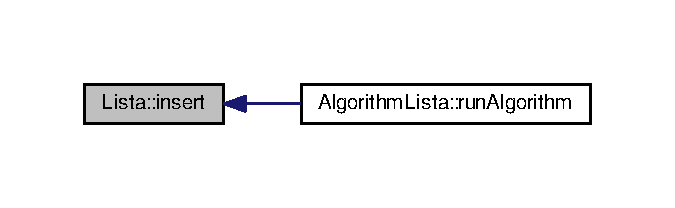
\includegraphics[width=324pt]{class_lista_acec8ac807da644d8250c3c6043a208e1_icgraph}
\end{center}
\end{figure}


\hypertarget{class_lista_aa30ec43a5b51a0e37ffe8f098c5dcaa8}{\index{Lista@{Lista}!remove@{remove}}
\index{remove@{remove}!Lista@{Lista}}
\subsubsection[{remove}]{\setlength{\rightskip}{0pt plus 5cm}void Lista\-::remove (
\begin{DoxyParamCaption}
\item[{int}]{\-\_\-f}
\end{DoxyParamCaption}
)}}\label{class_lista_aa30ec43a5b51a0e37ffe8f098c5dcaa8}

\begin{DoxyParams}[1]{Parametry}
\mbox{\tt in}  & {\em \-\_\-f} & -\/ indeks elementu do usuniecia. \\
\hline
\end{DoxyParams}


Definicja w linii 19 pliku lista.\-cpp.



\subsection{Dokumentacja atrybutów składowych}
\hypertarget{class_lista_aeba20505030183d334971bd44c3c8b95}{\index{Lista@{Lista}!head@{head}}
\index{head@{head}!Lista@{Lista}}
\subsubsection[{head}]{\setlength{\rightskip}{0pt plus 5cm}{\bf Komorka}$\ast$ Lista\-::head\hspace{0.3cm}{\ttfamily [private]}}}\label{class_lista_aeba20505030183d334971bd44c3c8b95}


Definicja w linii 38 pliku lista.\-hh.

\hypertarget{class_lista_a7d42e5f99e945d97c29d6f764f71f4e7}{\index{Lista@{Lista}!tail@{tail}}
\index{tail@{tail}!Lista@{Lista}}
\subsubsection[{tail}]{\setlength{\rightskip}{0pt plus 5cm}{\bf Komorka}$\ast$ Lista\-::tail\hspace{0.3cm}{\ttfamily [private]}}}\label{class_lista_a7d42e5f99e945d97c29d6f764f71f4e7}


Definicja w linii 42 pliku lista.\-hh.



Dokumentacja dla tej klasy została wygenerowana z plików\-:\begin{DoxyCompactItemize}
\item 
\hyperlink{lista_8hh}{lista.\-hh}\item 
\hyperlink{lista_8cpp}{lista.\-cpp}\end{DoxyCompactItemize}

\hypertarget{class_mieszajaca}{\section{Dokumentacja klasy Mieszajaca}
\label{class_mieszajaca}\index{Mieszajaca@{Mieszajaca}}
}


Klasa \hyperlink{class_mieszajaca}{Mieszajaca}. Obiekt tego typu reprezentuje pojedyncza strukture danych typu tablica mieszajaca wraz z operacjami mozliwymi do wykonania na tej strukturze.  




{\ttfamily \#include $<$mieszajaca.\-hh$>$}



Diagram współpracy dla Mieszajaca\-:
\nopagebreak
\begin{figure}[H]
\begin{center}
\leavevmode
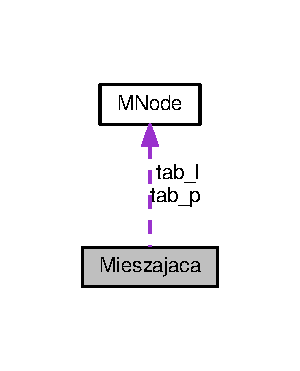
\includegraphics[width=144pt]{class_mieszajaca__coll__graph}
\end{center}
\end{figure}
\subsection*{Metody publiczne}
\begin{DoxyCompactItemize}
\item 
\hyperlink{class_mieszajaca_ab500c9ba068fbe15f9aa05d83df500ed}{Mieszajaca} ()
\begin{DoxyCompactList}\small\item\em Konstruktor obiektu \hyperlink{class_mieszajaca}{Mieszajaca}. \end{DoxyCompactList}\item 
\hyperlink{class_mieszajaca_a057f62fac3404b4748b4b38dbfc25cc2}{Mieszajaca} (long \-\_\-size)
\begin{DoxyCompactList}\small\item\em Konstruktor parametryczny obiektu mieszajaca. \end{DoxyCompactList}\item 
\hyperlink{class_mieszajaca_a66a712ce4807c9330ae36f6561101a57}{$\sim$\-Mieszajaca} ()
\begin{DoxyCompactList}\small\item\em Destruktor obiektu \hyperlink{class_mieszajaca}{Mieszajaca}. \end{DoxyCompactList}\item 
int \& \hyperlink{class_mieszajaca_ad2a90e2facd4df39cd1efe8a75ce60a4}{operator\mbox{[}$\,$\mbox{]}} (const char $\ast$key)
\begin{DoxyCompactList}\small\item\em Przeladowanie operatora nawiasu kwadratowego. Sluzy do wpisywania klucza oraz wartosci. \end{DoxyCompactList}\end{DoxyCompactItemize}
\subsection*{Metody chronione}
\begin{DoxyCompactItemize}
\item 
unsigned \hyperlink{class_mieszajaca_a4508ea747690242d296d5095ccd6e2ec}{sax\-\_\-hash} (const char $\ast$key) const 
\begin{DoxyCompactList}\small\item\em Funkcja haszująca Shift-\/\-Add-\/\-X\-O\-R. \end{DoxyCompactList}\item 
unsigned \hyperlink{class_mieszajaca_a5367ffb855dcf48ed51deaab30896249}{fnv\-\_\-hash} (const char $\ast$key) const 
\begin{DoxyCompactList}\small\item\em Funkcja haszująca Fovler/\-Voll/\-No. \end{DoxyCompactList}\item 
\hyperlink{struct_m_node}{M\-Node} $\ast$ \hyperlink{class_mieszajaca_aade3fc649e04b21a9497d8d3b6939082}{find} (const char $\ast$key) const 
\begin{DoxyCompactList}\small\item\em Metoda wyszukiwania elementu o podanym kluczu. \end{DoxyCompactList}\item 
void \hyperlink{class_mieszajaca_a6c58c6edcfac89082e7d49538c8e5c74}{insert} (const char $\ast$key, int value)
\begin{DoxyCompactList}\small\item\em Metoda wstawiania nowej pary klucz-\/wartosc. \end{DoxyCompactList}\end{DoxyCompactItemize}
\subsection*{Atrybuty prywatne}
\begin{DoxyCompactItemize}
\item 
\hyperlink{struct_m_node}{M\-Node} $\ast$$\ast$ \hyperlink{class_mieszajaca_adb0f4884ed63b184cf0bd63e757490cd}{tab\-\_\-l}
\begin{DoxyCompactList}\small\item\em Wskaznik na lewa tablice elementow. \end{DoxyCompactList}\item 
\hyperlink{struct_m_node}{M\-Node} $\ast$$\ast$ \hyperlink{class_mieszajaca_a37e86d776d7eeef64b36f04e91b44a4c}{tab\-\_\-p}
\begin{DoxyCompactList}\small\item\em Wskaznik na lewa tablice elementow. \end{DoxyCompactList}\item 
long \hyperlink{class_mieszajaca_a6521d97bf16d4fd92d147aafd2a56e3f}{size}
\begin{DoxyCompactList}\small\item\em Rozmiar tablic. \end{DoxyCompactList}\end{DoxyCompactItemize}
\subsection*{Przyjaciele}
\begin{DoxyCompactItemize}
\item 
std\-::ostream \& \hyperlink{class_mieszajaca_a6c4fd68588109e2cca8a88cee92b9a67}{operator$<$$<$} (std\-::ostream \&stream, \hyperlink{class_mieszajaca}{Mieszajaca} \&l)
\begin{DoxyCompactList}\small\item\em Przeladowanie operatora przesuniecia bitowego. Sluzy do wypisywania zawartosci tablicy mieszajacej na strumien wyjsciowy. \end{DoxyCompactList}\end{DoxyCompactItemize}


\subsection{Opis szczegółowy}


Definicja w linii 74 pliku mieszajaca.\-hh.



\subsection{Dokumentacja konstruktora i destruktora}
\hypertarget{class_mieszajaca_ab500c9ba068fbe15f9aa05d83df500ed}{\index{Mieszajaca@{Mieszajaca}!Mieszajaca@{Mieszajaca}}
\index{Mieszajaca@{Mieszajaca}!Mieszajaca@{Mieszajaca}}
\subsubsection[{Mieszajaca}]{\setlength{\rightskip}{0pt plus 5cm}Mieszajaca\-::\-Mieszajaca (
\begin{DoxyParamCaption}
{}
\end{DoxyParamCaption}
)}}\label{class_mieszajaca_ab500c9ba068fbe15f9aa05d83df500ed}


Definicja w linii 7 pliku mieszajaca.\-cpp.

\hypertarget{class_mieszajaca_a057f62fac3404b4748b4b38dbfc25cc2}{\index{Mieszajaca@{Mieszajaca}!Mieszajaca@{Mieszajaca}}
\index{Mieszajaca@{Mieszajaca}!Mieszajaca@{Mieszajaca}}
\subsubsection[{Mieszajaca}]{\setlength{\rightskip}{0pt plus 5cm}Mieszajaca\-::\-Mieszajaca (
\begin{DoxyParamCaption}
\item[{long}]{\-\_\-size}
\end{DoxyParamCaption}
)}}\label{class_mieszajaca_a057f62fac3404b4748b4b38dbfc25cc2}

\begin{DoxyParams}[1]{Parametry}
\mbox{\tt in}  & {\em \-\_\-size} & -\/ rozmiar tworzonej tablicy mieszajacej. \\
\hline
\end{DoxyParams}


Definicja w linii 19 pliku mieszajaca.\-cpp.

\hypertarget{class_mieszajaca_a66a712ce4807c9330ae36f6561101a57}{\index{Mieszajaca@{Mieszajaca}!$\sim$\-Mieszajaca@{$\sim$\-Mieszajaca}}
\index{$\sim$\-Mieszajaca@{$\sim$\-Mieszajaca}!Mieszajaca@{Mieszajaca}}
\subsubsection[{$\sim$\-Mieszajaca}]{\setlength{\rightskip}{0pt plus 5cm}Mieszajaca\-::$\sim$\-Mieszajaca (
\begin{DoxyParamCaption}
{}
\end{DoxyParamCaption}
)}}\label{class_mieszajaca_a66a712ce4807c9330ae36f6561101a57}


Definicja w linii 31 pliku mieszajaca.\-cpp.



\subsection{Dokumentacja funkcji składowych}
\hypertarget{class_mieszajaca_aade3fc649e04b21a9497d8d3b6939082}{\index{Mieszajaca@{Mieszajaca}!find@{find}}
\index{find@{find}!Mieszajaca@{Mieszajaca}}
\subsubsection[{find}]{\setlength{\rightskip}{0pt plus 5cm}{\bf M\-Node} $\ast$ Mieszajaca\-::find (
\begin{DoxyParamCaption}
\item[{const char $\ast$}]{key}
\end{DoxyParamCaption}
) const\hspace{0.3cm}{\ttfamily [protected]}}}\label{class_mieszajaca_aade3fc649e04b21a9497d8d3b6939082}

\begin{DoxyParams}[1]{Parametry}
\mbox{\tt in}  & {\em key} & -\/ wskaznik na wyszukiwany klucz. \\
\hline
\end{DoxyParams}
\begin{DoxyReturn}{Zwraca}
wskaznik na szukana pare klucz-\/wartosc, nullprt gdy nie znalezniono klucza. 
\end{DoxyReturn}


Definicja w linii 90 pliku mieszajaca.\-cpp.



Oto graf wywołań dla tej funkcji\-:
\nopagebreak
\begin{figure}[H]
\begin{center}
\leavevmode
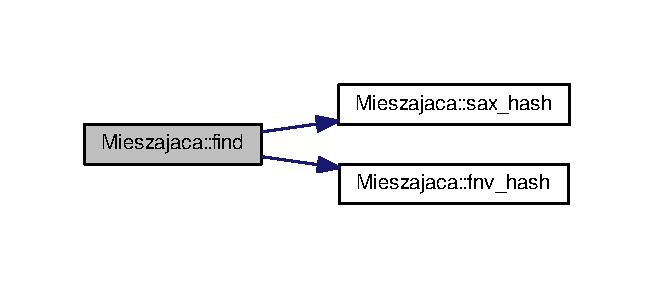
\includegraphics[width=314pt]{class_mieszajaca_aade3fc649e04b21a9497d8d3b6939082_cgraph}
\end{center}
\end{figure}




Oto graf wywoływań tej funkcji\-:
\nopagebreak
\begin{figure}[H]
\begin{center}
\leavevmode
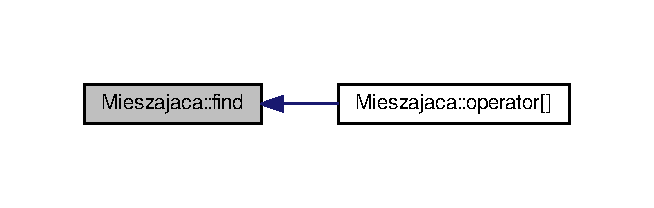
\includegraphics[width=314pt]{class_mieszajaca_aade3fc649e04b21a9497d8d3b6939082_icgraph}
\end{center}
\end{figure}


\hypertarget{class_mieszajaca_a5367ffb855dcf48ed51deaab30896249}{\index{Mieszajaca@{Mieszajaca}!fnv\-\_\-hash@{fnv\-\_\-hash}}
\index{fnv\-\_\-hash@{fnv\-\_\-hash}!Mieszajaca@{Mieszajaca}}
\subsubsection[{fnv\-\_\-hash}]{\setlength{\rightskip}{0pt plus 5cm}unsigned Mieszajaca\-::fnv\-\_\-hash (
\begin{DoxyParamCaption}
\item[{const char $\ast$}]{key}
\end{DoxyParamCaption}
) const\hspace{0.3cm}{\ttfamily [protected]}}}\label{class_mieszajaca_a5367ffb855dcf48ed51deaab30896249}

\begin{DoxyParams}[1]{Parametry}
\mbox{\tt in}  & {\em key} & -\/ wskaznik na wyszukiwany klucz. \\
\hline
\end{DoxyParams}
\begin{DoxyReturn}{Zwraca}
indeks. 
\end{DoxyReturn}


Definicja w linii 55 pliku mieszajaca.\-cpp.



Oto graf wywoływań tej funkcji\-:
\nopagebreak
\begin{figure}[H]
\begin{center}
\leavevmode
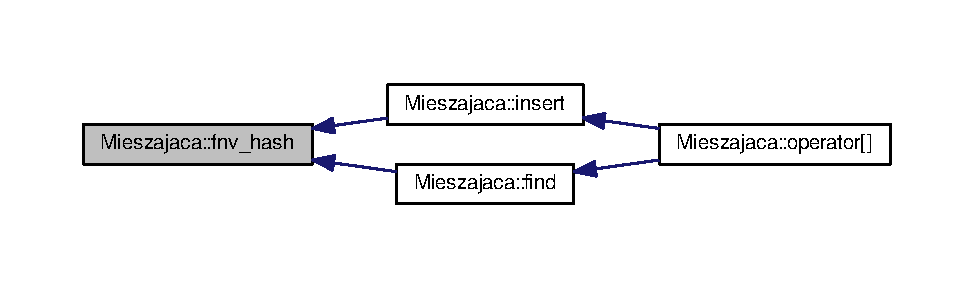
\includegraphics[width=350pt]{class_mieszajaca_a5367ffb855dcf48ed51deaab30896249_icgraph}
\end{center}
\end{figure}


\hypertarget{class_mieszajaca_a6c58c6edcfac89082e7d49538c8e5c74}{\index{Mieszajaca@{Mieszajaca}!insert@{insert}}
\index{insert@{insert}!Mieszajaca@{Mieszajaca}}
\subsubsection[{insert}]{\setlength{\rightskip}{0pt plus 5cm}void Mieszajaca\-::insert (
\begin{DoxyParamCaption}
\item[{const char $\ast$}]{key, }
\item[{int}]{value}
\end{DoxyParamCaption}
)\hspace{0.3cm}{\ttfamily [protected]}}}\label{class_mieszajaca_a6c58c6edcfac89082e7d49538c8e5c74}

\begin{DoxyParams}[1]{Parametry}
\mbox{\tt in}  & {\em key} & -\/ wskaznik na klucz. \\
\hline
\mbox{\tt in}  & {\em value} & -\/ wartosc klucza. \\
\hline
\end{DoxyParams}


Definicja w linii 71 pliku mieszajaca.\-cpp.



Oto graf wywołań dla tej funkcji\-:
\nopagebreak
\begin{figure}[H]
\begin{center}
\leavevmode
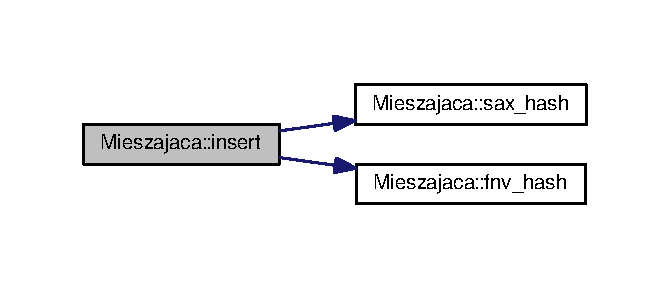
\includegraphics[width=322pt]{class_mieszajaca_a6c58c6edcfac89082e7d49538c8e5c74_cgraph}
\end{center}
\end{figure}




Oto graf wywoływań tej funkcji\-:
\nopagebreak
\begin{figure}[H]
\begin{center}
\leavevmode
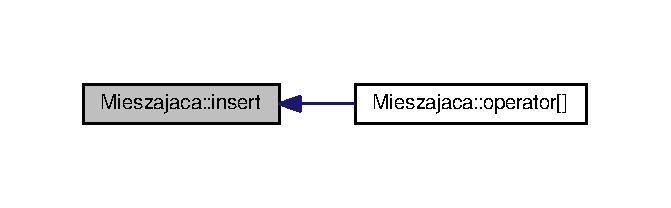
\includegraphics[width=322pt]{class_mieszajaca_a6c58c6edcfac89082e7d49538c8e5c74_icgraph}
\end{center}
\end{figure}


\hypertarget{class_mieszajaca_ad2a90e2facd4df39cd1efe8a75ce60a4}{\index{Mieszajaca@{Mieszajaca}!operator\mbox{[}$\,$\mbox{]}@{operator[]}}
\index{operator\mbox{[}$\,$\mbox{]}@{operator[]}!Mieszajaca@{Mieszajaca}}
\subsubsection[{operator[]}]{\setlength{\rightskip}{0pt plus 5cm}int \& Mieszajaca\-::operator\mbox{[}$\,$\mbox{]} (
\begin{DoxyParamCaption}
\item[{const char $\ast$}]{key}
\end{DoxyParamCaption}
)}}\label{class_mieszajaca_ad2a90e2facd4df39cd1efe8a75ce60a4}

\begin{DoxyParams}[1]{Parametry}
\mbox{\tt in}  & {\em key} & -\/ wskaznik na klucz. \\
\hline
\end{DoxyParams}
\begin{DoxyReturn}{Zwraca}
wartosc klucza. 
\end{DoxyReturn}


Definicja w linii 108 pliku mieszajaca.\-cpp.



Oto graf wywołań dla tej funkcji\-:
\nopagebreak
\begin{figure}[H]
\begin{center}
\leavevmode
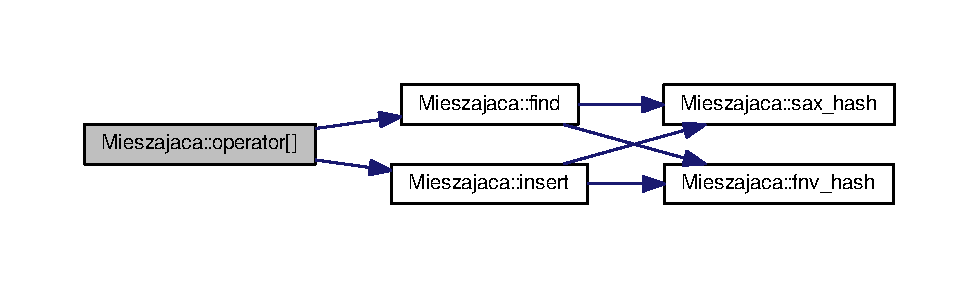
\includegraphics[width=350pt]{class_mieszajaca_ad2a90e2facd4df39cd1efe8a75ce60a4_cgraph}
\end{center}
\end{figure}


\hypertarget{class_mieszajaca_a4508ea747690242d296d5095ccd6e2ec}{\index{Mieszajaca@{Mieszajaca}!sax\-\_\-hash@{sax\-\_\-hash}}
\index{sax\-\_\-hash@{sax\-\_\-hash}!Mieszajaca@{Mieszajaca}}
\subsubsection[{sax\-\_\-hash}]{\setlength{\rightskip}{0pt plus 5cm}unsigned Mieszajaca\-::sax\-\_\-hash (
\begin{DoxyParamCaption}
\item[{const char $\ast$}]{key}
\end{DoxyParamCaption}
) const\hspace{0.3cm}{\ttfamily [protected]}}}\label{class_mieszajaca_a4508ea747690242d296d5095ccd6e2ec}

\begin{DoxyParams}[1]{Parametry}
\mbox{\tt in}  & {\em key} & -\/ wskaznik na wyszukiwany klucz. \\
\hline
\end{DoxyParams}
\begin{DoxyReturn}{Zwraca}
indeks. 
\end{DoxyReturn}


Definicja w linii 38 pliku mieszajaca.\-cpp.



Oto graf wywoływań tej funkcji\-:
\nopagebreak
\begin{figure}[H]
\begin{center}
\leavevmode
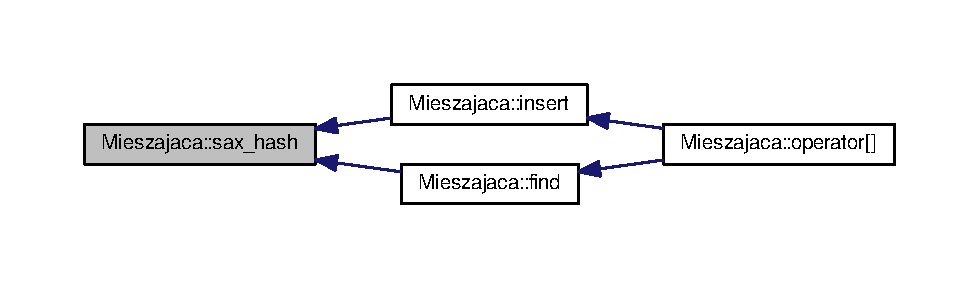
\includegraphics[width=350pt]{class_mieszajaca_a4508ea747690242d296d5095ccd6e2ec_icgraph}
\end{center}
\end{figure}




\subsection{Dokumentacja przyjaciół i funkcji związanych}
\hypertarget{class_mieszajaca_a6c4fd68588109e2cca8a88cee92b9a67}{\index{Mieszajaca@{Mieszajaca}!operator$<$$<$@{operator$<$$<$}}
\index{operator$<$$<$@{operator$<$$<$}!Mieszajaca@{Mieszajaca}}
\subsubsection[{operator$<$$<$}]{\setlength{\rightskip}{0pt plus 5cm}std\-::ostream\& operator$<$$<$ (
\begin{DoxyParamCaption}
\item[{std\-::ostream \&}]{stream, }
\item[{{\bf Mieszajaca} \&}]{l}
\end{DoxyParamCaption}
)\hspace{0.3cm}{\ttfamily [friend]}}}\label{class_mieszajaca_a6c4fd68588109e2cca8a88cee92b9a67}

\begin{DoxyParams}[1]{Parametry}
\mbox{\tt in}  & {\em stream} & -\/ referencja do strumienia wyjsciowego. \\
\hline
\mbox{\tt in}  & {\em l} & -\/ referencja do tablicy. \\
\hline
\end{DoxyParams}
\begin{DoxyReturn}{Zwraca}
strumien wyjsciowy. 
\end{DoxyReturn}


Definicja w linii 147 pliku mieszajaca.\-hh.



\subsection{Dokumentacja atrybutów składowych}
\hypertarget{class_mieszajaca_a6521d97bf16d4fd92d147aafd2a56e3f}{\index{Mieszajaca@{Mieszajaca}!size@{size}}
\index{size@{size}!Mieszajaca@{Mieszajaca}}
\subsubsection[{size}]{\setlength{\rightskip}{0pt plus 5cm}long Mieszajaca\-::size\hspace{0.3cm}{\ttfamily [private]}}}\label{class_mieszajaca_a6521d97bf16d4fd92d147aafd2a56e3f}


Definicja w linii 87 pliku mieszajaca.\-hh.

\hypertarget{class_mieszajaca_adb0f4884ed63b184cf0bd63e757490cd}{\index{Mieszajaca@{Mieszajaca}!tab\-\_\-l@{tab\-\_\-l}}
\index{tab\-\_\-l@{tab\-\_\-l}!Mieszajaca@{Mieszajaca}}
\subsubsection[{tab\-\_\-l}]{\setlength{\rightskip}{0pt plus 5cm}{\bf M\-Node}$\ast$$\ast$ Mieszajaca\-::tab\-\_\-l\hspace{0.3cm}{\ttfamily [private]}}}\label{class_mieszajaca_adb0f4884ed63b184cf0bd63e757490cd}


Definicja w linii 79 pliku mieszajaca.\-hh.

\hypertarget{class_mieszajaca_a37e86d776d7eeef64b36f04e91b44a4c}{\index{Mieszajaca@{Mieszajaca}!tab\-\_\-p@{tab\-\_\-p}}
\index{tab\-\_\-p@{tab\-\_\-p}!Mieszajaca@{Mieszajaca}}
\subsubsection[{tab\-\_\-p}]{\setlength{\rightskip}{0pt plus 5cm}{\bf M\-Node}$\ast$$\ast$ Mieszajaca\-::tab\-\_\-p\hspace{0.3cm}{\ttfamily [private]}}}\label{class_mieszajaca_a37e86d776d7eeef64b36f04e91b44a4c}


Definicja w linii 83 pliku mieszajaca.\-hh.



Dokumentacja dla tej klasy została wygenerowana z plików\-:\begin{DoxyCompactItemize}
\item 
\hyperlink{mieszajaca_8hh}{mieszajaca.\-hh}\item 
\hyperlink{mieszajaca_8cpp}{mieszajaca.\-cpp}\end{DoxyCompactItemize}

\hypertarget{struct_m_node}{\section{Dokumentacja struktury M\-Node}
\label{struct_m_node}\index{M\-Node@{M\-Node}}
}


Struktura \hyperlink{struct_a_node}{A\-Node}. Obiekt tego typu reprezentuje pojedyncza komorke tablicy mieszajacej;.  




{\ttfamily \#include $<$mieszajaca.\-hh$>$}

\subsection*{Metody publiczne}
\begin{DoxyCompactItemize}
\item 
\hyperlink{struct_m_node_a4f5e9c524bf97b5694d8f008e9436996}{M\-Node} ()
\item 
\hyperlink{struct_m_node_a579e99923a2f7cdacc468d2df179f9c3}{M\-Node} (const char $\ast$k)
\begin{DoxyCompactList}\small\item\em Konstruktor paramteryczny struktury \hyperlink{struct_m_node}{M\-Node}. \end{DoxyCompactList}\item 
\hyperlink{struct_m_node_a9fc5ae595ed230ab6af613daf0363303}{M\-Node} (const \hyperlink{struct_m_node}{M\-Node} \&s)
\begin{DoxyCompactList}\small\item\em Konstruktor paramteryczny struktury \hyperlink{struct_m_node}{M\-Node}. \end{DoxyCompactList}\item 
\hyperlink{struct_m_node_aa96f44f28eee1e25a9a267baaa61813d}{$\sim$\-M\-Node} ()
\begin{DoxyCompactList}\small\item\em Destruktor struktury node. \end{DoxyCompactList}\end{DoxyCompactItemize}
\subsection*{Atrybuty publiczne}
\begin{DoxyCompactItemize}
\item 
char $\ast$ \hyperlink{struct_m_node_a34eaceeae213bc93c9f18b752801a1f0}{key}
\begin{DoxyCompactList}\small\item\em Wskaznik na klucz. \end{DoxyCompactList}\item 
int \hyperlink{struct_m_node_a9ba04f597c758c10b9f2309322fe4c8d}{val}
\begin{DoxyCompactList}\small\item\em Wartosc klucza. \end{DoxyCompactList}\end{DoxyCompactItemize}
\subsection*{Metody prywatne}
\begin{DoxyCompactItemize}
\item 
\hyperlink{struct_m_node}{M\-Node} \& \hyperlink{struct_m_node_a6b2f4245f982546c8437f599bcf410b1}{operator=} (const \hyperlink{struct_m_node}{M\-Node} \&)
\begin{DoxyCompactList}\small\item\em Przeladowanie operatora przypisania. Zabezpieczenie przed automatycznym operatorem przypisania. \end{DoxyCompactList}\end{DoxyCompactItemize}


\subsection{Opis szczegółowy}


Definicja w linii 11 pliku mieszajaca.\-hh.



\subsection{Dokumentacja konstruktora i destruktora}
\hypertarget{struct_m_node_a4f5e9c524bf97b5694d8f008e9436996}{\index{M\-Node@{M\-Node}!M\-Node@{M\-Node}}
\index{M\-Node@{M\-Node}!MNode@{M\-Node}}
\subsubsection[{M\-Node}]{\setlength{\rightskip}{0pt plus 5cm}M\-Node\-::\-M\-Node (
\begin{DoxyParamCaption}
{}
\end{DoxyParamCaption}
)\hspace{0.3cm}{\ttfamily [inline]}}}\label{struct_m_node_a4f5e9c524bf97b5694d8f008e9436996}


Definicja w linii 21 pliku mieszajaca.\-hh.

\hypertarget{struct_m_node_a579e99923a2f7cdacc468d2df179f9c3}{\index{M\-Node@{M\-Node}!M\-Node@{M\-Node}}
\index{M\-Node@{M\-Node}!MNode@{M\-Node}}
\subsubsection[{M\-Node}]{\setlength{\rightskip}{0pt plus 5cm}M\-Node\-::\-M\-Node (
\begin{DoxyParamCaption}
\item[{const char $\ast$}]{k}
\end{DoxyParamCaption}
)\hspace{0.3cm}{\ttfamily [inline]}}}\label{struct_m_node_a579e99923a2f7cdacc468d2df179f9c3}

\begin{DoxyParams}[1]{Parametry}
\mbox{\tt in}  & {\em k} & -\/ wskaznik na klucz. \\
\hline
\end{DoxyParams}


Definicja w linii 30 pliku mieszajaca.\-hh.

\hypertarget{struct_m_node_a9fc5ae595ed230ab6af613daf0363303}{\index{M\-Node@{M\-Node}!M\-Node@{M\-Node}}
\index{M\-Node@{M\-Node}!MNode@{M\-Node}}
\subsubsection[{M\-Node}]{\setlength{\rightskip}{0pt plus 5cm}M\-Node\-::\-M\-Node (
\begin{DoxyParamCaption}
\item[{const {\bf M\-Node} \&}]{s}
\end{DoxyParamCaption}
)\hspace{0.3cm}{\ttfamily [inline]}}}\label{struct_m_node_a9fc5ae595ed230ab6af613daf0363303}

\begin{DoxyParams}[1]{Parametry}
\mbox{\tt in}  & {\em s} & -\/ referencja do pary klucz-\/wartosc. \\
\hline
\end{DoxyParams}


Definicja w linii 39 pliku mieszajaca.\-hh.

\hypertarget{struct_m_node_aa96f44f28eee1e25a9a267baaa61813d}{\index{M\-Node@{M\-Node}!$\sim$\-M\-Node@{$\sim$\-M\-Node}}
\index{$\sim$\-M\-Node@{$\sim$\-M\-Node}!MNode@{M\-Node}}
\subsubsection[{$\sim$\-M\-Node}]{\setlength{\rightskip}{0pt plus 5cm}M\-Node\-::$\sim$\-M\-Node (
\begin{DoxyParamCaption}
{}
\end{DoxyParamCaption}
)\hspace{0.3cm}{\ttfamily [inline]}}}\label{struct_m_node_aa96f44f28eee1e25a9a267baaa61813d}


Definicja w linii 54 pliku mieszajaca.\-hh.



\subsection{Dokumentacja funkcji składowych}
\hypertarget{struct_m_node_a6b2f4245f982546c8437f599bcf410b1}{\index{M\-Node@{M\-Node}!operator=@{operator=}}
\index{operator=@{operator=}!MNode@{M\-Node}}
\subsubsection[{operator=}]{\setlength{\rightskip}{0pt plus 5cm}{\bf M\-Node}\& M\-Node\-::operator= (
\begin{DoxyParamCaption}
\item[{const {\bf M\-Node} \&}]{}
\end{DoxyParamCaption}
)\hspace{0.3cm}{\ttfamily [private]}}}\label{struct_m_node_a6b2f4245f982546c8437f599bcf410b1}


\subsection{Dokumentacja atrybutów składowych}
\hypertarget{struct_m_node_a34eaceeae213bc93c9f18b752801a1f0}{\index{M\-Node@{M\-Node}!key@{key}}
\index{key@{key}!MNode@{M\-Node}}
\subsubsection[{key}]{\setlength{\rightskip}{0pt plus 5cm}char$\ast$ M\-Node\-::key}}\label{struct_m_node_a34eaceeae213bc93c9f18b752801a1f0}


Definicja w linii 15 pliku mieszajaca.\-hh.

\hypertarget{struct_m_node_a9ba04f597c758c10b9f2309322fe4c8d}{\index{M\-Node@{M\-Node}!val@{val}}
\index{val@{val}!MNode@{M\-Node}}
\subsubsection[{val}]{\setlength{\rightskip}{0pt plus 5cm}int M\-Node\-::val}}\label{struct_m_node_a9ba04f597c758c10b9f2309322fe4c8d}


Definicja w linii 19 pliku mieszajaca.\-hh.



Dokumentacja dla tej struktury została wygenerowana z pliku\-:\begin{DoxyCompactItemize}
\item 
\hyperlink{mieszajaca_8hh}{mieszajaca.\-hh}\end{DoxyCompactItemize}

\hypertarget{class_stos}{\section{Dokumentacja klasy Stos}
\label{class_stos}\index{Stos@{Stos}}
}


Klasa \hyperlink{class_stos}{Stos} modelujaca strukture danych typu stos. Obiekt tego typu reprezentuje strukture danych typu stos wraz z operacjami mozliwymi do wykonania na tej strukturze.  




{\ttfamily \#include $<$stos.\-hh$>$}

\subsection*{Metody publiczne}
\begin{DoxyCompactItemize}
\item 
\hyperlink{class_stos_a1de3b50386d5dfb56ddece17d0ea2389}{Stos} ()
\begin{DoxyCompactList}\small\item\em Konstruktor obiektu \hyperlink{class_stos}{Stos}. \end{DoxyCompactList}\item 
\hyperlink{class_stos_a6606affc11eed2b059b8caf287ffca25}{Stos} (long \-\_\-size)
\begin{DoxyCompactList}\small\item\em Konstruktor parametryczny obiektu \hyperlink{class_stos}{Stos}. \end{DoxyCompactList}\item 
\hyperlink{class_stos_af9a198e2540e18adcc0b5259105fd78e}{$\sim$\-Stos} ()
\begin{DoxyCompactList}\small\item\em Destruktor obiektu \hyperlink{class_stos}{Stos}. \end{DoxyCompactList}\item 
void \hyperlink{class_stos_afd5802e405946328cccca3eed676b493}{push} (int \-\_\-elem)
\begin{DoxyCompactList}\small\item\em Metoda dodawnia elementu. Metoda sluzy do dodawania elementu do stosu. \end{DoxyCompactList}\item 
int \hyperlink{class_stos_aabb14b8a389c55da6e2b50fbb179ed56}{pop} ()
\begin{DoxyCompactList}\small\item\em Metoda usuwania elementu. Metoda sluzy do usuwania elementu ze stosu. \end{DoxyCompactList}\end{DoxyCompactItemize}
\subsection*{Metody prywatne}
\begin{DoxyCompactItemize}
\item 
void \hyperlink{class_stos_aaf6e4717d1983c5351c9f5e9797368d3}{increase} ()
\begin{DoxyCompactList}\small\item\em Metoda powiekszania stosu. Metoda ta dodaje do stosu 8 kolejnych wolnych pol. \end{DoxyCompactList}\item 
int \hyperlink{class_stos_a1054dda0231b2516b6a04298801c0b27}{decrease} ()
\begin{DoxyCompactList}\small\item\em Metoda pomniejszania stosu. Metoda ta odejmuje od stosu jedno pole. \end{DoxyCompactList}\end{DoxyCompactItemize}
\subsection*{Atrybuty prywatne}
\begin{DoxyCompactItemize}
\item 
int $\ast$ \hyperlink{class_stos_abcb666dd5a69fe50228595dc8ac4160a}{tab}
\begin{DoxyCompactList}\small\item\em Wskaznik na tablice elementow stosu. \end{DoxyCompactList}\item 
long \hyperlink{class_stos_a07ba18a24f8f0dbd9144406d15bcd342}{size}
\begin{DoxyCompactList}\small\item\em Rozmiar stosu. \end{DoxyCompactList}\item 
long \hyperlink{class_stos_ae0623cdf9b6725e38da86b74972d61ba}{last}
\begin{DoxyCompactList}\small\item\em Indeks ostatniego wolnego pola. \end{DoxyCompactList}\end{DoxyCompactItemize}


\subsection{Opis szczegółowy}


Definicja w linii 9 pliku stos.\-hh.



\subsection{Dokumentacja konstruktora i destruktora}
\hypertarget{class_stos_a1de3b50386d5dfb56ddece17d0ea2389}{\index{Stos@{Stos}!Stos@{Stos}}
\index{Stos@{Stos}!Stos@{Stos}}
\subsubsection[{Stos}]{\setlength{\rightskip}{0pt plus 5cm}Stos\-::\-Stos (
\begin{DoxyParamCaption}
{}
\end{DoxyParamCaption}
)}}\label{class_stos_a1de3b50386d5dfb56ddece17d0ea2389}


Definicja w linii 6 pliku stos.\-cpp.

\hypertarget{class_stos_a6606affc11eed2b059b8caf287ffca25}{\index{Stos@{Stos}!Stos@{Stos}}
\index{Stos@{Stos}!Stos@{Stos}}
\subsubsection[{Stos}]{\setlength{\rightskip}{0pt plus 5cm}Stos\-::\-Stos (
\begin{DoxyParamCaption}
\item[{long}]{\-\_\-size}
\end{DoxyParamCaption}
)}}\label{class_stos_a6606affc11eed2b059b8caf287ffca25}

\begin{DoxyParams}[1]{Parametry}
\mbox{\tt in}  & {\em \-\_\-size} & -\/ rozmiar tworzonego stosu. \\
\hline
\end{DoxyParams}


Definicja w linii 17 pliku stos.\-cpp.

\hypertarget{class_stos_af9a198e2540e18adcc0b5259105fd78e}{\index{Stos@{Stos}!$\sim$\-Stos@{$\sim$\-Stos}}
\index{$\sim$\-Stos@{$\sim$\-Stos}!Stos@{Stos}}
\subsubsection[{$\sim$\-Stos}]{\setlength{\rightskip}{0pt plus 5cm}Stos\-::$\sim$\-Stos (
\begin{DoxyParamCaption}
{}
\end{DoxyParamCaption}
)}}\label{class_stos_af9a198e2540e18adcc0b5259105fd78e}


Definicja w linii 28 pliku stos.\-cpp.



\subsection{Dokumentacja funkcji składowych}
\hypertarget{class_stos_a1054dda0231b2516b6a04298801c0b27}{\index{Stos@{Stos}!decrease@{decrease}}
\index{decrease@{decrease}!Stos@{Stos}}
\subsubsection[{decrease}]{\setlength{\rightskip}{0pt plus 5cm}int Stos\-::decrease (
\begin{DoxyParamCaption}
{}
\end{DoxyParamCaption}
)\hspace{0.3cm}{\ttfamily [private]}}}\label{class_stos_a1054dda0231b2516b6a04298801c0b27}


Definicja w linii 63 pliku stos.\-cpp.



Oto graf wywoływań tej funkcji\-:\nopagebreak
\begin{figure}[H]
\begin{center}
\leavevmode
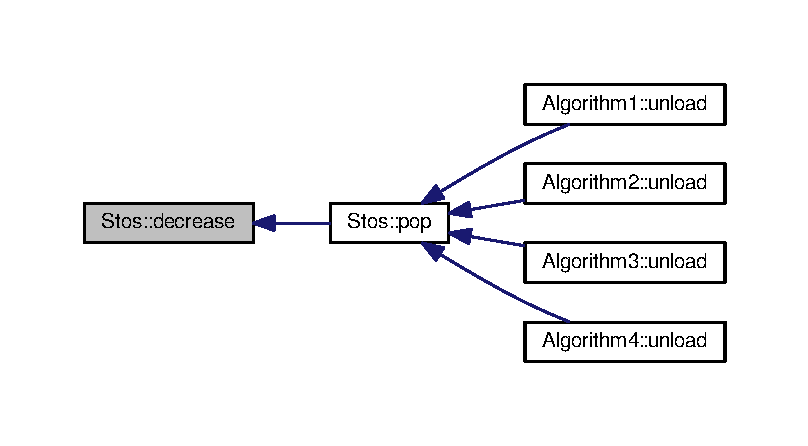
\includegraphics[width=256pt]{class_stos_a1054dda0231b2516b6a04298801c0b27_icgraph}
\end{center}
\end{figure}


\hypertarget{class_stos_aaf6e4717d1983c5351c9f5e9797368d3}{\index{Stos@{Stos}!increase@{increase}}
\index{increase@{increase}!Stos@{Stos}}
\subsubsection[{increase}]{\setlength{\rightskip}{0pt plus 5cm}void Stos\-::increase (
\begin{DoxyParamCaption}
{}
\end{DoxyParamCaption}
)\hspace{0.3cm}{\ttfamily [private]}}}\label{class_stos_aaf6e4717d1983c5351c9f5e9797368d3}


Definicja w linii 51 pliku stos.\-cpp.



Oto graf wywoływań tej funkcji\-:\nopagebreak
\begin{figure}[H]
\begin{center}
\leavevmode
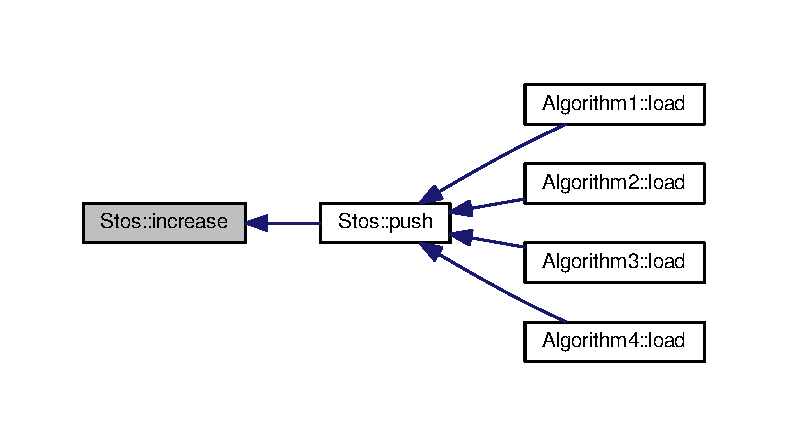
\includegraphics[width=350pt]{class_stos_aaf6e4717d1983c5351c9f5e9797368d3_icgraph}
\end{center}
\end{figure}


\hypertarget{class_stos_aabb14b8a389c55da6e2b50fbb179ed56}{\index{Stos@{Stos}!pop@{pop}}
\index{pop@{pop}!Stos@{Stos}}
\subsubsection[{pop}]{\setlength{\rightskip}{0pt plus 5cm}int Stos\-::pop (
\begin{DoxyParamCaption}
{}
\end{DoxyParamCaption}
)}}\label{class_stos_aabb14b8a389c55da6e2b50fbb179ed56}
\begin{DoxyReturn}{Zwraca}
-\/ usuwany element. 
\end{DoxyReturn}


Definicja w linii 43 pliku stos.\-cpp.



Oto graf wywołań dla tej funkcji\-:\nopagebreak
\begin{figure}[H]
\begin{center}
\leavevmode
\includegraphics[width=256pt]{class_stos_aabb14b8a389c55da6e2b50fbb179ed56_cgraph}
\end{center}
\end{figure}


\hypertarget{class_stos_afd5802e405946328cccca3eed676b493}{\index{Stos@{Stos}!push@{push}}
\index{push@{push}!Stos@{Stos}}
\subsubsection[{push}]{\setlength{\rightskip}{0pt plus 5cm}void Stos\-::push (
\begin{DoxyParamCaption}
\item[{int}]{\-\_\-elem}
\end{DoxyParamCaption}
)}}\label{class_stos_afd5802e405946328cccca3eed676b493}

\begin{DoxyParams}[1]{Parametry}
\mbox{\tt in}  & {\em \-\_\-elem} & -\/ dodawany element. \\
\hline
\end{DoxyParams}


Definicja w linii 34 pliku stos.\-cpp.



Oto graf wywołań dla tej funkcji\-:\nopagebreak
\begin{figure}[H]
\begin{center}
\leavevmode
\includegraphics[width=256pt]{class_stos_afd5802e405946328cccca3eed676b493_cgraph}
\end{center}
\end{figure}




Oto graf wywoływań tej funkcji\-:\nopagebreak
\begin{figure}[H]
\begin{center}
\leavevmode
\includegraphics[width=316pt]{class_stos_afd5802e405946328cccca3eed676b493_icgraph}
\end{center}
\end{figure}




\subsection{Dokumentacja atrybutów składowych}
\hypertarget{class_stos_ae0623cdf9b6725e38da86b74972d61ba}{\index{Stos@{Stos}!last@{last}}
\index{last@{last}!Stos@{Stos}}
\subsubsection[{last}]{\setlength{\rightskip}{0pt plus 5cm}long Stos\-::last\hspace{0.3cm}{\ttfamily [private]}}}\label{class_stos_ae0623cdf9b6725e38da86b74972d61ba}


Definicja w linii 22 pliku stos.\-hh.

\hypertarget{class_stos_a07ba18a24f8f0dbd9144406d15bcd342}{\index{Stos@{Stos}!size@{size}}
\index{size@{size}!Stos@{Stos}}
\subsubsection[{size}]{\setlength{\rightskip}{0pt plus 5cm}long Stos\-::size\hspace{0.3cm}{\ttfamily [private]}}}\label{class_stos_a07ba18a24f8f0dbd9144406d15bcd342}


Definicja w linii 18 pliku stos.\-hh.

\hypertarget{class_stos_abcb666dd5a69fe50228595dc8ac4160a}{\index{Stos@{Stos}!tab@{tab}}
\index{tab@{tab}!Stos@{Stos}}
\subsubsection[{tab}]{\setlength{\rightskip}{0pt plus 5cm}int$\ast$ Stos\-::tab\hspace{0.3cm}{\ttfamily [private]}}}\label{class_stos_abcb666dd5a69fe50228595dc8ac4160a}


Definicja w linii 14 pliku stos.\-hh.



Dokumentacja dla tej klasy została wygenerowana z plików\-:\begin{DoxyCompactItemize}
\item 
\hyperlink{stos_8hh}{stos.\-hh}\item 
\hyperlink{stos_8cpp}{stos.\-cpp}\end{DoxyCompactItemize}

\hypertarget{class_tab_lista}{\section{Dokumentacja klasy Tab\-Lista}
\label{class_tab_lista}\index{Tab\-Lista@{Tab\-Lista}}
}


Klasa \hyperlink{class_tab_lista}{Tab\-Lista} modelujaca strukture danych typu lista. Obiekt tego typu reprezentuje strukture danych typu lista zaimplementowana na tablicy dynamicznej. Obiekt zawiera rowniez podstowe metody listy.  




{\ttfamily \#include $<$tab\-\_\-lista.\-hh$>$}

\subsection*{Metody publiczne}
\begin{DoxyCompactItemize}
\item 
\hyperlink{class_tab_lista_ad3bfa98306e98b4e5bb7ff524e72078c}{Tab\-Lista} ()
\begin{DoxyCompactList}\small\item\em Konstruktor obiektu \hyperlink{class_tab_lista}{Tab\-Lista}. \end{DoxyCompactList}\item 
\hyperlink{class_tab_lista_a95d23d52e0af187351b3fc1022ae4839}{Tab\-Lista} (long \-\_\-size)
\begin{DoxyCompactList}\small\item\em Konstruktor parametryczny obiektu \hyperlink{class_tab_lista}{Tab\-Lista}. \end{DoxyCompactList}\item 
\hyperlink{class_tab_lista_a0b4a808158b370bbc5785ceef760a273}{$\sim$\-Tab\-Lista} ()
\begin{DoxyCompactList}\small\item\em Destruktor obiektu \hyperlink{class_tab_lista}{Tab\-Lista}. \end{DoxyCompactList}\item 
void \hyperlink{class_tab_lista_a7bd3e5f62a81bfd3813ad874e8a9c059}{insert} (int \-\_\-elem)
\begin{DoxyCompactList}\small\item\em Metoda dodawnia elementu. Metoda sluzy do dodawania elementu do konca listy. \end{DoxyCompactList}\item 
int \hyperlink{class_tab_lista_aae59a3eafbbd7424a952badb26410a5e}{remove} (int \-\_\-f)
\begin{DoxyCompactList}\small\item\em Metoda usuwania elementu. Metoda sluzy do usuwania elementu o wskazanym indeksie. \end{DoxyCompactList}\end{DoxyCompactItemize}
\subsection*{Metody prywatne}
\begin{DoxyCompactItemize}
\item 
void \hyperlink{class_tab_lista_a9ae6a784d488c8b9885ccbc945225f9e}{increase} ()
\begin{DoxyCompactList}\small\item\em Metoda powiekszania listy tablicowe. Metoda ta dodaje do listy 8 kolejnych wolnych pol. \end{DoxyCompactList}\end{DoxyCompactItemize}
\subsection*{Atrybuty prywatne}
\begin{DoxyCompactItemize}
\item 
int $\ast$ \hyperlink{class_tab_lista_a06f658ed62f3db852813e90dcc5876a5}{tab}
\begin{DoxyCompactList}\small\item\em Wskaznik na tablice elementow listy. \end{DoxyCompactList}\item 
long \hyperlink{class_tab_lista_aa3c6d623be318ec8410fa447281380da}{size}
\begin{DoxyCompactList}\small\item\em Rozmiar listy. \end{DoxyCompactList}\item 
long \hyperlink{class_tab_lista_ac7413a3d41c2c2e57fa92e055fc2e5b3}{last}
\begin{DoxyCompactList}\small\item\em Wskaznik na ostatni wolny element. \end{DoxyCompactList}\end{DoxyCompactItemize}


\subsection{Opis szczegółowy}


Definicja w linii 10 pliku tab\-\_\-lista.\-hh.



\subsection{Dokumentacja konstruktora i destruktora}
\hypertarget{class_tab_lista_ad3bfa98306e98b4e5bb7ff524e72078c}{\index{Tab\-Lista@{Tab\-Lista}!Tab\-Lista@{Tab\-Lista}}
\index{Tab\-Lista@{Tab\-Lista}!TabLista@{Tab\-Lista}}
\subsubsection[{Tab\-Lista}]{\setlength{\rightskip}{0pt plus 5cm}Tab\-Lista\-::\-Tab\-Lista (
\begin{DoxyParamCaption}
{}
\end{DoxyParamCaption}
)}}\label{class_tab_lista_ad3bfa98306e98b4e5bb7ff524e72078c}


Definicja w linii 6 pliku tab\-\_\-lista.\-cpp.

\hypertarget{class_tab_lista_a95d23d52e0af187351b3fc1022ae4839}{\index{Tab\-Lista@{Tab\-Lista}!Tab\-Lista@{Tab\-Lista}}
\index{Tab\-Lista@{Tab\-Lista}!TabLista@{Tab\-Lista}}
\subsubsection[{Tab\-Lista}]{\setlength{\rightskip}{0pt plus 5cm}Tab\-Lista\-::\-Tab\-Lista (
\begin{DoxyParamCaption}
\item[{long}]{\-\_\-size}
\end{DoxyParamCaption}
)}}\label{class_tab_lista_a95d23d52e0af187351b3fc1022ae4839}


Definicja w linii 16 pliku tab\-\_\-lista.\-cpp.

\hypertarget{class_tab_lista_a0b4a808158b370bbc5785ceef760a273}{\index{Tab\-Lista@{Tab\-Lista}!$\sim$\-Tab\-Lista@{$\sim$\-Tab\-Lista}}
\index{$\sim$\-Tab\-Lista@{$\sim$\-Tab\-Lista}!TabLista@{Tab\-Lista}}
\subsubsection[{$\sim$\-Tab\-Lista}]{\setlength{\rightskip}{0pt plus 5cm}Tab\-Lista\-::$\sim$\-Tab\-Lista (
\begin{DoxyParamCaption}
{}
\end{DoxyParamCaption}
)}}\label{class_tab_lista_a0b4a808158b370bbc5785ceef760a273}


Definicja w linii 26 pliku tab\-\_\-lista.\-cpp.



\subsection{Dokumentacja funkcji składowych}
\hypertarget{class_tab_lista_a9ae6a784d488c8b9885ccbc945225f9e}{\index{Tab\-Lista@{Tab\-Lista}!increase@{increase}}
\index{increase@{increase}!TabLista@{Tab\-Lista}}
\subsubsection[{increase}]{\setlength{\rightskip}{0pt plus 5cm}void Tab\-Lista\-::increase (
\begin{DoxyParamCaption}
{}
\end{DoxyParamCaption}
)\hspace{0.3cm}{\ttfamily [private]}}}\label{class_tab_lista_a9ae6a784d488c8b9885ccbc945225f9e}


Definicja w linii 32 pliku tab\-\_\-lista.\-cpp.



Oto graf wywoływań tej funkcji\-:\nopagebreak
\begin{figure}[H]
\begin{center}
\leavevmode
\includegraphics[width=296pt]{class_tab_lista_a9ae6a784d488c8b9885ccbc945225f9e_icgraph}
\end{center}
\end{figure}


\hypertarget{class_tab_lista_a7bd3e5f62a81bfd3813ad874e8a9c059}{\index{Tab\-Lista@{Tab\-Lista}!insert@{insert}}
\index{insert@{insert}!TabLista@{Tab\-Lista}}
\subsubsection[{insert}]{\setlength{\rightskip}{0pt plus 5cm}void Tab\-Lista\-::insert (
\begin{DoxyParamCaption}
\item[{int}]{\-\_\-elem}
\end{DoxyParamCaption}
)}}\label{class_tab_lista_a7bd3e5f62a81bfd3813ad874e8a9c059}

\begin{DoxyParams}[1]{Parametry}
\mbox{\tt in}  & {\em \-\_\-elem} & -\/ dodawany element. \\
\hline
\end{DoxyParams}


Definicja w linii 44 pliku tab\-\_\-lista.\-cpp.



Oto graf wywołań dla tej funkcji\-:\nopagebreak
\begin{figure}[H]
\begin{center}
\leavevmode
\includegraphics[width=296pt]{class_tab_lista_a7bd3e5f62a81bfd3813ad874e8a9c059_cgraph}
\end{center}
\end{figure}


\hypertarget{class_tab_lista_aae59a3eafbbd7424a952badb26410a5e}{\index{Tab\-Lista@{Tab\-Lista}!remove@{remove}}
\index{remove@{remove}!TabLista@{Tab\-Lista}}
\subsubsection[{remove}]{\setlength{\rightskip}{0pt plus 5cm}int Tab\-Lista\-::remove (
\begin{DoxyParamCaption}
\item[{int}]{\-\_\-f}
\end{DoxyParamCaption}
)}}\label{class_tab_lista_aae59a3eafbbd7424a952badb26410a5e}

\begin{DoxyParams}[1]{Parametry}
\mbox{\tt in}  & {\em \-\_\-f} & -\/ indeks elementu do usuniecia. \\
\hline
\end{DoxyParams}
\begin{DoxyReturn}{Zwraca}
-\/ usuwany element. 
\end{DoxyReturn}


Definicja w linii 53 pliku tab\-\_\-lista.\-cpp.



\subsection{Dokumentacja atrybutów składowych}
\hypertarget{class_tab_lista_ac7413a3d41c2c2e57fa92e055fc2e5b3}{\index{Tab\-Lista@{Tab\-Lista}!last@{last}}
\index{last@{last}!TabLista@{Tab\-Lista}}
\subsubsection[{last}]{\setlength{\rightskip}{0pt plus 5cm}long Tab\-Lista\-::last\hspace{0.3cm}{\ttfamily [private]}}}\label{class_tab_lista_ac7413a3d41c2c2e57fa92e055fc2e5b3}


Definicja w linii 23 pliku tab\-\_\-lista.\-hh.

\hypertarget{class_tab_lista_aa3c6d623be318ec8410fa447281380da}{\index{Tab\-Lista@{Tab\-Lista}!size@{size}}
\index{size@{size}!TabLista@{Tab\-Lista}}
\subsubsection[{size}]{\setlength{\rightskip}{0pt plus 5cm}long Tab\-Lista\-::size\hspace{0.3cm}{\ttfamily [private]}}}\label{class_tab_lista_aa3c6d623be318ec8410fa447281380da}


Definicja w linii 19 pliku tab\-\_\-lista.\-hh.

\hypertarget{class_tab_lista_a06f658ed62f3db852813e90dcc5876a5}{\index{Tab\-Lista@{Tab\-Lista}!tab@{tab}}
\index{tab@{tab}!TabLista@{Tab\-Lista}}
\subsubsection[{tab}]{\setlength{\rightskip}{0pt plus 5cm}int$\ast$ Tab\-Lista\-::tab\hspace{0.3cm}{\ttfamily [private]}}}\label{class_tab_lista_a06f658ed62f3db852813e90dcc5876a5}


Definicja w linii 15 pliku tab\-\_\-lista.\-hh.



Dokumentacja dla tej klasy została wygenerowana z plików\-:\begin{DoxyCompactItemize}
\item 
\hyperlink{tab__lista_8hh}{tab\-\_\-lista.\-hh}\item 
\hyperlink{tab__lista_8cpp}{tab\-\_\-lista.\-cpp}\end{DoxyCompactItemize}

\chapter{Dokumentacja plików}
\hypertarget{algorithm1_8cpp}{\section{Dokumentacja pliku algorithm1.\-cpp}
\label{algorithm1_8cpp}\index{algorithm1.\-cpp@{algorithm1.\-cpp}}
}
{\ttfamily \#include $<$iostream$>$}\\*
{\ttfamily \#include \char`\"{}benchmark.\-hh\char`\"{}}\\*
{\ttfamily \#include \char`\"{}algorithm1.\-hh\char`\"{}}\\*
Wykres zależności załączania dla algorithm1.\-cpp\-:\nopagebreak
\begin{figure}[H]
\begin{center}
\leavevmode
\includegraphics[width=322pt]{algorithm1_8cpp__incl}
\end{center}
\end{figure}

\hypertarget{algorithm1_8hh}{\section{Dokumentacja pliku algorithm1.\-hh}
\label{algorithm1_8hh}\index{algorithm1.\-hh@{algorithm1.\-hh}}
}
Ten wykres pokazuje, które pliki bezpośrednio lub pośrednio załączają ten plik\-:\nopagebreak
\begin{figure}[H]
\begin{center}
\leavevmode
\includegraphics[width=234pt]{algorithm1_8hh__dep__incl}
\end{center}
\end{figure}
\subsection*{Komponenty}
\begin{DoxyCompactItemize}
\item 
class \hyperlink{class_algorithm1}{Algorithm1}
\begin{DoxyCompactList}\small\item\em Klasa \hyperlink{class_algorithm1}{Algorithm1} modelujaca algorytm sortowania stosu. Obiekt tego typu reprezentuje algorytm wykonujacy sortowanie szybkie na elementach stosu. Dziedziczy po klasie \hyperlink{class_benchmark}{Benchmark}. \end{DoxyCompactList}\end{DoxyCompactItemize}

\hypertarget{algorithm2_8cpp}{\section{Dokumentacja pliku algorithm2.\-cpp}
\label{algorithm2_8cpp}\index{algorithm2.\-cpp@{algorithm2.\-cpp}}
}
{\ttfamily \#include $<$iostream$>$}\\*
{\ttfamily \#include \char`\"{}stos.\-hh\char`\"{}}\\*
{\ttfamily \#include \char`\"{}benchmark.\-hh\char`\"{}}\\*
{\ttfamily \#include \char`\"{}algorithm2.\-hh\char`\"{}}\\*
Wykres zależności załączania dla algorithm2.\-cpp\-:\nopagebreak
\begin{figure}[H]
\begin{center}
\leavevmode
\includegraphics[width=350pt]{algorithm2_8cpp__incl}
\end{center}
\end{figure}

\hypertarget{algorithm2_8hh}{\section{Dokumentacja pliku algorithm2.\-hh}
\label{algorithm2_8hh}\index{algorithm2.\-hh@{algorithm2.\-hh}}
}
Ten wykres pokazuje, które pliki bezpośrednio lub pośrednio załączają ten plik\-:\nopagebreak
\begin{figure}[H]
\begin{center}
\leavevmode
\includegraphics[width=234pt]{algorithm2_8hh__dep__incl}
\end{center}
\end{figure}
\subsection*{Komponenty}
\begin{DoxyCompactItemize}
\item 
class \hyperlink{class_algorithm2}{Algorithm2}
\begin{DoxyCompactList}\small\item\em Klasa \hyperlink{class_algorithm2}{Algorithm2} modelujaca algorytm sortowania stosu. Obiekt tego typu reprezentuje algorytm wykonujacy sortowanie szybkie na elementach stosu. Dziedziczy po klasie \hyperlink{class_benchmark}{Benchmark}. \end{DoxyCompactList}\end{DoxyCompactItemize}

\hypertarget{algorithm3_8cpp}{\section{Dokumentacja pliku algorithm3.\-cpp}
\label{algorithm3_8cpp}\index{algorithm3.\-cpp@{algorithm3.\-cpp}}
}
{\ttfamily \#include $<$iostream$>$}\\*
{\ttfamily \#include \char`\"{}stos.\-hh\char`\"{}}\\*
{\ttfamily \#include \char`\"{}benchmark.\-hh\char`\"{}}\\*
{\ttfamily \#include \char`\"{}algorithm3.\-hh\char`\"{}}\\*
Wykres zależności załączania dla algorithm3.\-cpp\-:\nopagebreak
\begin{figure}[H]
\begin{center}
\leavevmode
\includegraphics[width=350pt]{algorithm3_8cpp__incl}
\end{center}
\end{figure}

\hypertarget{algorithm3_8hh}{\section{Dokumentacja pliku algorithm3.\-hh}
\label{algorithm3_8hh}\index{algorithm3.\-hh@{algorithm3.\-hh}}
}
Ten wykres pokazuje, które pliki bezpośrednio lub pośrednio załączają ten plik\-:\nopagebreak
\begin{figure}[H]
\begin{center}
\leavevmode
\includegraphics[width=234pt]{algorithm3_8hh__dep__incl}
\end{center}
\end{figure}
\subsection*{Komponenty}
\begin{DoxyCompactItemize}
\item 
class \hyperlink{class_algorithm3}{Algorithm3}
\begin{DoxyCompactList}\small\item\em Klasa \hyperlink{class_algorithm3}{Algorithm3} modelujaca algorytm sortowania stosu. Obiekt tego typu reprezentuje algorytm wykonujacy sortowanie szybkie na elementach stosu. Dziedziczy po klasie \hyperlink{class_benchmark}{Benchmark}. \end{DoxyCompactList}\end{DoxyCompactItemize}

\hypertarget{algorithm4_8cpp}{\section{Dokumentacja pliku algorithm4.\-cpp}
\label{algorithm4_8cpp}\index{algorithm4.\-cpp@{algorithm4.\-cpp}}
}
{\ttfamily \#include $<$iostream$>$}\\*
{\ttfamily \#include \char`\"{}tablicowe.\-hh\char`\"{}}\\*
{\ttfamily \#include \char`\"{}sort.\-hh\char`\"{}}\\*
{\ttfamily \#include \char`\"{}stos.\-hh\char`\"{}}\\*
{\ttfamily \#include \char`\"{}observer.\-hh\char`\"{}}\\*
{\ttfamily \#include \char`\"{}subject.\-hh\char`\"{}}\\*
{\ttfamily \#include \char`\"{}benchmark.\-hh\char`\"{}}\\*
{\ttfamily \#include \char`\"{}algorithm4.\-hh\char`\"{}}\\*
Wykres zależności załączania dla algorithm4.\-cpp\-:\nopagebreak
\begin{figure}[H]
\begin{center}
\leavevmode
\includegraphics[width=350pt]{algorithm4_8cpp__incl}
\end{center}
\end{figure}

\hypertarget{algorithm4_8hh}{\section{Dokumentacja pliku algorithm4.\-hh}
\label{algorithm4_8hh}\index{algorithm4.\-hh@{algorithm4.\-hh}}
}
Ten wykres pokazuje, które pliki bezpośrednio lub pośrednio załączają ten plik\-:
\nopagebreak
\begin{figure}[H]
\begin{center}
\leavevmode
\includegraphics[width=234pt]{algorithm4_8hh__dep__incl}
\end{center}
\end{figure}
\subsection*{Komponenty}
\begin{DoxyCompactItemize}
\item 
class \hyperlink{class_algorithm4}{Algorithm4}
\begin{DoxyCompactList}\small\item\em Klasa \hyperlink{class_algorithm4}{Algorithm4} modelujaca algorytm sortowania stosu. Obiekt tego typu reprezentuje algorytm wykonujacy sortowanie szybkie po optymalizacji na elementach stosu. Dziedziczy po klasie \hyperlink{class_benchmark}{Benchmark}. \end{DoxyCompactList}\end{DoxyCompactItemize}

\hypertarget{asocjacyjna_8cpp}{\section{Dokumentacja pliku asocjacyjna.\-cpp}
\label{asocjacyjna_8cpp}\index{asocjacyjna.\-cpp@{asocjacyjna.\-cpp}}
}
{\ttfamily \#include $<$iostream$>$}\\*
{\ttfamily \#include $<$cstring$>$}\\*
{\ttfamily \#include \char`\"{}asocjacyjna.\-hh\char`\"{}}\\*
Wykres zależności załączania dla asocjacyjna.\-cpp\-:
\nopagebreak
\begin{figure}[H]
\begin{center}
\leavevmode
\includegraphics[width=270pt]{asocjacyjna_8cpp__incl}
\end{center}
\end{figure}
\subsection*{Funkcje}
\begin{DoxyCompactItemize}
\item 
std\-::ostream \& \hyperlink{asocjacyjna_8cpp_ad2f948e16f11dff58951c8104450742e}{operator$<$$<$} (std\-::ostream \&\-\_\-stream, \hyperlink{struct_asocjacyjna}{Asocjacyjna} \&\-\_\-l)
\end{DoxyCompactItemize}


\subsection{Dokumentacja funkcji}
\hypertarget{asocjacyjna_8cpp_ad2f948e16f11dff58951c8104450742e}{\index{asocjacyjna.\-cpp@{asocjacyjna.\-cpp}!operator$<$$<$@{operator$<$$<$}}
\index{operator$<$$<$@{operator$<$$<$}!asocjacyjna.cpp@{asocjacyjna.\-cpp}}
\subsubsection[{operator$<$$<$}]{\setlength{\rightskip}{0pt plus 5cm}std\-::ostream\& operator$<$$<$ (
\begin{DoxyParamCaption}
\item[{std\-::ostream \&}]{\-\_\-stream, }
\item[{{\bf Asocjacyjna} \&}]{\-\_\-l}
\end{DoxyParamCaption}
)}}\label{asocjacyjna_8cpp_ad2f948e16f11dff58951c8104450742e}

\begin{DoxyParams}[1]{Parametry}
\mbox{\tt in}  & {\em \-\_\-stream} & -\/ referencja do strumienia wyjsciowego. \\
\hline
\mbox{\tt in}  & {\em \-\_\-l} & -\/ referencja do listy. \\
\hline
\end{DoxyParams}
\begin{DoxyReturn}{Zwraca}
strumien wyjsciowy. 
\end{DoxyReturn}


Definicja w linii 146 pliku asocjacyjna.\-cpp.


\hypertarget{asocjacyjna_8hh}{\section{Dokumentacja pliku asocjacyjna.\-hh}
\label{asocjacyjna_8hh}\index{asocjacyjna.\-hh@{asocjacyjna.\-hh}}
}
{\ttfamily \#include $<$cstring$>$}\\*
Wykres zależności załączania dla asocjacyjna.\-hh\-:\nopagebreak
\begin{figure}[H]
\begin{center}
\leavevmode
\includegraphics[width=160pt]{asocjacyjna_8hh__incl}
\end{center}
\end{figure}
Ten wykres pokazuje, które pliki bezpośrednio lub pośrednio załączają ten plik\-:\nopagebreak
\begin{figure}[H]
\begin{center}
\leavevmode
\includegraphics[width=240pt]{asocjacyjna_8hh__dep__incl}
\end{center}
\end{figure}
\subsection*{Komponenty}
\begin{DoxyCompactItemize}
\item 
struct \hyperlink{struct_a_node}{A\-Node}
\begin{DoxyCompactList}\small\item\em Struktura \hyperlink{struct_a_node}{A\-Node}. Obiekt tego typu reprezentuje pojedyncza komorke wraz ze wskaznikiem na nastepna komorke listy. \end{DoxyCompactList}\item 
struct \hyperlink{struct_asocjacyjna}{Asocjacyjna}
\begin{DoxyCompactList}\small\item\em Klasa \hyperlink{struct_asocjacyjna}{Asocjacyjna}. Obiekt tego typu reprezentuje strukture danych typu lista asocjacyjna wraz z operacjami mozliwymi do wykonania na tej strukturze. \end{DoxyCompactList}\end{DoxyCompactItemize}

\hypertarget{benchmark_8cpp}{\section{Dokumentacja pliku benchmark.\-cpp}
\label{benchmark_8cpp}\index{benchmark.\-cpp@{benchmark.\-cpp}}
}
{\ttfamily \#include $<$iostream$>$}\\*
{\ttfamily \#include $<$fstream$>$}\\*
{\ttfamily \#include $<$chrono$>$}\\*
{\ttfamily \#include \char`\"{}benchmark.\-hh\char`\"{}}\\*
Wykres zależności załączania dla benchmark.\-cpp\-:\nopagebreak
\begin{figure}[H]
\begin{center}
\leavevmode
\includegraphics[width=350pt]{benchmark_8cpp__incl}
\end{center}
\end{figure}
\subsection*{Definicje}
\begin{DoxyCompactItemize}
\item 
\#define \hyperlink{benchmark_8cpp_a30362161c93e3f1a4ee4c673f535b5a8}{L\-E\-N\-G\-T\-H}~8
\item 
\#define \hyperlink{benchmark_8cpp_a96de703b1d261e201a5cbb65b4590f89}{R\-E\-P\-E\-A\-T\-S}~3
\end{DoxyCompactItemize}


\subsection{Dokumentacja definicji}
\hypertarget{benchmark_8cpp_a30362161c93e3f1a4ee4c673f535b5a8}{\index{benchmark.\-cpp@{benchmark.\-cpp}!L\-E\-N\-G\-T\-H@{L\-E\-N\-G\-T\-H}}
\index{L\-E\-N\-G\-T\-H@{L\-E\-N\-G\-T\-H}!benchmark.cpp@{benchmark.\-cpp}}
\subsubsection[{L\-E\-N\-G\-T\-H}]{\setlength{\rightskip}{0pt plus 5cm}\#define L\-E\-N\-G\-T\-H~8}}\label{benchmark_8cpp_a30362161c93e3f1a4ee4c673f535b5a8}


Definicja w linii 7 pliku benchmark.\-cpp.

\hypertarget{benchmark_8cpp_a96de703b1d261e201a5cbb65b4590f89}{\index{benchmark.\-cpp@{benchmark.\-cpp}!R\-E\-P\-E\-A\-T\-S@{R\-E\-P\-E\-A\-T\-S}}
\index{R\-E\-P\-E\-A\-T\-S@{R\-E\-P\-E\-A\-T\-S}!benchmark.cpp@{benchmark.\-cpp}}
\subsubsection[{R\-E\-P\-E\-A\-T\-S}]{\setlength{\rightskip}{0pt plus 5cm}\#define R\-E\-P\-E\-A\-T\-S~3}}\label{benchmark_8cpp_a96de703b1d261e201a5cbb65b4590f89}


Definicja w linii 8 pliku benchmark.\-cpp.


\hypertarget{benchmark_8hh}{\section{Dokumentacja pliku benchmark.\-hh}
\label{benchmark_8hh}\index{benchmark.\-hh@{benchmark.\-hh}}
}
Ten wykres pokazuje, które pliki bezpośrednio lub pośrednio załączają ten plik\-:\nopagebreak
\begin{figure}[H]
\begin{center}
\leavevmode
\includegraphics[width=350pt]{benchmark_8hh__dep__incl}
\end{center}
\end{figure}
\subsection*{Komponenty}
\begin{DoxyCompactItemize}
\item 
class \hyperlink{class_benchmark}{Benchmark}
\begin{DoxyCompactList}\small\item\em Klasa \hyperlink{class_benchmark}{Benchmark} modelujaca program benchmarkujacy. Obiekt tego typu reprezentuje program sprawdzajacy szybkosc wykonywania algorytmow. Dziedziczy po klasie \hyperlink{class_subject}{Subject}. \end{DoxyCompactList}\end{DoxyCompactItemize}
\subsection*{Definicje}
\begin{DoxyCompactItemize}
\item 
\#define \hyperlink{benchmark_8hh_a70ed59adcb4159ac551058053e649640}{S\-I\-Z\-E}~100000
\end{DoxyCompactItemize}


\subsection{Dokumentacja definicji}
\hypertarget{benchmark_8hh_a70ed59adcb4159ac551058053e649640}{\index{benchmark.\-hh@{benchmark.\-hh}!S\-I\-Z\-E@{S\-I\-Z\-E}}
\index{S\-I\-Z\-E@{S\-I\-Z\-E}!benchmark.hh@{benchmark.\-hh}}
\subsubsection[{S\-I\-Z\-E}]{\setlength{\rightskip}{0pt plus 5cm}\#define S\-I\-Z\-E~100000}}\label{benchmark_8hh_a70ed59adcb4159ac551058053e649640}


Definicja w linii 4 pliku benchmark.\-hh.


\hypertarget{generate_8cpp}{\section{Dokumentacja pliku generate.\-cpp}
\label{generate_8cpp}\index{generate.\-cpp@{generate.\-cpp}}
}
{\ttfamily \#include $<$fstream$>$}\\*
{\ttfamily \#include $<$iostream$>$}\\*
{\ttfamily \#include $<$cstdlib$>$}\\*
Wykres zależności załączania dla generate.\-cpp\-:\nopagebreak
\begin{figure}[H]
\begin{center}
\leavevmode
\includegraphics[width=265pt]{generate_8cpp__incl}
\end{center}
\end{figure}
\subsection*{Definicje}
\begin{DoxyCompactItemize}
\item 
\#define \hyperlink{generate_8cpp_a70ed59adcb4159ac551058053e649640}{S\-I\-Z\-E}~10000000
\end{DoxyCompactItemize}
\subsection*{Funkcje}
\begin{DoxyCompactItemize}
\item 
int \hyperlink{generate_8cpp_ae66f6b31b5ad750f1fe042a706a4e3d4}{main} ()
\begin{DoxyCompactList}\small\item\em Funkcja generowania pliku z danymi wejsciowymi. Generuje liczby losowe od 1 do 51 i zapisuje je do pliku o nazwie data.\-txt. \end{DoxyCompactList}\end{DoxyCompactItemize}


\subsection{Dokumentacja definicji}
\hypertarget{generate_8cpp_a70ed59adcb4159ac551058053e649640}{\index{generate.\-cpp@{generate.\-cpp}!S\-I\-Z\-E@{S\-I\-Z\-E}}
\index{S\-I\-Z\-E@{S\-I\-Z\-E}!generate.cpp@{generate.\-cpp}}
\subsubsection[{S\-I\-Z\-E}]{\setlength{\rightskip}{0pt plus 5cm}\#define S\-I\-Z\-E~10000000}}\label{generate_8cpp_a70ed59adcb4159ac551058053e649640}


Definicja w linii 5 pliku generate.\-cpp.



\subsection{Dokumentacja funkcji}
\hypertarget{generate_8cpp_ae66f6b31b5ad750f1fe042a706a4e3d4}{\index{generate.\-cpp@{generate.\-cpp}!main@{main}}
\index{main@{main}!generate.cpp@{generate.\-cpp}}
\subsubsection[{main}]{\setlength{\rightskip}{0pt plus 5cm}int main (
\begin{DoxyParamCaption}
{}
\end{DoxyParamCaption}
)}}\label{generate_8cpp_ae66f6b31b5ad750f1fe042a706a4e3d4}

\begin{DoxyRetVals}{Zwracane wartości}
{\em 0} & -\/ gdy funkcja zadziala poprawnie. \\
\hline
{\em 1} & -\/ gdy wystapi blad otwarcia pliku do zapisu. \\
\hline
\end{DoxyRetVals}


Definicja w linii 14 pliku generate.\-cpp.


\hypertarget{kolejka_8cpp}{\section{Dokumentacja pliku kolejka.\-cpp}
\label{kolejka_8cpp}\index{kolejka.\-cpp@{kolejka.\-cpp}}
}
{\ttfamily \#include $<$iostream$>$}\\*
{\ttfamily \#include \char`\"{}tablicowe.\-hh\char`\"{}}\\*
{\ttfamily \#include \char`\"{}kolejka.\-hh\char`\"{}}\\*
Wykres zależności załączania dla kolejka.\-cpp\-:
\nopagebreak
\begin{figure}[H]
\begin{center}
\leavevmode
\includegraphics[width=302pt]{kolejka_8cpp__incl}
\end{center}
\end{figure}

\hypertarget{kolejka_8hh}{\section{Dokumentacja pliku kolejka.\-hh}
\label{kolejka_8hh}\index{kolejka.\-hh@{kolejka.\-hh}}
}
Ten wykres pokazuje, które pliki bezpośrednio lub pośrednio załączają ten plik\-:
\nopagebreak
\begin{figure}[H]
\begin{center}
\leavevmode
\includegraphics[width=219pt]{kolejka_8hh__dep__incl}
\end{center}
\end{figure}
\subsection*{Komponenty}
\begin{DoxyCompactItemize}
\item 
class \hyperlink{class_kolejka}{Kolejka}
\begin{DoxyCompactList}\small\item\em Klasa \hyperlink{class_kolejka}{Kolejka} modelujaca strukture danych typu kolejka. Obiekt tego typu reprezentuje strukture danych typu kolejka wraz z operacjami mozliwymi do wykonania na tej strukturze. Dziedziczy po klasie \hyperlink{class_tablicowe}{Tablicowe}. \end{DoxyCompactList}\end{DoxyCompactItemize}

\hypertarget{lista_8cpp}{\section{Dokumentacja pliku lista.\-cpp}
\label{lista_8cpp}\index{lista.\-cpp@{lista.\-cpp}}
}
{\ttfamily \#include $<$iostream$>$}\\*
{\ttfamily \#include \char`\"{}lista.\-hh\char`\"{}}\\*
Wykres zależności załączania dla lista.\-cpp\-:
\nopagebreak
\begin{figure}[H]
\begin{center}
\leavevmode
\includegraphics[width=199pt]{lista_8cpp__incl}
\end{center}
\end{figure}

\hypertarget{lista_8hh}{\section{Dokumentacja pliku lista.\-hh}
\label{lista_8hh}\index{lista.\-hh@{lista.\-hh}}
}
Ten wykres pokazuje, które pliki bezpośrednio lub pośrednio załączają ten plik\-:\nopagebreak
\begin{figure}[H]
\begin{center}
\leavevmode
\includegraphics[width=207pt]{lista_8hh__dep__incl}
\end{center}
\end{figure}
\subsection*{Komponenty}
\begin{DoxyCompactItemize}
\item 
struct \hyperlink{struct_komorka}{Komorka}
\begin{DoxyCompactList}\small\item\em Struktura \hyperlink{struct_komorka}{Komorka}. Obiekt tego typu reprezentuje pojedyncza komorke wraz ze wskaznikiem na nastepna komorke listy. \end{DoxyCompactList}\item 
struct \hyperlink{struct_lista}{Lista}
\begin{DoxyCompactList}\small\item\em Klasa \hyperlink{struct_lista}{Lista} modelujaca strukture danych typu lista. Obiekt tego typu reprezentuje strukture danych typu lista wraz z operacjami mozliwymi do wykonania na tej strukturze. \end{DoxyCompactList}\end{DoxyCompactItemize}

\hypertarget{main_8cpp}{\section{Dokumentacja pliku main.\-cpp}
\label{main_8cpp}\index{main.\-cpp@{main.\-cpp}}
}
{\ttfamily \#include $<$iostream$>$}\\*
{\ttfamily \#include \char`\"{}observer.\-hh\char`\"{}}\\*
{\ttfamily \#include \char`\"{}subject.\-hh\char`\"{}}\\*
{\ttfamily \#include \char`\"{}benchmark.\-hh\char`\"{}}\\*
{\ttfamily \#include \char`\"{}writing\-\_\-observer.\-hh\char`\"{}}\\*
{\ttfamily \#include \char`\"{}tablicowe.\-hh\char`\"{}}\\*
{\ttfamily \#include \char`\"{}sort.\-hh\char`\"{}}\\*
{\ttfamily \#include \char`\"{}stos.\-hh\char`\"{}}\\*
{\ttfamily \#include \char`\"{}kolejka.\-hh\char`\"{}}\\*
{\ttfamily \#include \char`\"{}lista.\-hh\char`\"{}}\\*
{\ttfamily \#include \char`\"{}tab\-\_\-lista.\-hh\char`\"{}}\\*
{\ttfamily \#include \char`\"{}asocjacyjna.\-hh\char`\"{}}\\*
{\ttfamily \#include \char`\"{}mieszajaca.\-hh\char`\"{}}\\*
{\ttfamily \#include \char`\"{}binary\-\_\-tree.\-hh\char`\"{}}\\*
{\ttfamily \#include \char`\"{}rb\-\_\-tree.\-hh\char`\"{}}\\*
{\ttfamily \#include \char`\"{}algorithm1.\-hh\char`\"{}}\\*
{\ttfamily \#include \char`\"{}algorithm2.\-hh\char`\"{}}\\*
{\ttfamily \#include \char`\"{}algorithm3.\-hh\char`\"{}}\\*
{\ttfamily \#include \char`\"{}algorithm4.\-hh\char`\"{}}\\*
Wykres zależności załączania dla main.\-cpp\-:
\nopagebreak
\begin{figure}[H]
\begin{center}
\leavevmode
\includegraphics[width=350pt]{main_8cpp__incl}
\end{center}
\end{figure}
\subsection*{Funkcje}
\begin{DoxyCompactItemize}
\item 
int \hyperlink{main_8cpp_ae66f6b31b5ad750f1fe042a706a4e3d4}{main} ()
\begin{DoxyCompactList}\small\item\em Funkcja tworzaca i testujaca algorytm. Wczytuje dane otrzymane na strumien wejsciowy do tablicy data\mbox{[}\mbox{]}. Nastepnie tworzy obiekt \hyperlink{class_benchmark}{Benchmark} oraz obiekt Potegowanie. Pozniej uruchamia metode testujaca w obiekcie klasy \hyperlink{class_benchmark}{Benchmark} dla obiektu klasy Potegowanie. \end{DoxyCompactList}\end{DoxyCompactItemize}


\subsection{Dokumentacja funkcji}
\hypertarget{main_8cpp_ae66f6b31b5ad750f1fe042a706a4e3d4}{\index{main.\-cpp@{main.\-cpp}!main@{main}}
\index{main@{main}!main.cpp@{main.\-cpp}}
\subsubsection[{main}]{\setlength{\rightskip}{0pt plus 5cm}int main (
\begin{DoxyParamCaption}
{}
\end{DoxyParamCaption}
)}}\label{main_8cpp_ae66f6b31b5ad750f1fe042a706a4e3d4}

\begin{DoxyRetVals}{Zwracane wartości}
{\em 0} & -\/ domyslna wartosc zwracana przez funkcje. \\
\hline
\end{DoxyRetVals}


Definicja w linii 30 pliku main.\-cpp.


\hypertarget{mieszajaca_8cpp}{\section{Dokumentacja pliku mieszajaca.\-cpp}
\label{mieszajaca_8cpp}\index{mieszajaca.\-cpp@{mieszajaca.\-cpp}}
}
{\ttfamily \#include $<$iostream$>$}\\*
{\ttfamily \#include $<$cstring$>$}\\*
{\ttfamily \#include \char`\"{}mieszajaca.\-hh\char`\"{}}\\*
Wykres zależności załączania dla mieszajaca.\-cpp\-:\nopagebreak
\begin{figure}[H]
\begin{center}
\leavevmode
\includegraphics[width=268pt]{mieszajaca_8cpp__incl}
\end{center}
\end{figure}

\hypertarget{mieszajaca_8hh}{\section{Dokumentacja pliku mieszajaca.\-hh}
\label{mieszajaca_8hh}\index{mieszajaca.\-hh@{mieszajaca.\-hh}}
}
{\ttfamily \#include $<$cstring$>$}\\*
Wykres zależności załączania dla mieszajaca.\-hh\-:\nopagebreak
\begin{figure}[H]
\begin{center}
\leavevmode
\includegraphics[width=158pt]{mieszajaca_8hh__incl}
\end{center}
\end{figure}
Ten wykres pokazuje, które pliki bezpośrednio lub pośrednio załączają ten plik\-:\nopagebreak
\begin{figure}[H]
\begin{center}
\leavevmode
\includegraphics[width=237pt]{mieszajaca_8hh__dep__incl}
\end{center}
\end{figure}
\subsection*{Komponenty}
\begin{DoxyCompactItemize}
\item 
struct \hyperlink{struct_m_node}{M\-Node}
\begin{DoxyCompactList}\small\item\em Struktura \hyperlink{struct_a_node}{A\-Node}. Obiekt tego typu reprezentuje pojedyncza komorke tablicy mieszajacej;. \end{DoxyCompactList}\item 
class \hyperlink{class_mieszajaca}{Mieszajaca}
\begin{DoxyCompactList}\small\item\em Klasa \hyperlink{class_mieszajaca}{Mieszajaca}. Obiekt tego typu reprezentuje pojedyncza strukture danych typu tablica mieszajaca wraz z operacjami mozliwymi do wykonania na tej strukturze. \end{DoxyCompactList}\end{DoxyCompactItemize}

\hypertarget{stos_8cpp}{\section{Dokumentacja pliku stos.\-cpp}
\label{stos_8cpp}\index{stos.\-cpp@{stos.\-cpp}}
}
{\ttfamily \#include $<$iostream$>$}\\*
{\ttfamily \#include $<$cstdlib$>$}\\*
{\ttfamily \#include \char`\"{}stos.\-hh\char`\"{}}\\*
Wykres zależności załączania dla stos.\-cpp\-:\nopagebreak
\begin{figure}[H]
\begin{center}
\leavevmode
\includegraphics[width=264pt]{stos_8cpp__incl}
\end{center}
\end{figure}

\hypertarget{stos_8hh}{\section{Dokumentacja pliku stos.\-hh}
\label{stos_8hh}\index{stos.\-hh@{stos.\-hh}}
}
Ten wykres pokazuje, które pliki bezpośrednio lub pośrednio załączają ten plik\-:
\nopagebreak
\begin{figure}[H]
\begin{center}
\leavevmode
\includegraphics[width=207pt]{stos_8hh__dep__incl}
\end{center}
\end{figure}
\subsection*{Komponenty}
\begin{DoxyCompactItemize}
\item 
struct \hyperlink{struct_stos}{Stos}
\begin{DoxyCompactList}\small\item\em Klasa \hyperlink{struct_stos}{Stos} modelujaca strukture danych typu stos. Obiekt tego typu reprezentuje strukture danych typu stos wraz z operacjami mozliwymi do wykonania na tej strukturze. Dziedziczy po klasie \hyperlink{class_tablicowe}{Tablicowe}. \end{DoxyCompactList}\end{DoxyCompactItemize}

\hypertarget{strona-glowna_8dox}{\section{Dokumentacja pliku strona-\/glowna.dox}
\label{strona-glowna_8dox}\index{strona-\/glowna.\-dox@{strona-\/glowna.\-dox}}
}

\hypertarget{tab__lista_8cpp}{\section{Dokumentacja pliku tab\-\_\-lista.\-cpp}
\label{tab__lista_8cpp}\index{tab\-\_\-lista.\-cpp@{tab\-\_\-lista.\-cpp}}
}
{\ttfamily \#include $<$iostream$>$}\\*
{\ttfamily \#include \char`\"{}tab\-\_\-lista.\-hh\char`\"{}}\\*
Wykres zależności załączania dla tab\-\_\-lista.\-cpp\-:\nopagebreak
\begin{figure}[H]
\begin{center}
\leavevmode
\includegraphics[width=218pt]{tab__lista_8cpp__incl}
\end{center}
\end{figure}

\hypertarget{tab__lista_8hh}{\section{Dokumentacja pliku tab\-\_\-lista.\-hh}
\label{tab__lista_8hh}\index{tab\-\_\-lista.\-hh@{tab\-\_\-lista.\-hh}}
}
Ten wykres pokazuje, które pliki bezpośrednio lub pośrednio załączają ten plik\-:\nopagebreak
\begin{figure}[H]
\begin{center}
\leavevmode
\includegraphics[width=225pt]{tab__lista_8hh__dep__incl}
\end{center}
\end{figure}
\subsection*{Komponenty}
\begin{DoxyCompactItemize}
\item 
struct \hyperlink{struct_tab_lista}{Tab\-Lista}
\begin{DoxyCompactList}\small\item\em Klasa \hyperlink{struct_tab_lista}{Tab\-Lista} modelujaca strukture danych typu lista. Obiekt tego typu reprezentuje strukture danych typu lista zaimplementowana na tablicy dynamicznej. Obiekt zawiera rowniez podstowe metody listy. Dziedziczy po klasie \hyperlink{class_tablicowe}{Tablicowe}. \end{DoxyCompactList}\end{DoxyCompactItemize}

%--- End generated contents ---

% Index
\newpage
\phantomsection
\addcontentsline{toc}{chapter}{Indeks}
\printindex

\end{document}
